\documentclass[a4paper]{report}
\usepackage{url}
\usepackage{graphicx}
\usepackage{enumitem}
\usepackage{xcolor}
\usepackage{amsmath}
\usepackage[vlined,noresetcount]{algorithm2e}
\usepackage{tikz}
\usepackage{float}


% \usepackage{csvsimple}
% \usepackage{longtable}
\usepackage{multirow}
\usepackage{array}
\newcolumntype{L}[1]{>{\raggedright\let\newline\\\arraybackslash\hspace{0pt}}m{#1}}
\newcolumntype{C}[1]{>{\centering\let\newline\\\arraybackslash\hspace{0pt}}m{#1}}
\newcolumntype{R}[1]{>{\raggedleft\let\newline\\\arraybackslash\hspace{0pt}}m{#1}}

\makeatletter
\renewcommand{\@algocf@capt@plain}{above}% formerly {bottom}
\makeatother

\graphicspath{ {./img/} }

\begin{document}


\begin{titlepage} % Suppresses displaying the page number on the title page and the subsequent page counts as page 1
	\newcommand{\HRule}{\rule{\linewidth}{0.5mm}} % Defines a new command for horizontal lines, change thickness here
	
	\center % Centre everything on the page
	
	
\includegraphics[width=7cm]{unipd_logo.png}
	\bigskip
	%------------------------------------------------
	%	Headings
	%------------------------------------------------
	
	\bigskip
	\textsc{\LARGE University of Padua}\\[1.5cm] % Main heading such as the name of your university/college
	
	\textsc{\Large }\\[0.5cm] % Major heading such as course name
	
	\textsc{\large }\\[0.5cm] % Minor heading such as course title
	
	%------------------------------------------------
	%	Title
	%------------------------------------------------
	
	\HRule\\[0.4cm]
	
	{\huge\bfseries Traveling Salesman Solver \\ Operations Research 2}\\[0.4cm] % Title of your document
	
	\HRule\\[1.5cm]
	
	%------------------------------------------------
	%	Author(s)
	%------------------------------------------------
	
	\begin{minipage}{0.4\textwidth}
		\begin{flushleft}
			\large
			\textit{Authors}\\
			Massimo Boldrin \\
            Leonardo Da Re
		\end{flushleft}
	\end{minipage}
	~
	\begin{minipage}{0.4\textwidth}
		\begin{flushright}
			\large
			\textit{Student Number}\\
			123456789 \\
            987654321
		\end{flushright}
	\end{minipage}
	
	
	\vfill\vfill\vfill % Position the date 3/4 down the remaining page
	
	{\large\today} % Date, change the \today to a set date if you want to be precise
	
	%------------------------------------------------
	%	Logo
	%------------------------------------------------
	
	%\vfill\vfill
	%\includegraphics[width=0.2\textwidth]{placeholder.jpg}\\[1cm] % Include a department/university logo - this will require the graphicx package
	 
	%----------------------------------------------------------------------------------------
	
	\vfill % Push the date up 1/4 of the remaining page
	
\end{titlepage}


\title{Traveling Salesman Problem Solver \\ Operations Research 2} % Report title

\author{Massimo Boldrin, Leonardo Da Re}

\date{\today}

\begin{abstract}
	The goal of this work is to present the Traveling Salesman Problem (TSP), a famous optimization
	problem that consists in finding the best Hamiltonian circuit on a given graph, and
	the most popular heuristics used to solve it. A presentation of these heuristics will be given, alongside an analysis of
	the performance of our implementations. Each solution is tested on a dataset of different instances, while our results are then
	compared using a customized performance profile.\\
	Firsly we briefly introduce the problem, to move into a more detailed explanation of each of the heuristics and metaheuristics used
	to solve it, to finally arrive to the algorithms that make use of the CPLEX solver from IBM.
	Additional considerations, both on the results obtained and the code decisions that we took, will be found in the last chapters.
\end{abstract}

\tableofcontents

\chapter{Introduction}

The Traveling Salesman Problem (TSP) stands as an iconic challenge in the field of combinatorial optimization,
captivating researchers for its practical significance and theoretical complexity. Originating in the early 20th century,
the TSP consists in determining the most efficient route for a salesman to visit a set of cities exactly once before returning 
to the starting point. Despite its seemingly straightforward premise, the exponential growth in potential routes as cities 
increase presents a formidable computational challenge.\newline
Formally the problem is defined by an undirected graph $G = (V,E)$, where $V$ is the set of vertices representing the cities and
$E$ is the set of edges representing the connections between pairs of cities. Each edge $e$ in $E$ 
has an associated non-negatice cost (distance) $c(e)$, that represent the distance or cost of travelling from one
city to another. The objective is to find the shortest (or the minimum cost) possible route that visits each node exactly
once and returns to the starting node, i.e. the Hamiltonian cycle of minimum cost in the graph.
\begin{figure}[H]
	\centering
	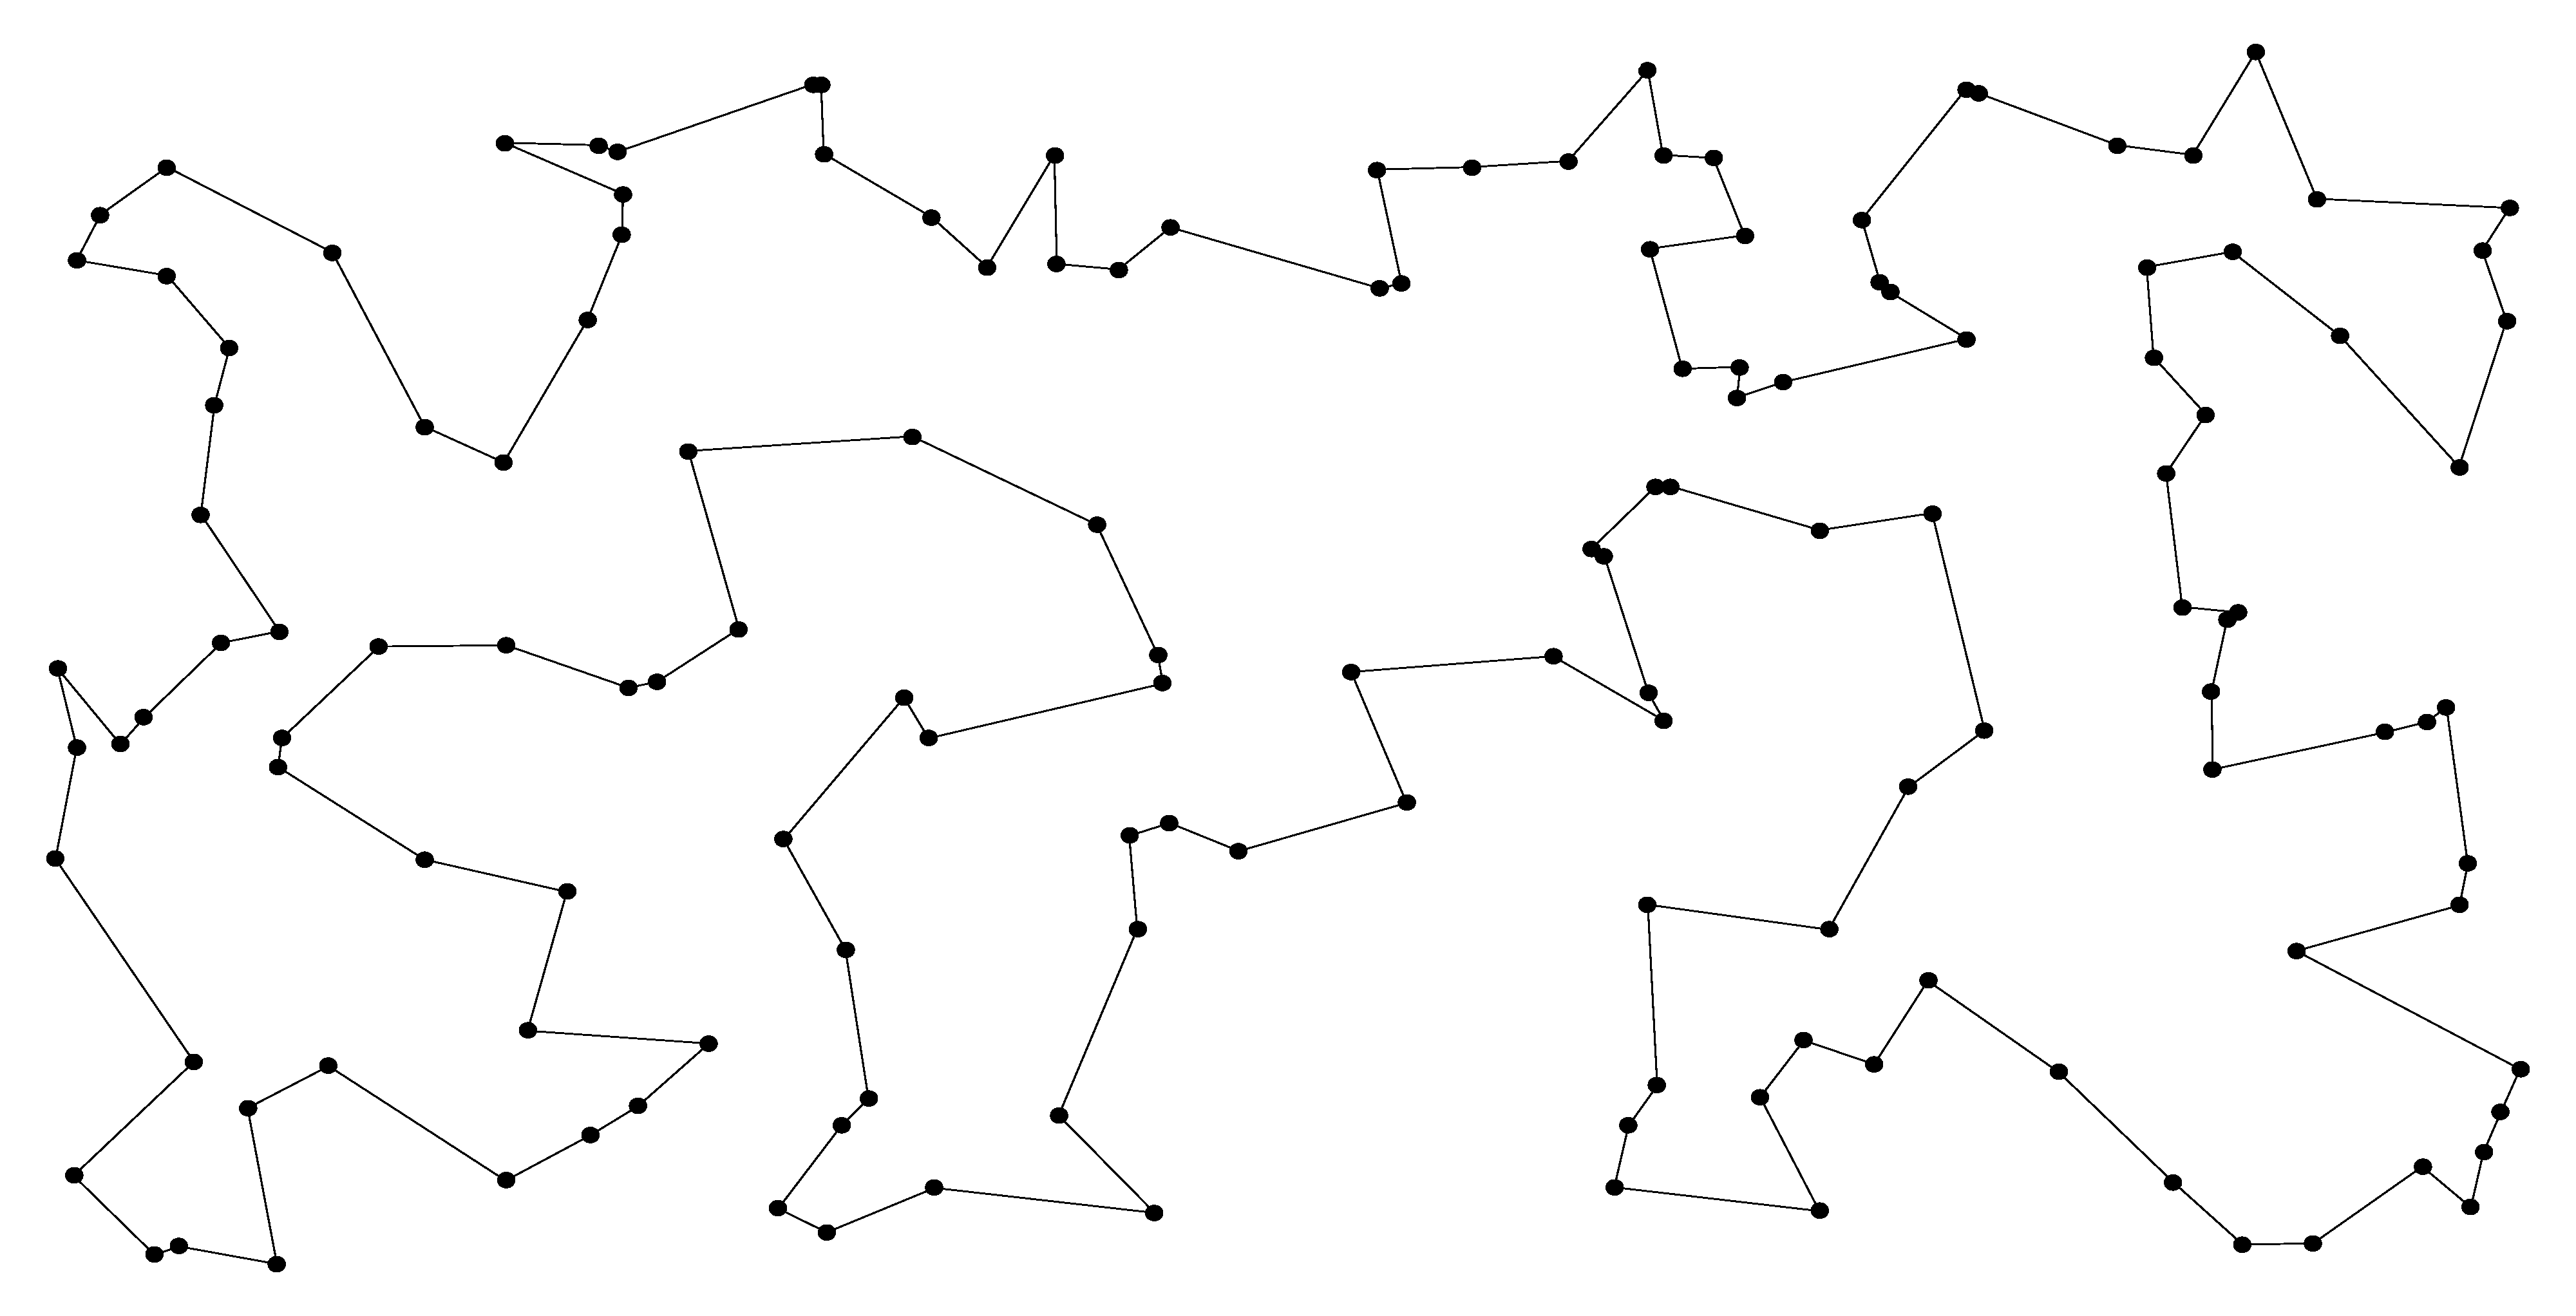
\includegraphics[scale=0.15]{tsp_example}
	\caption{A solution of instance kroA150}
\end{figure}
Therefore, the function to minimize is:
\[
    cost(\pi) = \sum_{i=1}^{n-1} c(v_i, v_{i+1}) + c(v_n,v_1)
\]
where $\pi = (v_1,v_2,\ldots,v_n)$ represents the order in which the nodes (cities) are visited, and $c(v_i,v_j)$ 
represents the cost of traveling from node $v_i$ to node $v_j$.
\section{Complexity of TSP}

The Traveling Salesman Problem (TSP) is renowned not only for its practical applications but also for its classification as an NP-hard problem, signifying its computational complexity and the absence of an efficient algorithm that guarantees an optimal solution within a reasonable timeframe.\newline
This classification as an NP-hard problem implies that as the number of cities to be visited increases, the computation required to find the optimal route escalates exponentially. The TSP's intricate nature lies in its combinatorial explosion: with n cities, the number of possible routes to consider is $(n-1)!/2$, making exhaustive exploration unfeasible for large instances. This exponential growth propels the problem into the realm of computational intractability, where conventional computing methods struggle to provide optimal solutions in a reasonable time frame.\newline
Efforts to solve the TSP have focused on devising algorithms that offer approximate solutions or heuristics that navigate the expansive solution space more efficiently. While exact algorithms exist, such as branch-and-bound techniques, their scalability diminishes as the problem size increases. Heuristic approaches, on the other hand, aim to find near-optimal solutions within acceptable time frames by sacrificing guaranteed optimality for computational tractability.



\chapter{Coding Approaches}

In this chapter, we will explore some low-level implementation details common to most algorithms discussed in the following chapters, as well as some important tricks and decisions taken to improve the quality and efficiencency of the code during the development of the project.

\section{Approaches to Cost Function}

In the TSP, the factor that determines whether a path in a graph is good or not is its overall cost, which represents the sum of all the edges visited along that path.
In this project, we used instances from TSPLIB\cite{tsplib} in order to provide a wide variety of graphs for experimentation.
This section will explore three different approaches for determining the cost of each edge.

\subsection{TSPLIB Specifications}

We focused exclusively on instances where the cost of the edges in the TSP graph could be computed using specific formulas.
In these instances, each node is assigned fixed coordinates, in our case $x$ and $y$ coordinates.
Using these coordinates, the distance between each pair of nodes can be calculated using the appropriate formula according to TSPLIB specifications.
We limited ourself in the implementation of only the most popular distance functions:
\begin{itemize}
    \item EUC\_2D: $round(\sqrt{(x_1 - x_2)^2 + (x_1 - x_2)^2})$
    \item MAX\_2D: $round(max(|x_1 - x_2|,|x_1 - x_2|))$
    \item MAN\_2D: $round(|x_1 - x_2| + |x_1 - x_2|)$
    \item CEIL\_2D: $ceil(\sqrt{(x_1 - x_2)^2 + (x_1 - x_2)^2})$
    \item ATT: \qquad $round(\sqrt{(x_1 - x_2)^2 + (x_1 - x_2)^2}/10)$
\end{itemize}
Where $round(k)$ returns the integer number closest to $k$ and $ceil(k)$ returns the smallest integers greater or equal than $k$.

\subsection{Basic approach}

The first and simplest method involves computing the cost each time it is needed. 
The main advantages of this approach are its inherent simplicity and its $O(2n)$ memory requirement, as it only needs to store the coordinates of the nodes in memory.
Its greatest drawback is the slow execution speed.

In the TSPLIB specifications the majority of the cost functions, which are the same used during all the testing, include some computationally expensive operations.
The square root operation is one of these, as it usually requires an iterative algorithm, like the Newton's method\cite{newtonMethod}, to be computed.
Nowadays most modern computer architectures include a hardware dedicated instructions, which can be many times faster when compared to the software conterparts, yet they still require several CPU cycles in order to be executed.
In order to take advantage of these specialized instructions some additional parameters are required when compiling the code\footnote{\textit{gcc} requires the parameter "-march=native"}.

A further improvement consists in allowing the compiler to stray from the need of computing exact results and approximate the results\footnote{\textit{gcc} requires the parameter "-ffast-math"}.
This type of optimization greatly increases performance of this approach, as shown by \figurename{ \ref{fig:baseHWSpecific}}, however it can generate inaccurate results.
A possible implementation which allows the use this optimization without sacrificing accuracy would be to implement suitable functions in another source file, which will then be compiled using the compiler's built-in tricks and approximations.

\begin{figure}[htbp]
    \centering
    \begin{tikzpicture}
        \begin{axis}[
            width=11cm, height=8cm,
            ymajorgrids=true,
            grid style={dashed,gray!30},
            xlabel=Instance size,
            ylabel=Speedup,
            ymin=1, ymax=2,
            legend style={at={(0.02,0.98)},anchor=north west,legend columns=-1},
            symbolic x coords={100,500,1000,5000,10000},
            log ticks with fixed point,
            xtick=data,
            ytick={1,1.2,1.4,1.6,1.8,2},
            %yticklabels={0\%,20\%,40\%,60\%,80\%,100\%},
            ybar, 
                    ]
            \addplot[Blue,fill] table[x=n, y=cmpbase_hwinstructions, col sep=semicolon] {csv/cmp_2opt.csv};
        \end{axis}
    \end{tikzpicture}
    \caption{Speedup of the use of the "-ffasth-math" compiler flag with the Base approach in 2Opt.} \label{fig:baseHWSpecific}
\end{figure}

The outputs given by these functions should be checked against accurate data, which can be easily done by recomputing the costs of involved edges using accurate methods.
Of course if this check should be performed every time the cost is computed the speed advantage would be lost, that is why we only check the cost before performing a modification to a solution.

Even with all the optimization described above implemented, this approach remains the slowest one, as we will see in the comparision section.

\subsection{Cost-Matrix approach}

The Cost-Matrix approach consists in storing the cost of the edges of the graph in a matrix $A$ of size $n^2$, where each element $a_{i,j}$ represents the cost of edge $e_{i,j}$.
In this method, the costs are computed just once at the start of the execution.
Once the matrix $A$ is initialized, the cost of any edge in the graph can be accessed by retrieving the corresponding value from $A$.

The main advantage of this approach is the ability to obtain the cost of all edges without the need for recalculating them, avoiding the overhead of live computation.
However, despite this significant benefit, there are some major drawbacks.

The first is memory utilization: it requires $O(n^2 + 2n)$ memory to store both the matrix and the coordinates.
It is worth noting that matrix $A$ is symmetric, and the main diagonal consists entirely of zeros, which means memory usage can be reduced to $O(n^2/2-n+2n)$.
However, this memory optimization results in a more complex method of accessing the matrix, as the direct correspondence between edges and matrix elements would be lost.

\begin{figure}[htbp]
    \centering
    \begin{tikzpicture}
        \begin{axis}[
            width=11cm, height=8cm,
            ymajorgrids=true,
            grid style={dashed,gray!30},
            xlabel=Instance size,
            ylabel=Speedup,
            ymin=1, ymax=6,
            legend style={at={(0.02,0.98)},anchor=north west,legend columns=1},
            symbolic x coords={100,500,1000,5000,10000},
            log ticks with fixed point,
            xtick=data,
            ytick={2,3,4,5},
            %yticklabels={100\%,200\%,300\%,400\%},
            ybar, 
                    ]
            \addplot[Blue,fill] table[x=n, y=cmpmatrix_rowmajor, col sep=semicolon] {csv/cmp_2opt.csv};
        \end{axis}
    \end{tikzpicture}
    \caption{Speedup of row-major indexing against column-major indexing with the Cost-Matrix approach in 2Opt.} \label{fig:matrixBadIndex}
\end{figure}

The second major drawback lies in how modern computers handle memory.
Main memory is often a significant bottleneck for most algorithms, to the extent that the time complexity of algorithms is often measured by estimating the number of memory accesses performed.
To improve performance, caching was introduced in comptuter architectures.
Caching involves storing frequently accessed portions of memory in faster memory pools, improving the overall speed of memory access.
With this in mind, cache efficiency is an important factor to consider when comparing the performance of this approach to others.
The issue arises when an algorithm requires repeated access to locations in $A$ that are neither close together nor consistent, which can significantly reduce performance.
A clear example of this can be observed in the performance difference between using row-major indexing versus column-major indexing in $A$.
This is demonstrated in \figurename{ \ref{fig:matrixBadIndex}}, in which the speed difference increases with the size of $A$, which results in lower cache efficiency in the column-major indexing.

\subsection{AVX approach}
To avoid the drawbacks of the two methodologies presented, we decided to try a different implementation.
AVX (Advanced Vector Extensions)\cite{avxWikipedia} is a set of CPU instructions designed to enhance performance by enabling parallel processing of multiple data points with a single instruction.
This approach utilizes these kind of SIMD (Single Instruction Multiple Data) extensions to achieve benefits like increased speed and lower memory usage, at the cost of simplicity: AVX code is significantly more difficult to write and debug.

In simple terms, this method extends the Basic approach by computing multiple edge costs simultaneously, at roughly the same computational cost as calculating a single one.
More specifically, AVX registers are 256 bits in size and support various operations and data types. 
In this project, we chose to use 32-bit floating-point representation for both node coordinates and edge costs.
This allows a single AVX register to hold a vector of eight values, effectively performing eight computations simultaneously.
If higher precision is required, AVX instructions also support 64-bit double-precision floating-point numbers, but with the limitation of processing only four elements at a time, which is half compared to our implementation.

The simplicity of the code is sacrificed in several ways.
The first challenge is the need to arrange the data in a suitable manner so that the vectors loaded into the AVX registers are consistent and not scattered across memory.
To tackle this we used two extra arrays in which the coordinates of the nodes are kept, sorted according to the order in which a solution visit them.
A second challenge arised from handling conditional statements involving individual variables within the eight-elements packed vectors.
This was a bit trickier since it required to perform the conditional statements to whole vectors using specific instructions, save the result as another \textit{mask} vector and then us that vector to move data accrodingly.
Other technical difficulties involve loading the final elements of an array, which can result in loading unintended variables into the register and potentially invalidating the entire computation if not handled properly.
To fix this we simply allocated a bit more memory for each vector in which we stored the value of infinity, such that any computation involved with infinity would result in a \textit{NaN} or infinity itself.

The use of AVX paves the way for further optimizations based on approximation, this time without solely relying on a compiler flag is in the basic approach.
Specifically, the square root operation is optimized by using instructions that perform the \textit{approximated reciprocal square root} and \textit{approximated reciprocal} functions.
This allows an approximation of the square root function to be obtained in a significantly shorter time frame, thanks to the improved latency and throughput of these instructions.
Of course, this type of computation can only be used when looking for a minimum or a maximum between edges or some function involving them, and the final result should always be verified with the more accurate function.

\begin{figure}[htbp]
    \centering
    \begin{tikzpicture}
        \begin{axis}[
            width=11cm, height=8cm,
            ymajorgrids=true,
            grid style={dashed,gray!30},
            xlabel=Instance size,
            ylabel=Speedup,
            ymin=1, ymax=1.6,
            legend style={at={(0.02,0.98)},anchor=north west,legend columns=-1},
            symbolic x coords={100,500,1000,5000,10000},
            log ticks with fixed point,
            xtick=data,
            ytick={1,1.1,1.2,1.3,1.4,1.5,1.6},
            %yticklabels={0\%,10\%,20\%,30\%,40\%,50\%,60\%},
            ybar, 
                    ]
            \addplot[Blue,fill] table[x=n, y=cmpavx_approx, col sep=semicolon] {csv/cmp_2opt.csv};
        \end{axis}
    \end{tikzpicture}
    \caption{Speedup of approximated edge costs with the AVX approach in 2Opt.} \label{fig:avxApprox}
\end{figure}

\subsection{Performance Comparison}

\begin{figure}[htbp]
    \centering
    \begin{tikzpicture}
        \begin{axis}[
            width=11cm, height=8cm,
            ymajorgrids=true,
            grid style={dashed,gray!30},
            xlabel=Instance size,
            ymin=0, ymax=9,
            ylabel=Speedup,
            legend style={at={(0.02,0.98)},anchor=north west,legend columns=-1},
            symbolic x coords={100,500,1000,5000,10000},
            log ticks with fixed point,
            xtick=data,
            ytick={1,2,3,4,5,6,7,8},
            % yticklabels={100\%,200\%,300\%,400\%,500\%,600\%,700\%,800\%},
            ybar, 
                    ]
            \addplot[Blue,fill] table[x=n, y=ones, col sep=semicolon] {csv/cmp_2opt.csv};
            \addplot[Red,fill] table[x=n, y=cmp_matrix, col sep=semicolon] {csv/cmp_2opt.csv};
            \addplot[Green,fill] table[x=n, y=cmp_avx, col sep=semicolon] {csv/cmp_2opt.csv};
            \legend{Basic,Matrix,AVX}
        \end{axis}
    \end{tikzpicture}
    \caption{Comparison of all three approaches in 2-Opt (measurment were taken using the best optimizations found for each approach).} \label{fig:avxShowcase}
\end{figure}

Comparing these three approaches is complex due to numerous factors.
For example, cache efficiency may be better in some TSP instances than in others, depending on how sequentially the cost matrix is accessed.
To minimize these factors as much as possible, data was gathered using multiple instance sizes, with the most common cost function (EUC\_2D).

\figurename{ \ref{fig:avxShowcase}} compares all three methods, scaled relative to the Basic approach.
As expected, the Cost-Matrix method is faster than the Basic method for smaller instances but loses its advantage as the instance size increases, likely because the Cost-Matrix becomes too large for the CPU cache.
Throughout the testing, the AVX approach consistently proved to be the fastest by a significant margin in every scenario.
However, it should be noted that the AVX method yielded unstable results on smaller instances (fewer than 100 nodes), occasionally performing slower than the Cost-Matrix method.

\section{Multithreading}

\begin{figure}[htbp]
    \centering
    \begin{tikzpicture}
        \begin{axis}[
            % title={Multithreading speedup of 2-Opt parallel implementation},
            xlabel={Number of Threads},
            ylabel={Speedup},
            xmin=1, xmax=8,
            ymin=1, ymax=8,
            xtick={1,2,3,4,5,6,7,8},%,10,12,14,16,18,20},
            ytick={1,2,3,4,5,6,7,8},%,9,10,11,12,13,14,15,16},
            legend style={at={(0.98,0.02)},anchor=south east,legend columns=1},
            ymajorgrids=true,
            xmajorgrids=true,
            grid style=dashed,
        ]
        
        \addplot[Blue,mark=square] table[x=cores, y=nn100, col sep=semicolon] {csv/MT.csv};
        \addplot[Red,mark=o] table[x=cores, y=nn1000, col sep=semicolon] {csv/MT.csv};
        \addplot[Green,mark=triangle] table[x=cores, y=nn10000, col sep=semicolon] {csv/MT.csv};
        \addlegendentry{n=100}
        \addlegendentry{n=1000}
        \addlegendentry{n=10000}
            
        \end{axis}
    \end{tikzpicture}
	\caption{Multithreading speedup of Nearest Neighbor parallel implementation.} \label{fig:multithreadNN}
\end{figure}

\begin{figure}[htbp]
    \centering
    \begin{tikzpicture}
        \begin{axis}[
            % title={Multithreading speedup of 2-Opt parallel implementation},
            xlabel={Number of Threads},
            ylabel={Speedup},
            xmin=1, xmax=8,
            ymin=0, ymax=8,
            xtick={1,2,3,4,5,6,7,8},
            ytick={0,1,2,3,4,5,6,7,8},
            legend style={at={(0.02,0.98)},anchor=north west,legend columns=2},
            ymajorgrids=true,
            xmajorgrids=true,
            grid style=dashed,
        ]
        
        \addplot[SkyBlue,mark=square] table[x=cores, y=2opt100, col sep=semicolon] {csv/MT.csv};
        \addplot[Red,mark=o] table[x=cores, y=2opt500, col sep=semicolon] {csv/MT.csv};
        \addplot[Purple,mark=triangle] table[x=cores, y=2opt1000, col sep=semicolon] {csv/MT.csv};
        \addplot[Blue,mark=diamond] table[x=cores, y=2opt5000, col sep=semicolon] {csv/MT.csv};
        \addplot[Green,mark=star] table[x=cores, y=2opt10000, col sep=semicolon] {csv/MT.csv};
        \addlegendentry{n=100}
        \addlegendentry{n=500}
        \addlegendentry{n=1000}
        \addlegendentry{n=5000}
        \addlegendentry{n=10000}
            
        \end{axis}
    \end{tikzpicture}
	\caption{Multithreading speedup of 2-Opt parallel implementation.} \label{fig:multithread2opt}
\end{figure}

Multithreading is a programming technique that allows a computer program to perform multiple tasks concurrently, by dividing its execution into smaller threads of execution that can run independently.

In most of the algorithms implemented, multithreading consists in running the same code on different threads, each with its own randomization.
This is achieved by assigning each thread a different random state value, allowing it to explore different solutions compared to the other threads.

During the computations, the worker threads share the globally best solution found up to that point.
As a result, at the end of the execution, this solution is provided as the output.
This implementation minimizes interaction between threads, allowing for optimal speedup, as shown in \figurename{ \ref{fig:multithreadNN}}.
The fact that smaller instances seem to perform slightly worse is likely due to the shorter execution time of the algorithm, which results in threads spending more time synchronizing the best solution among themselves.

Although this parallel design is commonly used in our algorithm implementations, it is not always applicable.
For example, algorithms that use CPLEX, which is inherently designed to run on multiple threads, do not rely on this approach.

Another example is the 2-Opt and 3-Opt algorithms.
Since these algorithms do not use randomization, the previous type of parallelization would result in each thread producing the same solution.
In these cases, we implemented a straightforward parallelization of the original serial algorithm to optimize large instances in a reasonable amount of time.
The algorithm's speedup and scalability depend on the instance size, as shown in \figurename{ \ref{fig:multithread2opt}}.

\section{Solution Representation}

Choosing the representation for the TSP solution in memory can be challenging due to the many available options, each with its own pros and cons.
We selected the \textbf{Path of Indices} as the primary representation method.
This approach uses a single array, with a size equal to the number of nodes, where the indices of the nodes are stored in the order of their occurrence in the tour.
This representation offers a main advantage that we relied on: the edges in the tour can be easily determined by examining the connections between nodes in adjacent positions in the solution.
This is advantageous for the 2-Opt and 3-Opt algorithms because this representation implicitly encodes the edges of the tour, allowing the solution to be explored while maintaining high cache efficiency.
However, it should be noted that to fully utilize this advantage, especially when using the AVX approach, the first node must also be appended to the end of the array to represent the last visited edge in the solution.

When not using the Cost-Matrix approach, it is useful to keep a copy of the coordinates $X$ and $Y$ sorted to match the solution order.
This optimization significantly improved the speed of AVX computation, as a fast \textit{load} instruction could be used instead of a \textit{gather} instruction, which involves multiple steps to be executed.
A small improvement was also observed on the Basic approach, likely due to increased memory access locality, which reduced the overall number of cache misses.

\subsection{Cost-Cache}

Throughout our implementations, you may encounter an array named \textbf{Cost-Cache}.
As its name suggests, this array contains the cost of each edge in the solution, sorted according to the order in which the edges are visited.
It allows to gain performance even when using the Cost-Matrix approach, even if it is only a small improvement.

Initially conceived as a simple caching method to improve the speed of some algorithms, it now plays a crucial role in our implementation of the Tabu Search algorithm.

\begin{figure}[htbp]
    \centering
    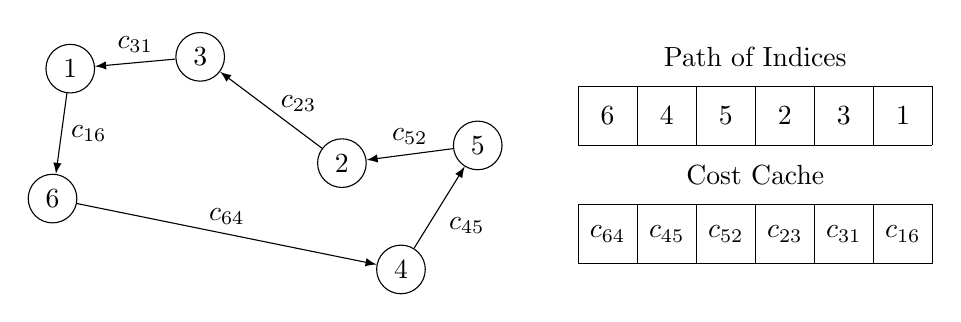
\begin{tikzpicture}[scale=0.75]
        \node[circle, draw, fill=white] (A) at (2.6, 4) {3};
        \node[circle, draw, fill=white] (B) at (0.4, 3.8) {1};
        \node[circle, draw, fill=white] (C) at (0.1, 1.6) {6};
        \node[circle, draw, fill=white] (D) at (6, 0.4) {4};
        \node[circle, draw, fill=white] (E) at (7.3, 2.5) {5};
        \node[circle, draw, fill=white] (F) at (5, 2.2) {2};
    
       \draw[-latex] (A) to node[above,] {$c_{31}$} (B);
		\draw[-latex] (B) to node[right] {$c_{16}$} (C);
		\draw[-latex] (C) to node[above] {$c_{64}$} (D);
		\draw[-latex] (D) to node[below right] {$c_{45}$} (E);
		\draw[-latex] (E) to node[above] {$c_{52}$} (F);
		\draw[-latex] (F) to node[above right, yshift=-4] {$c_{23}$} (A);
	
		\begin{scope}[shift={(9, 1.5)}]
			\draw (0,1) grid (6,2);
			\path (.5,.5) (0.5,1.5) node{$6$} ++(1,0) node{$4$} ++(1,0) node{$5$} ++(1,0) node{$2$} ++(1,0) node{$3$} ++(1,0) node{$1$};
			\draw (3,2.5) node{Path of Indices};
        \end{scope} 

		\begin{scope}[shift={(9, -0.5)}]
			\draw (0,1) grid (6,2);
			\path (.5,.5) (0.5,1.5) node{$c_{64}$} ++(1,0) node{$c_{45}$} ++(1,0) node{$c_{52}$} ++(1,0) node{$c_{23}$} ++(1,0) node{$c_{31}$} ++(1,0) node{$c_{16}$};
			\draw (3,2.5) node{Cost Cache};
        \end{scope}    

    \end{tikzpicture}
    \caption{Representation of the Cost-Cache.}
    \label{fig:solRepresentationExample}
\end{figure}

\begin{figure}[htbp]
    \centering
    \begin{tikzpicture}
        \begin{axis}[
            width=11cm, height=8cm,
            ymajorgrids=true,
            grid style={dashed,gray!30},
            xlabel=Instance size,
            ylabel=Speedup,
            ymin=1, ymax=1.5,
            legend style={at={(0.02,0.98)},anchor=north west,legend columns=-1},
            symbolic x coords={100,500,1000,5000,10000},
            log ticks with fixed point,
            xtick=data,
            ytick={1,1.1,1.2,1.3,1.4},
            yticklabels={0\%,10\%,20\%,30\%,40\%},
            ybar, 
                    ]
            \addplot[Blue,fill] table[x=n, y=cmpcc_base, col sep=semicolon] {csv/cmp_2opt.csv};
            \addplot[Red,fill] table[x=n, y=cmpcc_matrix, col sep=semicolon] {csv/cmp_2opt.csv};
            \addplot[Green,fill] table[x=n, y=cmpcc_avx_approx, col sep=semicolon] {csv/cmp_2opt.csv};
            \legend{Basic,Matrix,AVX}
        \end{axis}
    \end{tikzpicture}
    \caption{Speedup gained by each approach using the cost cache in 2-Opt.} \label{fig:costCacheShowcase} 
\end{figure}

\subsection{Solution Cost Precision}

Throughout the execution of any implemented algorithm, the overall cost of the solution being generated or optimized constantly changes.
During the project's development, we found it useful to update this value with each modification made to a solution.
Although this is a good practice for debugging the algorithms, it can sometimes lead to precision issues.
These issues stem from the limitations of floating-point standard representation.
For example, consider two numbers, $a=10^8$ and $b=1.53$.
When using the 32-bit floating-point standard, $a+b=10^8=a$, because the bits of the mantissa of $b$ are \textit{out of bounds} compared to those of $a$.
This situation can arise when a solution has been optimized, and its overall cost is the result of adding or subtracting minor improvements throughout the optimization process.
As a result, when the cost of the solution is recomputed at the end of the optimization procedure - usually to verify if it matches the current solution cost - these values might differ slightly. 
This is especially true for very large instances.

A solution to this problem is to store the cost of the solution in a higher precision variable.
Extending the variable to 64 bits resolved the issue for the most part, but did not completely eliminate it.

The best solution we found was to switch from floating-point to fixed-point representation.
Since fixed-point representation does not have a standard implementation in the C language, we implemented one ourselves.
We used 128 bits, with 64 for the integer part and the remaining 64 for the fractional part.
This effectively eliminated all the precision issues we encountered, although it's not without drawbacks: fixed-point variables are less flexible with large ranges compared to floating-point ones.

This precision problem is only a concern during debugging, as in production, it may be sufficient to simply recompute the cost of the solution when necessary.


\chapter{Heuristics}

\section{Nearest Neighbor}

Nearest Neighbor (NN) is a simple, intuive and yet relatively effective greedy algorithm designed to find a feasible solution to the Traveling Salesman Problem.
As its name suggests, NN consists of building a solution to a TSP instance by selecting the nearest node to the last visited one.
The key steps of the algorithm are:
\begin{enumerate}
    \item choose an initial node as the starting location.
    \item from the current point, identify the nearest unvisited point.
    \item move to the selected node and mark it as visited.
    \item repeat from step 2 until all the nodes are marked as visited.
\end{enumerate}

\begin{algorithm}[htbp]
	\TitleOfAlgo{\textbf{Nearest Neighbor}}
    \SetKwInOut{Input}{Input}
    \SetKwInOut{Output}{Output}
    \Input{
        Graph $G(V,E)$ fully connected \newline
        $c_{ij}=$ cost of $edge(i,j) \in |E|$ \newline
        Starting vertex $s$
    }
    \Output{A tour $T$ of $G$ and its cost $b$}
    \BlankLine
    $T \gets \{s\}$\\
    $v \gets s$\\
    $b \gets 0$\\
    \While{$|T| < |V|$}{
        identify $u \in V/T$ s.t. $c_{vu} \leq c_{vj}$, $\forall$ $j \in V/(T \cup {u})$\\
        $T \gets T \cup \{u\}$\\
        $b \gets b + c_{vu}$\\
        $v \gets u$\\
    }
    $b \gets b + c_{vs}$\\
    \Return $tour$, $b$\\
\end{algorithm}

NN returns a feasible solution regardless of its starting position; however, the resulting solution usually depends on the starting point.
Therefore, it's good practice to set a time limit and restart the algorithm each time with a different starting point, while keeping track of the best solution found so far.
While NN is a good starting option, further refinement using a metaheuristic is usually necessary, as the initial solution is often far from optimal.

\subsection{GRASP}
The above implementation limits itself in producing solutions only depending on the starting node.
This means that after starting NN on all the nodes of the instance no more new solution will be found.
The \textbf{greedy randomized adaptive search procedure} (also known as \textbf{GRASP}) is a technique that allows to introduce a degree of randomization into greedy algorithms like this one.
We implemented the GRASP technique in our algorithm with two different settings:
\begin{enumerate}
    \item \textit{almostbest}: 
    while searching for the nearest node, the algorithm keeps track of the $k$ nearest nodes, and then one of the nodes from this list is selected according to a probability rule.
    A simple selection method consists in sorting the list elements from nearest to farthest, and then, starting with the first element, rejecting it based on a probability $p$.
    If an element in the list is rejected, the next element is considered as a candidate, and the rejection process continues until either an element is accepted or the end of the list is reached, in which case the last element is chosen.
    \item \textit{random}:
    in this implementation we simply add a completely random node as successor in the solution.
    The probability at which a random successor is chosen over the optimal one is set during the initilization phase.
\end{enumerate}
Both these enhancements allow NN to run indefinitevly while still finding different solutions.
In this setting, the use of a time limit is necessary.

% \subsection{Implementation}
%% ????
% We have some options on how we want to run NN. First off we can decide whether to use GRASP or not, but we can also configure 
% how many threads we want to use, if we want to compute the distances between points every time needed or use a matrix to store 
% them, or use AVX functions when possible to improve the performances. We can also choose to use 2-opt or 3-opt after finding a 
% solution to improve its cost, or we can just leave it as is.

% ######## Already in coding approaches
% By using the cost matrix to store the weight of all the edges we can speed up the computation, but this will require a tradeoff 
% in memory, O(n²) more specifically, where n is the number of nodes in the instance. Considering that we are storing nodes in a 
% matrix of float variables, this is still good for many applications, e.g. an instance of 10000 nodes will require 0.37 GB of 
% memory. This changes when we take into consideration larger instances, like the largest one in TSPlib, which includes 85900 
% nodes and would require just short of 27.5 GB of memory.
% This is why we implemented the computation of the edge weight on the fly both normally and with AVX instructions, which allows 
% us to find the solution of more complex instances.

% ????
% The function that handles the application of the heuristic is NearestNeighbor, to which we pass both the instance of the 
% problem and the time limit. The application of GRASP and the creation of the required number of threads is handled here.
% We launch each thread with the function loopNearestNeighbor, which loops the application of applyNearestNeighbor selecting 
% a different starting node every time until all nodes have been used or the time limit is reached.
% At all time we keep track of the best solution found so far, which is then the one returned by NearestNeighbor. When the 
% solution is return 2-opt and 3-opt will be applied as desired.

% This heuristic presents two main problems: the first is that, been a greedy algorithm, at each iteration we always visit 
% the next closest point and this leads to the creation of many intersection between the edges of the solution, which are 
% clearly inefficient (we deal with this problem using 2-opt or 3-opt). The second one is that is a deterministic algorithm, 
% which means that if we run it from the same starting node multiple times the solution will never change, so the number 
% of total solutions obtainable is limited to the number of nodes.

\subsection{Performance}

Before checking how NN performs against the optimal solution it is interesting to check if some values of probability for GRASP yield a higher quality solution and if a GRASP setting works better than the other.

\subsubsection{GRASP \textit{almostbest}}

\begin{figure}[htbp]
	\centering
	\begin{tikzpicture}
        \begin{axis}[
            xlabel={Cost Ratio},
            xmin=1, xmax=1.1,
            ymin=0, ymax=82,
            xtick={},
            ytick=\empty,
            legend style={at={(0.98,0.02)},anchor=south east,legend columns=1},
			legend cell align={left},
            xmajorgrids=true,
            grid style=dashed,
        ]
        
        \addplot[Blue,mark=square,mark size=1.5] table[x=cmp0_0.1,y=idx, col sep=semicolon] {csv/nn_almostbest.csv}; 
        \addplot[Red,mark=o,mark size=1.5] table[x=cmp0_0.05,y=idx, col sep=semicolon] {csv/nn_almostbest.csv};
        \addplot[Green,mark=triangle,mark size=1.5] table[x=cmp0_0.01,y=idx, col sep=semicolon] {csv/nn_almostbest.csv}; 
        \addlegendentry{0.1} 
        \addlegendentry{0.05}
        \addlegendentry{0.01}
            
        \end{axis}
    \end{tikzpicture}
	\caption{Comparison between different probabilities in NN with GRASP set to \textit{almostbest}}
    \label{fig:nnAlmostbestCmp0}
\end{figure}

From \figurename{ \ref{fig:nnAlmostbestCmp0}} it's clear that the best probability value is $0.05$.
However, by gathering more data and studying the relation between the best GRASP value for each instance and the size of the instance, we found that this conclusion is not exactly accurate.
There might be various reasons to explain these results, but lacking both the tools and the time, we did not investigate further.

\begin{figure}[htbp]
	\centering
	\begin{tikzpicture}
        \begin{axis}[
            ylabel={Probability value},
            xlabel={Number of Nodes},
            domain=48:85901,
            ymin=0, ymax=0.15,
            xmin=48, xmax=85900,
            xtick={},
            ytick={0.12, 0.1, 0.085, 0.075, 0.065, 0.05, 0.03, 0.01, 0},
            yticklabel style={/pgf/number format/fixed, /pgf/number format/precision=3},
            xmode=log,
            legend style={at={(0.98,0.98)},anchor=north east,legend columns=1},
			legend cell align={left},
            ymajorgrids=true,
            xmajorgrids=true,
            grid style=dashed,
        ]
        
        \addplot[Red,mark=*,mark size=1, only marks] table[y=bestParam, x=n, col sep=semicolon] {csv/nn_almostbest.csv};
        \addplot[Blue,thick] plot (\x,{exp(0.68515)*\x^(-0.6464)});
        \addlegendentry{Best records} 
        \addlegendentry{Learned function}
            
        \end{axis}
    \end{tikzpicture}
	\caption{Best probability value for NN GRASP set to \textit{almostbest} w.r.t. the size of the instance}
    \label{fig:nnAlmostbestFunction}
\end{figure}

\begin{figure}[htbp]
	\centering
	\begin{tikzpicture}
        \begin{axis}[
            xlabel={Cost Ratio},
            xmin=1, xmax=1.05,
            ymin=0, ymax=82,
            xtick={},
            ytick=\empty,
            legend style={at={(0.98,0.02)},anchor=south east,legend columns=1},
			legend cell align={left},
            xmajorgrids=true,
            grid style=dashed,
        ]
        
        \addplot[Blue,mark=square,mark size=1.5] table[x=cmp1_0.1,y=idx, col sep=semicolon] {csv/nn_almostbest.csv}; 
        \addplot[Red,mark=o,mark size=1.5] table[x=cmp1_0.05,y=idx, col sep=semicolon] {csv/nn_almostbest.csv};
        \addplot[Green,mark=triangle,mark size=1.5] table[x=cmp1_0.01,y=idx, col sep=semicolon] {csv/nn_almostbest.csv}; 
        \addplot[Purple,mark=star,mark size=1.5] table[x=cmp1_best,y=idx, col sep=semicolon] {csv/nn_almostbest.csv}; 
        \addlegendentry{0.1} 
        \addlegendentry{0.05}
        \addlegendentry{0.01}
        \addlegendentry{dynamic}
            
        \end{axis}
    \end{tikzpicture}
	\caption{Comparison between different probabilities, including dynamic probability mode, in NN with GRASP set to \textit{almostbest}}
    \label{fig:nnAlmostbestCmp1}
\end{figure}

However, since we noticed this behavior, with the use of machine learning tools, we found an exponential curve to approximate the best probability value of GRASP \textit{almostbest}, as shown in \figurename{ \ref{fig:nnAlmostbestFunction}}.
We called this method of selecting the GRASP probability as \textbf{dynamic probability mode}.
We then proceeded to gather more data using the dynamic probability mode.
The results, shown in \figurename{ \ref{fig:nnAlmostbestCmp1}}, present a slight advantage of the dynamic probability mode over the $0.5$ fixed probability, which was the best value in previous testing.

\subsubsection{GRASP \textit{random}}

Following the same procedure as above we discovered a similar situation.
\figurename{ \ref{fig:nnRandomFunction}} shows the best probability value of GRASP in \textit{random} mode.

\begin{figure}[htbp]
	\centering
	\begin{tikzpicture}
        \begin{axis}[
            ylabel={Probability value},
            xlabel={Number of Nodes},
            domain=48:85901,
            ymin=0, ymax=0.06,
            xmin=48, xmax=85900,
            xtick={},
            ytick={0.05,0.03,0.02,0.01,0.005,0.001},
            xmode=log,
            legend style={at={(0.98,0.98)},anchor=north east,legend columns=1},
			legend cell align={left},
            ymajorgrids=true,
            xmajorgrids=true,
            grid style=dashed,
        ]
        
        \addplot[Red,mark=*,mark size=1, only marks] table[y=bestParam, x=n, col sep=semicolon] {csv/nn_random.csv};
        \addplot[Blue,thick] plot (\x,{\x^(-0.87173)});
        \addlegendentry{Best records} 
        \addlegendentry{Learned function}
            
        \end{axis}
    \end{tikzpicture}
	\caption{Best probability value for NN GRASP set to \textit{random} w.r.t. the size of the instance}
    \label{fig:nnRandomFunction}
\end{figure}

Again, with the use of machine learning algorithms we extracted another exponential function from the best records.
By gathering the necessary data using the dynamic probability mode, we obtained the comparison in \figurename{ \ref{fig:nnRandomCmp1}}, which shows better performance towards the dynamic mode.

\begin{figure}[htbp]
	\centering
	\begin{tikzpicture}
        \begin{axis}[
            xlabel={Cost Ratio},
            xmin=1, xmax=1.2,
            ymin=0, ymax=82,
            xtick={},
            ytick=\empty,
            legend style={at={(0.98,0.02)},anchor=south east,legend columns=1},
			legend cell align={left},
            xmajorgrids=true,
            grid style=dashed,
        ]
        
        \addplot[Blue,mark=square,mark size=1.5] table[x=cmp_0.05,y=idx, col sep=semicolon] {csv/nn_random.csv}; 
        \addplot[Red,mark=o,mark size=1.5] table[x=cmp_0.01,y=idx, col sep=semicolon] {csv/nn_random.csv};
        \addplot[Green,mark=triangle,mark size=1.5] table[x=cmp_0.001,y=idx, col sep=semicolon] {csv/nn_random.csv}; 
        \addplot[Purple,mark=star,mark size=1.5] table[x=cmp_best,y=idx, col sep=semicolon] {csv/nn_random.csv}; 
        \addlegendentry{0.1} 
        \addlegendentry{0.05}
        \addlegendentry{0.01}
        \addlegendentry{dynamic}
            
        \end{axis}
    \end{tikzpicture}
	\caption{Comparison between different probabilities, including dynamic probability mode, in NN with GRASP set to \textit{random}}
    \label{fig:nnRandomCmp1}
\end{figure}

\subsubsection{NN GRASP settings comparison}

Now that the best performing parameters for each mode have been esablished, it is possible to compare all the different implementations of NN between each other.

\begin{figure}[htbp]
	\centering
	\begin{tikzpicture}
        \begin{axis}[
            xlabel={Cost Ratio},
            xmin=1, xmax=1.12,
            ymin=0, ymax=82,
            xtick={},
            ytick=\empty,
            legend style={at={(0.98,0.02)},anchor=south east,legend columns=1},
			legend cell align={left},
            xmajorgrids=true,
            grid style=dashed,
        ]

        \addplot[Blue,mark=square,mark size=1.5] table[x=nn_cmp_nograsp,y=idxExtended, col sep=semicolon] {csv/cmp_nn_em.csv};
        \addplot[Red,mark=o,mark size=1.5] table[x=nn_cmp_almostbest,y=idxExtended, col sep=semicolon] {csv/cmp_nn_em.csv};
        \addplot[Green,mark=triangle,mark size=1.5] table[x=nn_cmp_random,y=idxExtended, col sep=semicolon] {csv/cmp_nn_em.csv};
        \addlegendentry{GRASP Disabled}
        \addlegendentry{GRASP \textit{almostbest}}
        \addlegendentry{GRASP \textit{random}}
            
        \end{axis}
    \end{tikzpicture}
	\caption{Comparison between NN GRASP modes}
    \label{fig:nnCmp}
\end{figure}

% \figurename{ \ref{fig:nnCmp}} clearly shows the GRASP implementations outperforming the canonical implementation of NN by a significant amount.
% While I DON'T KNOW IF I SHOULD WRITE MORE OBVIOUS STUFF ABOUT THIS.

\newpage

\section{Extra Mileage}

The Extra Mileage (EM) heuristic is another greedy algorithm able to find solutions to the TSP, with no guarantees on optimality.
While similar to NN, it comes with a slight variation in the selection process. 
In EM the idea is to minimize the additional \textit{mileage} (or cost) traveled at each iteration, rather than always selecting the nearest unvisited node.
The procedure starts by creating an arbitrary cycle inside the input instance.
A cycle with just two nodes is sufficient to initiate the method.
At each iteration, we consider adding every unvisited node at every possible position of the current cycle, and compute the increase in cost, or the \textit{extra mileage}.
The algorithm continues to add nodes to the solution until there are no nodes left to add.

\begin{algorithm}[H]
	\TitleOfAlgo{\textbf{Extra Mileage}}
    \SetKwInOut{Input}{Input}
    \SetKwInOut{Output}{Output}
    \Input{
        Graph $G(V,E)$ fully connected \newline
        $c_{ij}=$ cost of $edge(i,j) \in |E|$ \newline
        Starting subtour $S$
    }
    \Output{A tour $T$ of $G$ and its cost $b$}
    \BlankLine
    $T \gets S$\\
    $b \gets$ $cost(S)$\\
    \While{{$|T| < |V|$}}{
        identify $w \in V/T$ s.t. $c_{uw} + c_{wv} - c_{uv}$ is minumum $\forall$ $u,v \in T$, $u \neq v$\\
        insert $w$ between $u$, $v$ in $T$\\
        $b \gets b + c_{uw} + c_{wv} - c_{uv}$\\
    }
    \Return $tour$, $b$\\
    
\end{algorithm}

As it was the case with NN, in EM the final solution on a single instance depends on the initialization of the algorithm.
Since we chose to use a cycle composed of only two nodes as initialization of the algorithm, the number of possible initialization is finite.
Therefore, after all the possible initialization have been used, no new solution will appear.
As before, GRASP can be implemented in EM the same exact way we implemented it in NN, with both the settings \textit{almostbest} and \textit{random}.

% \subsection{Implementation}
% Extra mileage, like nearest neighbor, is a "solution builder", it generates a feasible solution starting from just the 
% instance of the problem. Hence, we structured the implementation of this heuristic in a similar concept, maintaining the 
% same configuration options, which are the application of GRASP, the number of threads to use, the computation of the edges' 
% weights on the fly or store them in a matrix, and the application of 2-opt or 3-opt.

% A similar structure is also implemented for the way we apply extra mileage to the instance. The main function that handles 
% all the processes is ExtraMileage, which receives the instance and the time limit, sets GRASP if needed and creates the 
% required number of threads.
% The threads will run the function runExtraMileage until the time limit, launching in loop the function applyExtraMileage, 
% which is the actual function that computes the heuristic.

\subsection{Performance}

\textbf{GRASP \textit{almostbest}}

Suspecting the same behavior observed while gathering data for NN we directly proceded to the study of the best records in the probaility value of GRASP.
In this case there doesn't seem to be any correlation between the probability value and the number of nodes inside an instance, as shown by \figurename{ \ref{fig:emAlmostbestFunction}}.
Since there doesn't seem to be any correlation between the best records and the size of the instances we limited ourselves to simply compare probability values between each other.

\begin{figure}[htbp]
	\centering
	\begin{tikzpicture}
        \begin{axis}[
            ylabel={Probability value},
            xlabel={Number of Nodes},
            ymin=0, ymax=0.6,
            xmin=48, xmax=2393,
            xtick={},
            ytick={0.5,0.4,0.3,0.2,0.15,0.1,0.05,0},
            yticklabel style={/pgf/number format/fixed, /pgf/number format/precision=4},
            xmode=log,
            legend style={at={(0.98,0.98)},anchor=north east,legend columns=1},
			legend cell align={left},
            ymajorgrids=true,
            xmajorgrids=true,
            grid style=dashed,
        ]
        
        \addplot[Red,mark=*,mark size=1, only marks] table[y=bestParam, x=n, col sep=semicolon] {csv/em_almostbest.csv};
        % \addlegendentry{Best records}
            
        \end{axis}
    \end{tikzpicture}
	\caption{Best probability value for EM GRASP set to \textit{almostbest} w.r.t. the size of the instance}
    \label{fig:emAlmostbestFunction}
\end{figure}

\begin{figure}[htbp]
	\centering
	\begin{tikzpicture}
        \begin{axis}[
            xlabel={Cost Ratio},
            xmin=1, xmax=1.04,
            ymin=0, ymax=69,
            xtick={},
            ytick=\empty,
            legend style={at={(0.98,0.02)},anchor=south east,legend columns=1},
			legend cell align={left},
            xmajorgrids=true,
            grid style=dashed,
        ]
        
        \addplot[Blue,mark=square,mark size=1.5] table[x=cmp_0.5,y=idx, col sep=semicolon] {csv/em_almostbest.csv}; 
        \addplot[Red,mark=o,mark size=1.5] table[x=cmp_0.3,y=idx, col sep=semicolon] {csv/em_almostbest.csv};
        \addplot[Green,mark=triangle,mark size=1.5] table[x=cmp_0.1,y=idx, col sep=semicolon] {csv/em_almostbest.csv}; 
        \addplot[Purple,mark=star,mark size=1.5] table[x=cmp_0.01,y=idx, col sep=semicolon] {csv/em_almostbest.csv}; 
        \addlegendentry{0.5} 
        \addlegendentry{0.3}
        \addlegendentry{0.1}
        \addlegendentry{0.01}
            
        \end{axis}
    \end{tikzpicture}
	\caption{Comparison of various values of chance with EM GRASP type \textit{almostbest}}
    \label{fig:emAlmostbestCmp1}
\end{figure}

\textbf{GRASP \textit{random}}

In the case of the GRASP \textit{random} setting, the linear correlation between probability value and instance size appeared once again.
Then we completed the testing the exact same way as before and found the exponential function that outputs the "optimal" probability value based on the instance size.
The results are shown in \figurename{ \ref{fig:emRandomCmp1}} where it's clear that the dynamic probability mode outperformns the fixed one.

\begin{figure}[htbp]
	\centering
	\begin{tikzpicture}
        \begin{axis}[
            ylabel={Probability value},
            xlabel={Number of Nodes},
            domain=48:2393,
            ymin=0, ymax=0.11,
            xmin=48, xmax=2393,
            xtick={},
            ytick={0.1,0.05,0.03,0.02,0.01,0.001},
            yticklabel style={/pgf/number format/fixed, /pgf/number format/precision=3},
            xmode=log,
            legend style={at={(0.98,0.98)},anchor=north east,legend columns=1},
			legend cell align={left},
            ymajorgrids=true,
            xmajorgrids=true,
            grid style=dashed,
        ]
        
        \addplot[Red,mark=*,mark size=1, only marks] table[y=bestParam, x=n, col sep=semicolon] {csv/em_random.csv};
        \addplot[Blue,thick] plot (\x,{\x^(-0.97415)});
        \addlegendentry{Best records}
        \addlegendentry{Learned function}
            
        \end{axis}
    \end{tikzpicture}
	\caption{Best chance for EM GRASP type \textit{random} w.r.t. the size of the instance}
    \label{fig:emRandomFunction}
\end{figure}

\begin{figure}[htbp]
	\centering
	\begin{tikzpicture}
        \begin{axis}[
            xlabel={Cost Ratio},
            xmin=1, xmax=1.04,
            ymin=0, ymax=69,
            xtick={},
            ytick=\empty,
            legend style={at={(0.98,0.02)},anchor=south east,legend columns=1},
			legend cell align={left},
            xmajorgrids=true,
            grid style=dashed,
        ]
        
        \addplot[Blue,mark=square,mark size=1.5] table[x=cmp_0.03,y=idx, col sep=semicolon] {csv/em_random.csv}; 
        \addplot[Red,mark=o,mark size=1.5] table[x=cmp_0.01,y=idx, col sep=semicolon] {csv/em_random.csv};
        \addplot[Green,mark=triangle,mark size=1.5] table[x=cmp_0.001,y=idx, col sep=semicolon] {csv/em_random.csv}; 
        \addplot[Purple,mark=star,mark size=1.5] table[x=cmp_best,y=idx, col sep=semicolon] {csv/em_random.csv}; 
        \addlegendentry{0.03} 
        \addlegendentry{0.01}
        \addlegendentry{0.001}
        \addlegendentry{dynamic}
            
        \end{axis}
    \end{tikzpicture}
	\caption{Comparison between different probabilities, including dynamic probability mode, in EM with GRASP set to \textit{random}}
    \label{fig:emRandomCmp1}
\end{figure}

\subsubsection{EM GRASP settings comparison}

Even though in the \textit{almostbest} setting we weren't able to find any optimal probability/instance-size curve, the \textit{random} is still outperformed by it.
The deterministic execution is the one with the weakest performance, as it was the case for NN, enhancing the ability of GRASP to produce better results simply by using randomization.

\begin{figure}[htbp]
	\centering
	\begin{tikzpicture}
        \begin{axis}[
            xlabel={Cost Ratio},
            xmin=1, xmax=1.07,
            ymin=0, ymax=69,
            xtick={},
            ytick=\empty,
            legend style={at={(0.98,0.02)},anchor=south east,legend columns=1},
			legend cell align={left},
            xmajorgrids=true,
            grid style=dashed,
        ]
        
        \addplot[Blue,mark=square,mark size=1.5] table[x=em_cmp_nograsp,y=idx, col sep=semicolon] {csv/cmp_nn_em.csv};
        \addplot[Red,mark=o,mark size=1.5] table[x=em_cmp_almostbest,y=idx, col sep=semicolon] {csv/cmp_nn_em.csv};
        \addplot[Green,mark=triangle,mark size=1.5] table[x=em_cmp_random,y=idx, col sep=semicolon] {csv/cmp_nn_em.csv};
        \addlegendentry{GRASP Disabled}
        \addlegendentry{GRASP \textit{almostbest}}
        \addlegendentry{GRASP \textit{random}}
            
        \end{axis}
    \end{tikzpicture}
	\caption{Comparison between EM GRASP settings}
    \label{fig:emCmp}
\end{figure}

\section{Comparison}

In this section both NN and EM are compared when executed within the same time limit.
Each heuristic used its most performing settings in this comparison, namely dynamic probability mode with GRASP set to \textit{almostbest}.
It's clear that EM outputs better solutions overall compared to NN.
This is not always the case and the reason of why that happens can be explained by discussing computational complexity.
The NN algorithm has a time complexity of $O(n^2)$ while EM is more expensive, with a complexity of $O(n^3)$.
Then, when the size of the instance becomes very high, the EM heuristic falls behind NN in terms of iterations done each second.
Therefore we can conclude that the cases in which EM perfomed worse than NN are due to the fact that EM did not have enough time to compute enough solutions and find a good one.
These computational complexity considerations are made upon our implementations of the algorithms, since there may be a way to optimize the EM heuristic more.

\begin{figure}[htbp]
	\centering
	\begin{tikzpicture}
        \begin{axis}[
            xlabel={Cost Ratio},
            xmin=1, xmax=1.1,
            ymin=0, ymax=69,
            xtick={},
            ytick=\empty,
            legend style={at={(0.98,0.02)},anchor=south east,legend columns=1},
			legend cell align={left},
            xmajorgrids=true,
            grid style=dashed,
        ]
        
        \addplot[Blue,mark=square,mark size=1.5] table[x=cmp_nn,y=idx, col sep=semicolon] {csv/cmp_nn_em.csv};
        \addplot[Red,mark=o,mark size=1.5] table[x=cmp_em,y=idx, col sep=semicolon] {csv/cmp_nn_em.csv};
        \addlegendentry{NN}
        \addlegendentry{EM}
            
        \end{axis}
    \end{tikzpicture}
	\caption{Comparison the quality of the output of NN and EM}
    \label{fig:cmpNNEMcost}
\end{figure}

\begin{figure}[htbp]
	\centering
	\begin{tikzpicture}
        \begin{loglogaxis}[
            xlabel={Number of nodes},
            ylabel={Iterations/s Ratio},
            xmin=48, xmax=2392,
            ymin=1, ymax=2650,
            xtick={},
            ytick={},
            legend style={at={(0.02,0.98)},anchor=north west,legend columns=1},
			legend cell align={left},
            xmajorgrids=true,
            grid style=dashed,
        ]
        
        \addplot[Blue,mark=square,mark size=1.5] table[y=cmp_iters_nn, x=n, col sep=semicolon] {csv/cmp_nn_em.csv};
        \addplot[Red,mark=o,mark size=1.5] table[y=cmp_iters_em, x=n, col sep=semicolon] {csv/cmp_nn_em.csv};
        \addlegendentry{NN}
        \addlegendentry{EM}
            
        \end{loglogaxis}
    \end{tikzpicture}
	\caption{Comparison the number of iterations NN and EM were able to do within the same time limit.}
    \label{fig:cmpNNEMiter}
\end{figure}


\chapter{Metaheuristics}

\section{What is a metaheuristic?}

A metaheuristic is a problem-solving strategy that consists in a set of steps with the purpose of finding good solutions to optimization problems.
Unlike heuristics, they are not dependent or tailored to a specific problem in particular, instead they are general problem-solving frameworks applicable to a wide range of cases.
While heuristics typically have very specific execution procedures, metaheuristics are generally more abstract, providing a broad approach to follow while leaving the details of implementation to the researcher.

They do not guarantee optimality but aim to efficiently find high-quality solutions.
For this reason, they often operate iteratively, repeating a set of steps for a specified number of iterations or until a termination condition is met.
Common termination conditions include achieving convergence in the objective function, finding a solution considered sufficiently good, or reaching a time limit.
The broad definition of metaheuristics also accounts for the frequent need to adjust parameters for optimization, which may vary across different implementations.
% This difference with the heuristics can be confirmed also by the ones that we explored in this work.

It's also worth mentioning the fact that heuristics like NN and EM are focused on discovering new solutions at each iteration, while metaheuristics usually start from an existing feasible solution, with the objective of improving it.
% Popular metaheuristics that we worked on are \textit{Simulated Annealing}, \textit{Genetic algorithm}, \textit{Tabu Search}, and \textit{Variable Neighborhood Search0}.

\section{2-Opt}

The 2-Opt metaheuristic is a local search method used to improve the solution in optimization problems.
It is based on the idea of iteratively improving a feasible solution of the problem by swapping pairs of edges creating a new solution.
The name itself comes from the fact it optimizes the solution by replacing a couple of edges at every iteration.

\begin{figure}[htbp]
    \centering
    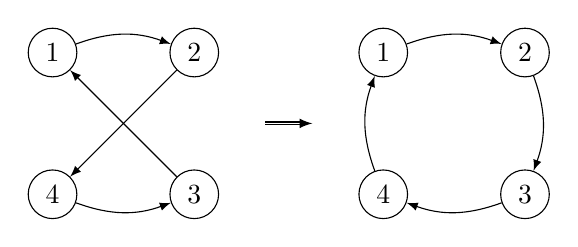
\begin{tikzpicture}[scale=0.6]
        \node[circle, draw, fill=white] (A0) at (0, 0) {1};
        \node[circle, draw, fill=white] (B0) at (3, 0) {2};
        \node[circle, draw, fill=white] (C0) at (3, -3) {3};
        \node[circle, draw, fill=white] (D0) at (0, -3) {4};
    
        \draw[-latex] (A0) to[bend left=20] (B0);
        \draw[-latex] (B0) -- (D0);
        \draw[-latex] (D0) to[bend right=20] (C0);
        \draw[-latex] (C0) -- (A0);
    
        \draw[double,-latex] (4.5,-1.5) -- (5.5,-1.5);
    
        \node[circle, draw, fill=white] (A1) at (7, 0) {1};
        \node[circle, draw, fill=white] (B1) at (10, 0) {2};
        \node[circle, draw, fill=white] (C1) at (10, -3) {3};
        \node[circle, draw, fill=white] (D1) at (7, -3) {4};
    
        \draw[-latex] (A1) to[bend left=20] (B1);
        \draw[-latex] (B1) to[bend left=20] (C1);
        \draw[-latex] (C1) to[bend left=20] (D1);
        \draw[-latex] (D1) to[bend left=20] (A1);
    \end{tikzpicture}
    \caption{Representation of an edge swap in 2-Opt.}
    \label{fig:2optMoves}
\end{figure}

A \textbf{swap} is a simple computation in which two edges are removed from a solution and replaced with a new pair of edges such that the newly obtained tour is a feasible solution.
Every swap is characterized by their \textbf{offset value}, which represent the quality of the swap and is calculated as the sum of the edges added minus the sum of the edges removed.
An offset is considered an optimizing offset only if its value is negative.
Each solution usually allows for a finite yet very large number of swaps, however 2-Opt only involves swaps that reduce the overall cost of the tour, or a swaps with an optimizing offset.
These swaps are referred to as \textbf{optimizing swaps} or \textbf{2-Opt moves}.

The key step in the 2-Opt algorithm consists in finding and choosing a combination of edges that allows for a 2-Opt move.
A simple approach consists in scanning all possible swaps and choose the first detected optimizing move.
Another approach consists in scanning all possible swaps like before, and selecting the swap with the best offset.
The first procedure has the advantage of being able to find a suitable swap faster, while the quality of the optimizing swaps is never considered.
As opposed to the first method, the second procedure takes longer to find swaps, but the swap selected is the one that reduces the cost of the solution the most.
In this project we implemented the second approach.

%Once the edges are swapped the total cost of the tour is recalculated, and if it is lower than the previous cost, the swap is integrated in the solution permanently, or until a better swap involving one of those two edges is found.
%This operation is iterated across all possible pairs of the tour, and is repeated until a time limit is reached, or no further improvements are possible (which involves checking all possible combinations many time, making it infeasible for real-life complex scenarios).
2-Opt can improve significantly a solution, while maintaining an acceptable computational complexity across the board.
Each iteration of 2-Opt is of $O(n^2)$ complexity, while the number of iterations depends both on the size and quality of the starting solution.
Its main limitation is the fact that due of it being a local search method, it usually gets stuck in a local minima, thus failing to find the best solution.

\begin{figure}[htbp]
    \begin{algorithm}[H]
        \TitleOfAlgo{\textbf{2-Opt}}
        \SetKwInOut{Input}{Input}
        % \SetKwInOut{Output}{Output}
        \Input{Graph $G(V,E)$ \newline Cost function $C: E \rightarrow \mathbb{R}$, where $c_{i,j} = C(e_{i,j})$ \newline A tour $T$ of $G$}
        % \Output{A better or equaly quality solution}
        \BlankLine
        %$finished \gets 0$ \\
        \While{true}{%$finished = 0$}{
            $s \gets$ swap with the lowest offset currently in $T$\\
            \eIf{offset($s$) $<$ 0}{
                apply $s$ to $T$
            }{
                break%$finished \gets 1$
            }
        }
    \end{algorithm}
    \caption{Pseudocode of the 2-Opt algorithm} 
    \label{fig:2OptPseudocode}
\end{figure}

\subsection{Implementation}

While in the Cost-Matrix approach the implementation is exactly the same as \figurename{ \ref{fig:2OptPseudocode}}, the same cannot be said for the other approaches.
As we saw in the previous chapter, the Base and AVX methods can be enhanced by using approximation techniques.

The function which finds the 2-Opt move with the lowest offset value is presented in two versions: one which computed the exact edge cost and another which uses approximations in the edge cost computation.
This is mandatory since by only using the approximated search some optimizing swaps might be missed, which is especially true when the offset of those swaps is close to zero.
Therefore an easy fix is to use the approximated search as long as the selected swap is optimizing when recomputed with the accurate methods.
Recomputing the offset at the proposal of any 2-Opt move is necessary, since the approximations might cause an unoptimizing swap to look like an optimizing one.

\begin{figure}[htbp]
    \begin{algorithm}[H]
        \TitleOfAlgo{\textbf{2-Opt with aproximated search}}
        \SetKwInOut{Input}{Input}
        % \SetKwInOut{Output}{Output}
        \Input{Graph $G(V,E)$ \newline Cost function $C: E \rightarrow \mathbb{R}$, where $c_{i,j} = C(e_{i,j})$ \newline A tour $T$ of $G$}
        % \Output{A better or equaly quality solution}
        \BlankLine
        $useApprox \gets$ True \\
        \While{true}{%$finished = 0$}{
            \eIf{useApprox}{
                $s \gets$ swap with the lowest offset currently in $T$ w.r.t. cost approximations \\
                recompute offset of $s$ using accurate cost functions
            }{
                $s \gets$ swap with the lowest offset currently in $T$
            }
            \eIf{offset($s$) $<$ 0}{
                apply $s$ to $T$
            }{
                \eIf{useApprox}{
                    $useApprox \gets$ False
                }{
                    break
                }
            }
        }
    \end{algorithm}
    \caption{Pseudocode of the 2-Opt algorithm adjusted to take advantage of aproximations for the Base and AVX versions} \label{fig:2OptPseudocodeApprox}
\end{figure}

% % In our implementation of 2-opt we decided to optimize heavily the method using AVX functions rather than multithreading 
% % (NOTE: check, and why AVX).
% The function that takes care of the application of the metaheuristic is apply2OptBestFix, to which we pass the solution to refine, and will apply the options selected at launch. 
% The heart of the algorithm lies in the two specular functions \_2OptBestFix and \_2OptBestFixApprox.
% The former will compute the exact edge cost when evaluating edge swaps, considering the actual distance between the points and delivering a more precise result, with the cost of a slower computation, especially for larger instances.
% The latter uses an approximated computation of the edges cost and provides a faster iteration time, with the counterpart of possibly producing slightly worse solutions. 
% These two methods will iterate over all possible pairs of edges in the tour and compute the potential decrease in total tour length if we were to apply the swap.
% The data regarding the best swap found so far, offset of the cost and the edges, is kept in the bestFix struct, to which we will compare each potential swap and which will be then implemented at the end of the iteration.


\subsection{3-Opt}

The 3-Opt metaheuristic is an extension of the 2-Opt algorithm, with the key difference that it is not limited to swaps involving just two edges, but instead considers swaps of up to three edges. This broader approach allows for a larger neighborhood of solutions to be explored, potentially enabling the algorithm to escape local minima that 2-Opt might not be able to overcome.

It is important to note, however, that while the solution space is expanded, escaping all local minima is not guaranteed and is generally not achievable with algorithms like this. The overall process is similar to 2-Opt, with the primary distinction being the number of nodes involved in each swap and the various configurations that these swaps can take.

The concepts of \textbf{swap}, \textbf{optimizing swap} and \textbf{offset value} remain the same as in the 2-Opt method, but they are extended to include three edges.
As shown in \figurename{ \ref{fig:3optMoves}}, the number of possible edge swaps increases significantly.
This not only raises the computational complexity due to the greater number of three-edge configurations, but also increases the asymptotic factor, which changes to $O(n^3)$ per iteration.

% As shown in figure \ref{fig:3optMoves}, starting from an existing solution, we iteratively consider three edges instead of two, and we change the way they are connected, looking for the one that has lower total cost.
% If a combination is found to improve the total cost of the solution then the swap is implemented, otherwise a different set of three edges is taken into consideration.
% Just as for 2-opt this iterative process can continue until a time limit is reached or until no more improving moves are possible.

\begin{figure}[htbp]
    \centering
    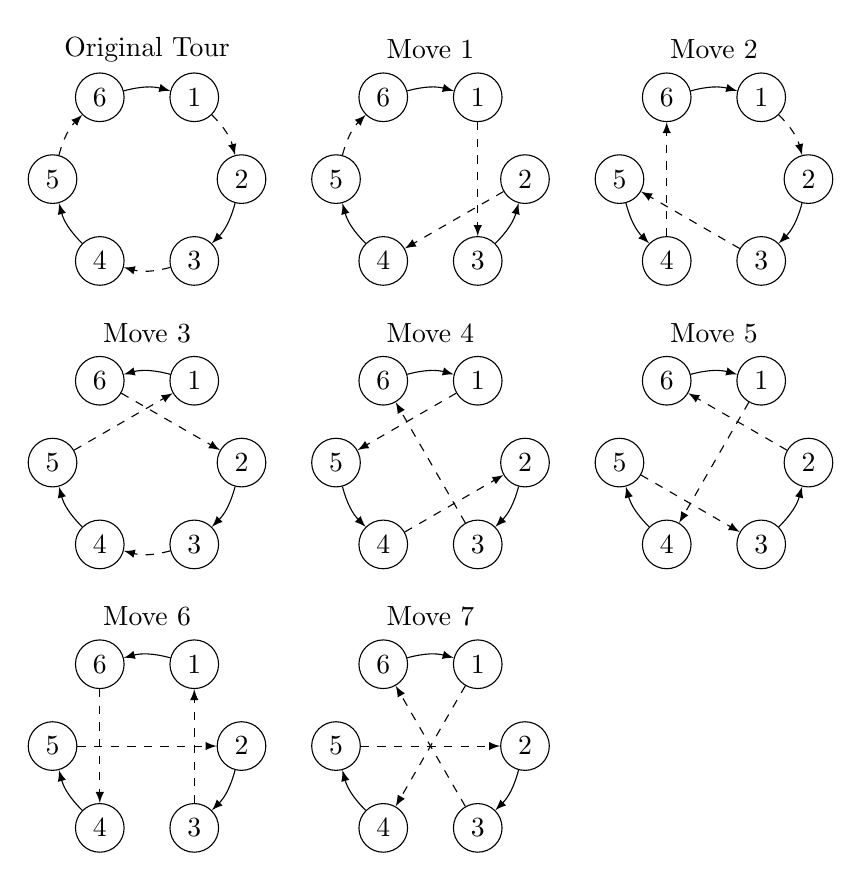
\begin{tikzpicture}[scale=0.6]
        \begin{scope}[shift={(0, 0)}]
            \node at (0, 2.75) {Original Tour};
        
            \node[circle, draw, fill=white] (N1) at ({60 * 2}:2) {6};
            \node[circle, draw, fill=white] (N2) at ({60 * 1}:2) {1};
            \node[circle, draw, fill=white] (N3) at ({60 * 0}:2) {2};
            \node[circle, draw, fill=white] (N4) at ({60 * 5}:2) {3};
            \node[circle, draw, fill=white] (N5) at ({60 * 4}:2) {4};
            \node[circle, draw, fill=white] (N6) at ({60 * 3}:2) {5};
        
            \draw[-latex] (N1) to[bend left=15] (N2);
            \draw[-latex,dashed] (N2) to[bend left=15] (N3);
            \draw[-latex] (N3) to[bend left=15] (N4);
            \draw[-latex,dashed] (N4) to[bend left=15] (N5);
            \draw[-latex] (N5) to[bend left=15] (N6);
            \draw[-latex,dashed] (N6) to[bend left=15] (N1);
        \end{scope}
    
        \begin{scope}[shift={(6, 0)}]
            \node at (0, 2.75) {Move 1};
        
            \node[circle, draw, fill=white] (N1) at ({60 * 2}:2) {6};
            \node[circle, draw, fill=white] (N2) at ({60 * 1}:2) {1};
            \node[circle, draw, fill=white] (N3) at ({60 * 0}:2) {2};
            \node[circle, draw, fill=white] (N4) at ({60 * 5}:2) {3};
            \node[circle, draw, fill=white] (N5) at ({60 * 4}:2) {4};
            \node[circle, draw, fill=white] (N6) at ({60 * 3}:2) {5};
        
            \draw[-latex] (N1) to[bend left=15] (N2);
            \draw[-latex,dashed] (N2) to (N4);
            \draw[-latex,dashed] (N3) to (N5);
            \draw[-latex] (N4) to[bend right=15] (N3);
            \draw[-latex] (N5) to[bend left=15] (N6);
            \draw[-latex,dashed] (N6) to[bend left=15] (N1);
        \end{scope}
    
        \begin{scope}[shift={(12, 0)}]
            \node at (0, 2.75) {Move 2};
        
            \node[circle, draw, fill=white] (N1) at ({60 * 2}:2) {6};
            \node[circle, draw, fill=white] (N2) at ({60 * 1}:2) {1};
            \node[circle, draw, fill=white] (N3) at ({60 * 0}:2) {2};
            \node[circle, draw, fill=white] (N4) at ({60 * 5}:2) {3};
            \node[circle, draw, fill=white] (N5) at ({60 * 4}:2) {4};
            \node[circle, draw, fill=white] (N6) at ({60 * 3}:2) {5};
        
            \draw[-latex] (N1) to[bend left=15] (N2);
            \draw[-latex,dashed] (N2) to[bend left=15] (N3);
            \draw[-latex] (N3) to[bend left=15] (N4);
            \draw[-latex,dashed] (N4) to (N6);
            \draw[-latex,dashed] (N5) to (N1);
            \draw[-latex] (N6) to[bend right=15] (N5);
        \end{scope}
    
        \begin{scope}[shift={(0, -6)}]
            \node at (0, 2.75) {Move 3};
        
            \node[circle, draw, fill=white] (N1) at ({60 * 2}:2) {6};
            \node[circle, draw, fill=white] (N2) at ({60 * 1}:2) {1};
            \node[circle, draw, fill=white] (N3) at ({60 * 0}:2) {2};
            \node[circle, draw, fill=white] (N4) at ({60 * 5}:2) {3};
            \node[circle, draw, fill=white] (N5) at ({60 * 4}:2) {4};
            \node[circle, draw, fill=white] (N6) at ({60 * 3}:2) {5};
        
            \draw[-latex,dashed] (N1) to (N3);
            \draw[-latex] (N2) to[bend right=15] (N1);
            \draw[-latex] (N3) to[bend left=15] (N4);
            \draw[-latex,dashed] (N4) to[bend left=15] (N5);
            \draw[-latex] (N5) to[bend left=15] (N6);
            \draw[-latex,dashed] (N6) to (N2);
        \end{scope}
    
        \begin{scope}[shift={(6, -6)}]
            \node at (0, 2.75) {Move 4};
        
            \node[circle, draw, fill=white] (N1) at ({60 * 2}:2) {6};
            \node[circle, draw, fill=white] (N2) at ({60 * 1}:2) {1};
            \node[circle, draw, fill=white] (N3) at ({60 * 0}:2) {2};
            \node[circle, draw, fill=white] (N4) at ({60 * 5}:2) {3};
            \node[circle, draw, fill=white] (N5) at ({60 * 4}:2) {4};
            \node[circle, draw, fill=white] (N6) at ({60 * 3}:2) {5};
        
            \draw[-latex] (N1) to[bend left=15] (N2);
            \draw[-latex,dashed] (N2) to (N6);
            \draw[-latex] (N3) to[bend left=15] (N4);
            \draw[-latex,dashed] (N4) to (N1);
            \draw[-latex,dashed] (N5) to (N3);
            \draw[-latex] (N6) to[bend right=15] (N5);
        \end{scope}
    
        \begin{scope}[shift={(12, -6)}]
            \node at (0, 2.75) {Move 5};
        
            \node[circle, draw, fill=white] (N1) at ({60 * 2}:2) {6};
            \node[circle, draw, fill=white] (N2) at ({60 * 1}:2) {1};
            \node[circle, draw, fill=white] (N3) at ({60 * 0}:2) {2};
            \node[circle, draw, fill=white] (N4) at ({60 * 5}:2) {3};
            \node[circle, draw, fill=white] (N5) at ({60 * 4}:2) {4};
            \node[circle, draw, fill=white] (N6) at ({60 * 3}:2) {5};
        
            \draw[-latex] (N1) to[bend left=15] (N2);
            \draw[-latex,dashed] (N2) to (N5);
            \draw[-latex,dashed] (N3) to (N1);
            \draw[-latex] (N4) to[bend right=15] (N3);
            \draw[-latex] (N5) to[bend left=15] (N6);
            \draw[-latex,dashed] (N6) to (N4);
        \end{scope}
    
        \begin{scope}[shift={(0, -12)}]
            \node at (0, 2.75) {Move 6};
        
            \node[circle, draw, fill=white] (N1) at ({60 * 2}:2) {6};
            \node[circle, draw, fill=white] (N2) at ({60 * 1}:2) {1};
            \node[circle, draw, fill=white] (N3) at ({60 * 0}:2) {2};
            \node[circle, draw, fill=white] (N4) at ({60 * 5}:2) {3};
            \node[circle, draw, fill=white] (N5) at ({60 * 4}:2) {4};
            \node[circle, draw, fill=white] (N6) at ({60 * 3}:2) {5};
        
            \draw[-latex,dashed] (N1) to (N5);
            \draw[-latex] (N2) to[bend right=15] (N1);
            \draw[-latex] (N3) to[bend left=15] (N4);
            \draw[-latex,dashed] (N4) to (N2);
            \draw[-latex] (N5) to[bend left=15] (N6);
            \draw[-latex,dashed] (N6) to (N3);
        \end{scope}
    
        \begin{scope}[shift={(6, -12)}]
            \node at (0, 2.75) {Move 7};
        
            \node[circle, draw, fill=white] (N1) at ({60 * 2}:2) {6};
            \node[circle, draw, fill=white] (N2) at ({60 * 1}:2) {1};
            \node[circle, draw, fill=white] (N3) at ({60 * 0}:2) {2};
            \node[circle, draw, fill=white] (N4) at ({60 * 5}:2) {3};
            \node[circle, draw, fill=white] (N5) at ({60 * 4}:2) {4};
            \node[circle, draw, fill=white] (N6) at ({60 * 3}:2) {5};
        
            \draw[-latex] (N1) to[bend left=15] (N2);
            \draw[-latex,dashed] (N2) to (N5);
            \draw[-latex] (N3) to[bend left=15] (N4);
            \draw[-latex,dashed] (N4) to (N1);
            \draw[-latex] (N5) to[bend left=15] (N6);
            \draw[-latex,dashed] (N6) to (N3);
        \end{scope}
    
    \end{tikzpicture}
    \caption{3-Opt available moves}
    \label{fig:3optMoves}
\end{figure}

\subsection{Performance}

As expected, the quality of the solutions found by the 3-Opt algorithm consistently surpasses that of 2-Opt.
However, the time required by the two algorithms differs significantly: while 2-Opt completes the optimization of a NN generated solution in under a second, the 3-Opt algorithm takes over a minute to fully optimize the same solution.

\begin{figure}[htbp]
	\centering
	\begin{tikzpicture}
        \begin{axis}[
            xlabel={Cost Ratio},
            xmin=1, xmax=1.082,
            ymin=0, ymax=70,
            xtick={},
            ytick=\empty,
            legend style={at={(0.98,0.02)},anchor=south east,legend columns=1},
			legend cell align={left},
            %ymajorgrids=true,
            xmajorgrids=true,
            grid style=dashed,
        ]
        
        \addplot[Blue,mark=square,mark size=1.5] table[x=ones,y=idx, col sep=semicolon] {csv/23opt.csv}; 
        \addplot[Red,mark=o,mark size=1.5] table[x=2opt,y=idx, col sep=semicolon] {csv/23opt.csv};
        \addplot[Green,mark=triangle,mark size=1.5] table[x=3opt,y=idx, col sep=semicolon] {csv/23opt.csv}; 
        \addlegendentry{Optimal} 
        \addlegendentry{2-Opt}
        \addlegendentry{3-Opt}
            
        \end{axis}
    \end{tikzpicture}
	\caption{Performance comparison between different tenure sizes} \label{fig:23OptPerformance}
\end{figure}

\section{Tabu Search}

Tabu search is a metaheuristic designed to escape local minima.
The key idea is to avoid revisiting solutions that are known not to lead to the global optimum.

Let's assume we already have a refined solution and have reached a local minimum using the 2-Opt algorithm; we'll call this solution $x_k$.
Attempting to refine it further will not yield any improvement, as $x_k$ contains no 2-Opt moves, having been fully optimized by 2-Opt.
Tabu Search addresses this situation by accepting a \textit{bad} move; in other words, it performs a swap even if it results in a positive offset\footnote{A swap with a positive offset is a swap that increases the overall cost of the solution}.

Therefore, a new tour, $x_{k+1}$, is produced in the hope that applying 2-Opt again will yield a better solution than $x_k$.
However, there's a significant chance that the local search algorithm will revert from $x_{k+1}$ back to $x_k$, ending up in the same local minimum.
To avoid this, Tabu Seach uses a list called \textbf{tenure} which records the swaps made to escape a local minima.
This tenure list acts as a set of \textit{forbidden swaps}, ensuring that 2-Opt cannot perform swaps that are included in this data structure.

There are additional considerations regarding the tenure, particularly its size and contents.
Intuitively, the size of this list should be limited, otherwise, it might block too many edges, causing the optimization to become stuck with no swaps allowed.
This particular aspect of the tenure will be explored in the next subsection, in which multiple tenure sizes will be compared.
When the list is full, newly introduced \textit{forbidden swaps} replace the oldest elements in the tenure.

Another potential improvement regards a detection mechanism on whether the local minima has been escaped or not: by checking if 2-Opt made any improvements on the solution, even while avoiding \textit{forbidden moves}, it is possible to have a rough estimation on wether or not the local optima point has been escaped or not.
Upon detecting a potential escape, removing the oldest element from the tenure in hope of having actually escaped of the local minima.
% This size is called \textit{NOT TENURE}, and could be a fixed amount or it could be adaptive depending on the instance of the problem we are approaching.
% When the list is full, we start replacing the edges in it starting from the older ones.

It's imperative for this procedure to work to its fullest to always keep a copy of the best solution found throughout its execution between all working threads.
This process continues until some termination condition is reached.
As for the other metaheuristic presented in this project, the termination condition is a time limit.

\subsection{Edge locking implementation}

The mechanism in which \textit{forbidden swaps} are avoided can be difficult in its design.
In this project, we implemented the \textit{forbidden swaps} by preventing a single edge of such swaps from being used in a 2-Opt move.
We refer to this as the \textbf{edge locking procedure}.
For each \textit{forbidden swap} we lock in place a single edge, which is chosed at random between the two edges introduced by the swap.
Locking both edges will effectively prevent any improvement from any 2-Opt implementation, since the remaining part of the solution in already optimized.

In our implementation 2-Opt is an external method called from the tabu function, and we needed to figure out a way to prevent it to perform swaps which involve edges locked in the tenure.
To this end we exploited the cost cache implementation by setting the cost of locked edges to $-\infty$.

Let's consider a swap $s$ involving two \textit{current} edges, $e_{a,b}$, $e_{c,d}$, which are part of the current solution, and two \textit{alternative} edges, $e_{a,c}$, $e_{b,d}$, which are the edges that would replace $e_{a,b}$ and $e_{c,d}$.
The offset of $s$ is defined as
\[
    \text{offset}(s) = [c(e_{a,c}) + c(e_{b,d})] - [c(e_{a,b}) + c(e_{c,d})]
\]
In 2-Opt $s$ has a chance of being applied to a solution only if offset$(s)<0$.
If $e_{a,b}$ is a locked edge than $c(e_{a,b})=-\infty$, as defined in the cost cache.
This means that offset$(s) = [c(e_{a,c}) + c(e_{b,d})] - [-\infty + c(e_{c,d})] = \infty > 0$, so swap $s$ will not be applied by 2-Opt.
The same reasoning applies if $e_{c,d}$ is the locked edge.

Therefore we can apply the 2-Opt procedure in a way which respects the locked edges without any additional effort.
This edge locking mechanic can be used if 3-Opt is used as local search method instead, altough it is not guaranteed to be as effective.

\begin{figure}[htbp]
    \begin{algorithm}[H]
        \TitleOfAlgo{\textbf{Tabu Search}}
        \SetKwInOut{Input}{Input}
        \SetKwInOut{Output}{Output}
        \Input{Graph $G(V,E)$ \newline Cost function $c$ \newline A tour $T$ of $G$ \newline Size of the tenure $l_{size}$}
        \Output{A tour $T_{best}$ where $c(T_{best}) \leq c(T)$}
        \BlankLine
        $L \gets [\;]$\\
        $T \gets$ 2-Opt($T$)\\
        $T_{best} \gets T$\\
        \While{time limit is not reached}{
            \BlankLine
            select at random edges $e_0, e_1 \in T$ that are suitable to perform a swap in $T$\\
            \lIf{random$\{0,1\}$ = 1}{
                $e_0 \leftrightarrows e_1$
            }
            $L \gets L \cup \{e_0\}$\\
            \lIf{$|L| > l_{size}$}{
                $L \gets L \backslash \{l_0\}$, where $l_0$ is the oldest element in $L$
            }
            \BlankLine
            $T_{new} \gets$ 2-Opt($T$)\\
            \While{$c(T_{new}) \neq c(T)$}{
                $T \gets T_{new}$\\
                \lIf{$c(T) < c(T')$}{$T' \gets T$}
                $L \gets L \backslash \{l_0\}$\\
                $T_{new} \gets$ 2-Opt($T$)
            }
        }
        \Return $T_{best}$
    \end{algorithm}
    \caption{Pseudocode of the Tabu Search algorithm. The Cost-cache related part are implicit as they are performed according to the tenure $L$} \label{fig:tabuPseudocode}
\end{figure}

% \subsection{Implementation}
% TabuSearch is the main method that manages the execution of the tabu algorithm.
% After receiving the solution, it sets the tenure size, which is implemented as an array of struct Edge, accordingly to input.
% We implemented a check on the value passed for this parameter: if we don't receive any specific size the default value of 2 is set; if we receive a value that is larger of equal to the amount of nodes in 
% the instace an error is thrown, since this will lead to the algorithm getting stuck; and lastly, if the value is larger than the 97\% of the 
% number of nodes a warning message will indicate the possibility of the method getting stuck and not respecting the time limit.
% After this, the function runTabu is launched whithin the threads and takes care of the execution of the metaheuristic, starting from the current best solution (CHECK IF ITS THE PASSED SOLUTION).
% The main loop that keeps going until the time limit consists in selecting two random edges in the solution, swapping them and locking one of the two by inserting it into the tenure.
% Once we have done that 2-opt is launched to refine the solution, and we keep relaunching it until there are no further improving moves possible, freeing the oldest element in the tenure before relaunching it every time.
% A counter is implemented to keep track of the number of iteration in which the method does not find a solution 
% that is better than the best one found so far, and when it reaches a threshold the working solution of the thread is resetted back to the best one.

\subsection{Performance}

To study the performance of the Tabu Search algorithm we implemented we must first choose a key hyperparameter: the \textbf{tenure size}.
We chose three different values which are compared in \figurename{ \ref{fig:tabuParmTune}}.

\begin{figure}[htbp]
	\centering
	\begin{tikzpicture}
        \begin{axis}[
            xlabel={Cost Ratio},
            %ylabel={Iterations/s Ratio},
            xmin=1, xmax=1.03,
            ymin=0, ymax=74,
            xtick={},
            ytick=\empty,
            legend style={at={(0.98,0.02)},anchor=south east,legend columns=1},
			legend cell align={left},
            %ymajorgrids=true,
            xmajorgrids=true,
            grid style=dashed,
        ]
        
        \addplot[Blue,mark=square,mark size=1.5] table[x=p1cost,y=idx, col sep=semicolon] {csv/tabu.csv}; 
        \addplot[Red,mark=o,mark size=1.5] table[x=p2cost,y=idx, col sep=semicolon] {csv/tabu.csv};
        \addplot[Green,mark=triangle,mark size=1.5] table[x=p3cost,y=idx, col sep=semicolon] {csv/tabu.csv}; 
        \addlegendentry{Tenure size = 1} 
        \addlegendentry{Tenure size = 2}
        \addlegendentry{Tenure size = 3}
            
        \end{axis}
    \end{tikzpicture}
	\caption{Performance comparison between different tenure sizes.} \label{fig:tabuParmTune}
\end{figure}

As shown in the graph, the tenure size value which consistently gave the best results was 1.
This is strictly dependent on our implementation of the Tabu Search method, since other implementations might use different edge locking mechanics as well as different local search method.
Still this result is a bit unexpected, since we were expecting to see a linear correlation between the tenure size and the size of the instance, with larger instances favoring larger tenures.
However, as stated above, this result is specific to this implementation, so there might be some opportunity to optimize this algorithm, albeit we didn't manage to find it.

\begin{figure}[htbp]
	\centering
	\begin{tikzpicture}
        \begin{axis}[
            ylabel={Iterations/s Ratio},
            xlabel={Sorted instances},
            xmin=0, xmax=74,
            ymin=1, ymax=1.1,
            ytick={},
            xtick=\empty,
            legend style={at={(0.02,0.98)},anchor=north west,,legend columns=1},
			legend cell align={left},
            ymajorgrids=true,
            %xmajorgrids=true,
            grid style=dashed,
        ]
        
        \addplot[Blue,mark=square,mark size=1.5] table[y=p1iter,x=idx, col sep=semicolon] {csv/tabu.csv};
        \addplot[Red,mark=o,mark size=1.5] table[y=p2iter,x=idx, col sep=semicolon] {csv/tabu.csv};
        \addplot[Green,mark=triangle,mark size=1.5] table[y=p3iter,x=idx, col sep=semicolon] {csv/tabu.csv};
        \addlegendentry{Tenure size = 1}
        \addlegendentry{Tenure size = 2}
        \addlegendentry{Tenure size = 3} 
            
        \end{axis}
    \end{tikzpicture}
	\caption{Comparison between tabu search parameters and iteration count.} \label{fig:tabuIters}
\end{figure}

In order to check for other causes to this behavior we also compared the speed of each tenure size configuration, as shown by \figurename{ \ref{fig:tabuIters}}.
The configuration with tenure size set to 1 is the one which displayed the highest number of iterations per second, altough the speed difference is too small to actually arise suspitions.

\begin{figure}[htbp]
	\centering
	\begin{tikzpicture}
        \begin{axis}[
            xlabel={Cost Ratio},
            %ylabel={Iterations/s Ratio},
            xmin=1, xmax=1.082,
            ymin=0, ymax=74,
            xtick={},
            ytick=\empty,
            legend style={at={(0.98,0.02)},anchor=south east,legend columns=1},
			legend cell align={left},
            %ymajorgrids=true,
            xmajorgrids=true,
            grid style=dashed,
        ]
        
        \addplot[Blue,mark=square,mark size=1.5] table[x=startcost,y=idx, col sep=semicolon] {csv/tabu.csv}; 
        \addplot[Red,mark=o,mark size=1.5] table[x=finalcost,y=idx, col sep=semicolon] {csv/tabu.csv};
        \addplot[Green,mark=triangle,mark size=1.5] table[x=optimalcost,y=idx, col sep=semicolon] {csv/tabu.csv}; 
        \addlegendentry{Initial Cost} 
        \addlegendentry{Final Cost}
        \addlegendentry{Optimal Cost}
            
        \end{axis}
    \end{tikzpicture}
	\caption{Performance of with tenure size set to 1.} \label{fig:tabuCost}
\end{figure}

\figurename{ \ref{fig:tabuCost}} shows the gap in percentage between the optimal solution, an initial solution found using NN and 2-Opt and the output of the Tabu Search procedure.
Tabu Search managed to optimize every initial solution to a better one, sometimes even reaching optimality.



\newpage
\section{Variable Neighborhood Search}

The Variable Neighborhood Search (VNS) is a metaheuristic method introduced by Mladenović and Hansen in 1997\cite{vnsWikipedia}.
It aims to solve combinatorial and global optimization problems by systematically changing the neighborhood structures during the search process.
VNS explores different neighborhoods of the current solution, and if a better solution is found, the search moves to this new solution.
The method involves two main phases: a descent phase, which focuses on finding a local optimum by exploring the current neighborhood, and a perturbation phase, which helps escape local minima by perturbing the solution to explore new areas of the solution space.

\begin{figure}[htbp]
    \begin{algorithm}[H]
        \TitleOfAlgo{\textbf{Variable Neighborhood Search}}
        \SetKwInOut{Input}{Input}
        \SetKwInOut{Output}{Output}
        \Input{Graph $G(V,E)$ \newline Cost function $c$ \newline A tour $T$ of $G$ \newline Perturbation magnitude interval $[p_{min},p_{max}]$}
        \Output{A tour $T_{best}$ where $c(T_{best}) \leq c(T)$}
        \BlankLine
        $T \gets$ 2-Opt($T$)\\
        $T_{best} \gets T$\\
        \While{time limit is not reached}{
            $p \gets$ random in range $[p_{min}, p_{max}]$\\
            $T \gets$ \textbf{Perturb}($T$, $p$)\\
            $T \gets$ 2-Opt($T$)\\
            \lIf{$c(T) \leq c(T_{best})$}{$T_{best} \gets T$}
        }
        \Return $T_{best}$
    \end{algorithm}
    \caption{Pseudocode of the VNS algorithm} \label{fig:vnsPseudocode}
\end{figure}

We implemented this algorithm in a very simple manner, since it does not require any particular data structure like the tenure in Tabu Search.
Its implementation consists of a perturbation part and a optimization part.
The latter simply uses the 2-Opt algorithm to explore the neighborhood, taking advantage of all the efficiency optimizations implemented in 2-Opt.
The 3-Opt algorithm works just as well here, altough its increased computational cost led us to just using 2-Opt.

% Variable Neighborhood Search (VNS) is a technique that explores various neighborhoods within the solution space to seek a potentially optimal solution to a problem.
% This metaheuristic closely resembles Tabu Search at a high level of abstraction.
% It begins with a feasible solution and, using a local search algorithm, explores its neighborhood to identify the best solution within that vicinity before moving on to another neighborhood.
% The aim of VNS is to explore different portions of the solution space with the hope of eventually finding the neighborhood of the optimal solution.
% The differnce with Tabu search lies in its behavior when incurring into local minima.
% Instead of trying to escape the neigborhood by perfoming worseining moves and locking parts of it in place, VNS tries to change the solution just enough to escape.

% While we do this process we keep track of the best solution found so far, and we replace it when a new neighborhood reveals a better minima.
% In TSP, to explore the neighborhood of a solution we used the 2-Opt algorithm, while using the 3-Opt extension can be done as well.
% Doing this allows us change the space in which we search for the solution using local search maintaining most of the existing tour untouched.

\begin{figure}[htbp]
    \centering
    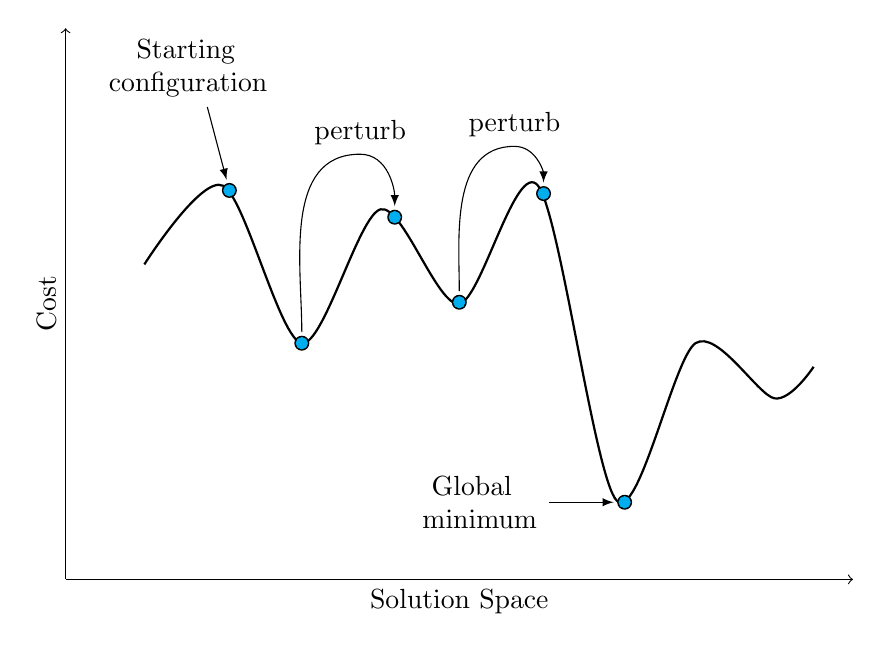
\begin{tikzpicture}[scale=1]
        \draw[->] (0,0) -- node[below] {Solution Space} (10,0);
        \draw[->] (0,0) -- node[above,sloped] {Cost} (0,7);
    
        \coordinate (A) at (1, 4);
        \coordinate (B) at (2, 5);
        \coordinate (C) at (3, 3);
        \coordinate (D) at (4, 4.7);
        \coordinate (E) at (5, 3.5);
        \coordinate (F) at (6, 5);
        \coordinate (G) at (7, 1);
        \coordinate (H) at (8, 3);
        \coordinate (I) at (9, 2.3);
        \coordinate (J) at (9.5, 2.7);
    
        \draw[black,thick] plot [smooth] coordinates {(A) (B) (C) (D) (E) (F) (G) (H) (I) (J)};
    
        \coordinate (P1) at (2.08,4.94);
        \coordinate (P2) at (3,3);
        \coordinate (P3) at (4.18,4.6);
        \coordinate (P4) at (5,3.52);
        \coordinate (P5) at (6.07,4.9);
        \coordinate (P6) at (7.1,0.98);

		\coordinate (P2_3) at (3.74,5.4);
		\coordinate (P4_5) at (5.7,5.5);

		\coordinate (SP) at (1.8,6);
		\coordinate (GB) at (6,0.98);
        
        % Draw jump arrows
        \draw[black,-latex,shorten <=4pt,shorten >=4pt] (P2) to[out=90, in=180] (P2_3) to[out=0, in=90] (P3);
        \node[above] at (P2_3) {perturb};
        \draw[black,-latex,shorten <=4pt,shorten >=4pt] (P4) to[out=90, in=180] (P4_5) to[out=0, in=90] (P5);
        \node[above] at  (P4_5) {perturb};
        
        % Comment arrows
        \draw[black,-latex,shorten >=4pt] (SP) -- (P1);
        \node[above,yshift=0,text width=25mm] at (SP) {\quad Starting \quad configuration};
        \draw[black,-latex,shorten <=4pt,shorten >=4pt] (GB) -- (P6);
        \node[left,xshift=13,yshift=0,text width=18mm] at (GB) {\ Global \ minimum};
        
    
        % Draw points
        \foreach \point in {P1,P2,P3,P4,P5,P6}  {
            \filldraw [black] (\point) circle (2.5pt);
            \filldraw [cyan] (\point) circle (2pt);
        }
    
    \end{tikzpicture}
    \caption{Iteration process of VNS}
    \label{fig:vns}
\end{figure}

% VNS balances exploration (through varying neighborhood structures) and exploitation (through local search) to efficiently search the solution space.
% The number of edges that we decide to swap can be dependent of the size of the instance, if we were working on a small instance, e.g. 
% ~50 nodes, swapping more than ten edges could result in a change way too big of the starting solution, worsening it unnecessarily.

\subsection{Perturbation implementation}

\begin{figure}[htbp]
    \begin{algorithm}[H]
        \TitleOfAlgo{\textbf{VNS Perturbation}}
        \SetKwInOut{Input}{Input}
        \SetKwInOut{Output}{Output}
        \Input{A tour $T$ of $G$ as an array of indices \newline Perturbation magnitude $p$}
        \Output{A perturbated tour $T_p$}
        \BlankLine
        $L \gets [\;]$\\
        \For{$i \in \{0,1,\dots,p-1\}$}{
            \BlankLine
            $r \gets $ random in range $[0,|T|)$\\
            \lWhile{$r \in L$}{$r \gets $ random in range $[0,|T|)$}
            $L \gets L \cup \{r\}$
        }
        \BlankLine
        $b \gets T[L[0]]$\\
        \BlankLine
        \For{$i \in \{0,1,\dots,p-2\}$}{
            \BlankLine
            $T[L[i]] \gets T[L[i+1]]$
        }
        \BlankLine
        $T[L[p-1]] \gets b$\\
        \BlankLine
        \Return $T$
    \end{algorithm}
    \caption{Pseudocode of the Perturbation procedure implemented in VNS} \label{fig:vnsPerturbPseudocode}
\end{figure}

The \textbf{perturbation} is the procedure in which the solution is changed to escape the local minima.
It's very important to choose a suitable perturbation method for the selected local neighborhood search algorithm.
It has to be able to modify the solution enough to escape local optimal points while not modifying it too much as to land in a completely different state.

In the literature, the perturbation does not have a strict definition, instead it depends on the optimization problem and the local search method chosen while still retaining some freedom for its implementation.
Our implementation involves swapping nodes at random in the solution array.
The process consists in the following steps:
\begin{enumerate}
    \item Select a the permutation magnitude, which is the number of nodes that will change their position inside the solution array; this choice is made at random between a defined interval.
    \item Choose at random the nodes which will be affected by the perturbation, with particular care to not select the same element twice.
    \item According to the order in which nodes were selected for the perturbation, move them in a circular way between each other in the solution array.
\end{enumerate}

% \subsection{Implementation(? Maybe talk specifics on how kick works)}
% For the implementation of VNS we have the main function VariableNeighborhoodSearch which is in charge of managing the various threads initialization 
% and coordination, along with the time management in order to maintain the execution of the algorithm within the time limit provided in input.
% Inside the threads we will run parallely the function runVns, which performs the actual algorithm.
% The loop inside the threads will start by taking the passed solution and perform a repeating cycle of 2-opt operations and kicks. 2-opt is in charge 
% of searching the local space of the solution, while the kick will ensure a traslation to a neighboring search space.
% For the kick we implemented a swap of a dynamically chosen amount of edges. We did this to adapt to different scales of instances, since a fixed 
% amount of edges swaps (e.g. five each time) could result in a non-effective enough of a neighborhood change for large instances. All the edges involved in the kick are selected randomly.
% After each execution of 2-opt the obtained solution will be compared with the saved best solution found so far, and, if the cost is improved, the 
% best solution gets updated. Note that the best solution is shared among the threads and its access is managed by mutex.

\subsection{Performance}

Our implementation of VNS requires tuning only one hyperparameter: the perturbation magnitude interval.
Each time that we apply a perturbation a number within the interval is picked at random, and it represents the amount of nodes in the solution array that are getting swapped.

In order to find the best possible variable we tested the algorithm by running it in different configurations multiple times.
The intervals we chose to test were: [4,4], [5,5], [5,10], [5,20], [5,40] and [20,40].
As shown by \figurename{ \ref{fig:vnsParmTune}}, the best overall intervals were the [5,5] and the [5,10] with a slight advantage of the latter.

\begin{figure}[htbp]
	\centering
	\begin{tikzpicture}
        \begin{axis}[
            xlabel={Cost Ratio},
            xmin=1, xmax=1.015,
            ymin=0, ymax=74,
            xtick={1,1.005,1.01,1.015},
            xticklabel style={/pgf/number format/fixed,/pgf/number format/precision=4},
            ytick=\empty,
            legend style={at={(0.98,0.02)},anchor=south east,legend columns=1},
			legend cell align={left},
            xmajorgrids=true,
            grid style=dashed,
        ]
        
        \addplot[Blue,mark=square,mark size=1.5] table[x=p4_4cost, y=idx, col sep=semicolon] {csv/vns.csv}; 
        \addplot[Red,mark=o,mark size=1.5] table[x=p5_5cost, y=idx, col sep=semicolon] {csv/vns.csv};
        \addplot[Green,mark=triangle,mark size=1.5] table[x=p5_10cost, y=idx, col sep=semicolon] {csv/vns.csv};
        \addplot[Purple,mark=star,mark size=1.5] table[x=p5_20cost, y=idx, col sep=semicolon] {csv/vns.csv};
        \addplot[Dandelion,mark=otimes,mark size=1.5] table[x=p5_40cost, y=idx, col sep=semicolon] {csv/vns.csv};
        \addplot[Black,mark=diamond,mark size=1.5] table[x=p20_40cost, y=idx, col sep=semicolon] {csv/vns.csv};
        \addlegendentry{[ 4, 4]}
        \addlegendentry{[ 5, 5]}
        \addlegendentry{[ 5,10]}
        \addlegendentry{[ 5,20]}
        \addlegendentry{[ 5,40]}
        \addlegendentry{[20,40]}
            
        \end{axis}
    \end{tikzpicture}
	\caption{Performance comparison between different perturbation magnitude intervals} \label{fig:vnsParmTune}
\end{figure}

\begin{figure}[htbp]
	\centering
	\begin{tikzpicture}
        \begin{axis}[
            ylabel={Iterations/s Ratio},
            xlabel={Sorted instances},
            xmin=0, xmax=74,
            ymin=1, ymax=18,
            ytick={1,2,4,6,8,10,12,14,16},
            xtick=\empty,
            legend style={at={(0.02,0.98)},anchor=north west,,legend columns=1},
			legend cell align={left},
            ymajorgrids=true,
            grid style=dashed,
        ]
        
        \addplot[Blue,mark=square,mark size=1.5] table[y=p4_4iter, x=idx, col sep=semicolon] {csv/vns.csv}; 
        \addplot[Red,mark=o,mark size=1.5] table[y=p5_5iter, x=idx, col sep=semicolon] {csv/vns.csv};
        \addplot[Green,mark=triangle,mark size=1.5] table[y=p5_10iter, x=idx, col sep=semicolon] {csv/vns.csv};
        \addplot[Purple,mark=star,mark size=1.5] table[y=p5_20iter, x=idx, col sep=semicolon] {csv/vns.csv};
        \addplot[Dandelion,mark=otimes,mark size=1.5] table[y=p5_40iter, x=idx, col sep=semicolon] {csv/vns.csv};
        \addplot[Black,mark=diamond,mark size=1.5] table[y=p20_40iter, x=idx, col sep=semicolon] {csv/vns.csv};
        \addlegendentry{[ 4, 4]}
        \addlegendentry{[ 5, 5]}
        \addlegendentry{[ 5,10]}
        \addlegendentry{[ 5,20]}
        \addlegendentry{[ 5,40]}
        \addlegendentry{[20,40]}
            
        \end{axis}
    \end{tikzpicture}
	\caption{Comparison between VNS parameters in speed.} \label{fig:vnsIters}
\end{figure}

To investigate these differences in performance we also compared the speed that each configuration yielded.
\figurename{ \ref{fig:vnsIters}} highlights the large gap in speed between each of the selected intervals, with smaller intervals, and with smaller bounds, running faster compared to larger ones.
This behavior is to be expected since a higher perturbation magnitude causes solutions to be of overall worse quality compared to solutions affected by lighter perturbation.
Of course the higher the quality of a solution after a perturbation, the less time 2-Opt will take to optimize it, which explains the difference in speed between each configuration.

However there is likely more to this behavior than simple execution speed.
For istance, we can hypothesize that perturbations of a magnitude that is too high could be causing the algorithm to skip over high quality areas in solution space.
The opposite is true as well: a perturbation that isn't strong enough problably does not manage to escape local minima neighborhoods as it was the case with the [4,4] interval.

Likely, to find a good hyperparameter that can be of the right magnitude to both prevent skipping over the optimal solution neighborhood but still ensure escaping local minimas, a better criterion shoud be applied. 
%A way to obtain the best from both phenomemon likely lies in a different criterion in which the magnitude in picked inside the interval.
In our implementations we selected the size of the perturbation by picking an element in the chosen interval uniformly at random.
Switching from that to a different distribution, like an exponential distribution, would allow smaller perturbation to be performed more often than larger ones.
This could result in a behavior that is overall fast due to the smaller average size of perturbation, but still able to escape larger valleys in solution space using rare but large perturbations.

\begin{figure}[htbp]
	\centering
	\begin{tikzpicture}
        \begin{axis}[
            xlabel={Cost Ratio},
            xmin=1, xmax=1.082,
            ymin=0, ymax=74,
            xtick={},
            ytick=\empty,
            legend style={at={(0.98,0.02)},anchor=south east,legend columns=1},
			legend cell align={left},
            xmajorgrids=true,
            grid style=dashed,
        ]
        
        \addplot[Blue,mark=square,mark size=1.5] table[x=startcost,y=idx, col sep=semicolon] {csv/vns.csv}; 
        \addplot[Red,mark=o,mark size=1.5] table[x=finalcost,y=idx, col sep=semicolon] {csv/vns.csv};
        \addplot[Green,mark=triangle,mark size=1.5] table[x=optimalcost,y=idx, col sep=semicolon] {csv/vns.csv}; 
        \addlegendentry{Initial Cost} 
        \addlegendentry{Final Cost}
        \addlegendentry{Optimal Cost}
            
        \end{axis}
    \end{tikzpicture}
	\caption{Performance of with perturbation interval set to [5,10]} \label{fig:vnsCost}
\end{figure}


\newpage

\section{Simulated Annealing}

\begin{figure}[htbp]
    \centering
    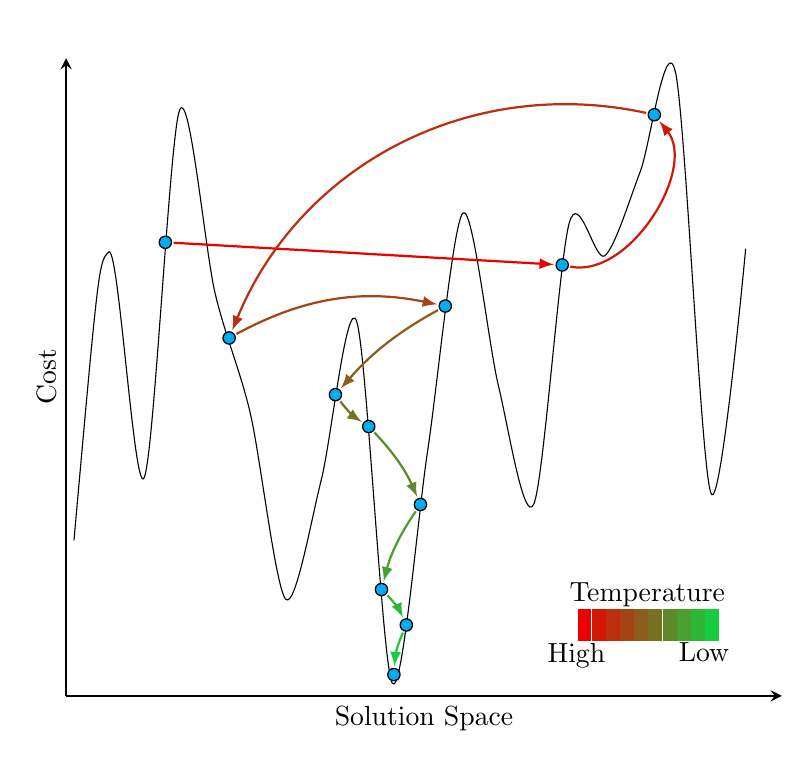
\begin{tikzpicture}
		[scale=0.9,shorten <=3pt,shorten >=3pt,>=stealth]

        \draw[thick,->,shorten <=0pt,shorten >=0pt,>=stealth] (-0.1,1) -- node[below] {Solution Space} (10,1);
        \draw[thick,->,shorten <=0pt,shorten >=0pt,>=stealth] (-0.1,1) -- node[above,sloped] {Cost} (-0.1,10);

		\draw[black,] plot [smooth] coordinates {(0,3.076)(0.5,7.263)(1,4.076)(1.5,9.263)(2,6.689)(2.5,4.981)(3,2.362)(3.5,4.046)(4,6.282)(4.5,1.183)(5,4.45)(5.5,7.813)(6,5.376)(6.5,3.708)(7,7.675)(7.5,7.209)(8,8.394)(8.5,9.791)(9,3.856)(9.5,7.428)};

        \coordinate (P1) at (1.3,7.4);
        \coordinate (P2) at (6.9,7.08);
        \coordinate (P3) at (8.2,9.2);
        \coordinate (P4) at (2.2,6.05);
        \coordinate (P5) at (5.25,6.5);
        \coordinate (P6) at (3.7,5.25);
        \coordinate (P7) at (4.17,4.8);
        \coordinate (P8) at (4.9,3.7);
        \coordinate (P9) at (4.35,2.5);
        \coordinate (P10) at (4.7,2);
        \coordinate (P11) at (4.525,1.3);
              
        \foreach \point in {P1,P2,P3,P4,P5,P6,P7,P8,P9,P10,P11}  {
            \filldraw [black] (\point) circle (2.5pt);
            \filldraw [cyan] (\point) circle (2pt);
        }

        \definecolor{C1}{RGB}{235, 0, 0}
        \definecolor{C2}{RGB}{211, 23, 7}
        \definecolor{C3}{RGB}{188, 46, 14}
        \definecolor{C4}{RGB}{164, 68, 20}
        \definecolor{C5}{RGB}{141, 91, 27}
        \definecolor{C6}{RGB}{118, 114, 34}
        \definecolor{C7}{RGB}{94, 137, 41}
        \definecolor{C8}{RGB}{71, 160, 48}
        \definecolor{C9}{RGB}{47, 182, 54}
        \definecolor{C10}{RGB}{24, 205, 61}

		\draw[-latex,color=C1,thick] (P1) to (P2);
		\draw[-latex,color=C2,thick] (P2) to[bend right=70] (P3);
		\draw[-latex,color=C3,thick] (P3) to[bend right=40] (P4);
		\draw[-latex,color=C4,thick] (P4) to[bend left=20] (P5);
		\draw[-latex,color=C5,thick] (P5) to[bend right=10] (P6);
		\draw[-latex,color=C6,thick] (P6) to[bend right=10] (P7);
		\draw[-latex,color=C7,thick] (P7) to[bend left=10] (P8);
		\draw[-latex,color=C8,thick] (P8) to[bend right=10] (P9);
		\draw[-latex,color=C9,thick] (P9) to[bend left=10] (P10);
		\draw[-latex,color=C10,thick] (P10) to[bend right=10] (P11);

        \draw[line width=4mm, color=C1] (7,2) -- ++(0.43,0);
        \draw[line width=4mm, color=C2] (7.2,2) -- ++(0.43,0);
        \draw[line width=4mm, color=C3] (7.4,2) -- ++(0.43,0);
        \draw[line width=4mm, color=C4] (7.6,2) -- ++(0.43,0);
        \draw[line width=4mm, color=C5] (7.8,2) -- ++(0.43,0);
        \draw[line width=4mm, color=C6] (8,2) -- ++(0.43,0);
        \draw[line width=4mm, color=C7] (8.2,2) -- ++(0.43,0);
        \draw[line width=4mm, color=C8] (8.4,2) -- ++(0.43,0);
        \draw[line width=4mm, color=C9] (8.6,2) -- ++(0.43,0);
        \draw[line width=4mm, color=C10] (8.8,2) -- ++(0.43,0);

        \node[above,yshift=3] at (8.1,2) {Temperature};
        \node[below,yshift=-3] at (7.1,2) {High};
        \node[below,yshift=-3] at (8.9,2) {Low};

    \end{tikzpicture}
    \caption{Iteration process of Simulated Annealing}
    \label{fig:sa}
\end{figure}

Simulated Annealing is a probabilistic metaheuristic inspired by the annealing process in metallurgy, where a material in heated and then slowly cooled in order to improve some of its traits.
The key parameter in this method is in fact called \textit{temperature}.
The value of this parameter indicates the rate for which we allow our method to accept swaps that have a positive offset\footnote{The concepts of swap and offset are the same as in the 2-Opt section}.
Initially this parameter is set high, which allows for a greater exploration of the solution space.
At every iteration this parameter is scaled down (by a factor of $0.9$ or $0.95$ for example), gradually avoiding swaps of too low quality, thus restricting the search space. 
This process is regulated to restart every time the temperature gets too low and there are no more swaps that are allowed due to the low temperature.

In our implementation we decided to perform more than one swap for each temperature value.
The number of swaps performed before updating the temperature is decided at complilation time.

Another key point in our implementation is the "forced cooling".
This technique consists in running 2-Opt whenever the randomized swap search isn't able to find a swap that is accepted given the current temperature value.
Such behavior is practically always triggered at low temperatures, when the solution is good enough that the randomized search isn't able to find good enough swaps to be accepted within an upper bound on the number of attempts.
We chose to set the number of nodes of the instance as attempts upper bound.

We also chose to implement two criteria describing the quality of swaps.
The chosen criteria determines a quality value which is compared againts the current annealing temperature: if the quality value is lower than the temperature then the swap is accepted\footnote{A swap is better the lower its quality indicator is}.

\textbf{Swap ratio acceptance (SRA)} is a criterion which evaluates a swap quality according to the ratio between the newly introduced edges and the replaced ones.
\[
    q = \frac{c(e^{new}_i) + c(e^{new}_j)}{c(e^{old}_{i'}) + c(e^{old}_{j'})}
\]
By construction, $q \in (\infty,0)$, where $q > 1$ means that the swap offset is positive, while $q < 1$ means the offset is negative.
This means that extra care must be put into the temperature cooldown effect, since at temperature lower than 1 even optimizing swaps can be rejected.
To fix this issue it's possible to either adjust the temperature formulation such that its lower bound becomes 1(asymptotical) or to just stop decreasing the temperature when it reaches one.
 
\textbf{Average cost ratio acceptance (ACRA)} evaluates instead the ratio between a swap offset and the average cost of edges in a solution.
\[
    q = \frac{\text{offset}(w)}{c(T)/|V|}
\]
where $w$ is refers to the swap, $c(T)$ is the cost of solution $T$ and $|V|$ is the number of nodes in the instance as well as the number of edges in $T$.
By construction, $q \in \Re$ and since $c(T)/|V| > 0$ than $sign(q) = sign(offset(w))$.
Therefore there are no issues in allowing the temperature value to reach 0.


% \subsection{Implementation}
% For the implementation of Simulated Annealing we decided to set up a number of constants in order to be able to tweak the parameters of the method in input.
% Fixed parameters can work fine for instances of similar magnitude, but to allow for a good execution for both large and small instances we thought this was the best approach.
% The parameteres we are talking are:
% \begin{enumerate}
%     \item SAME\_TEMP\_MOVES\_THRESHOLD: Number of moves to perform before reducing the temperature.
%     \item TEMPERATURE\_MULTIPLIER: Factor by which the temperature is multiplied to decrease it; should be slightly less than 1.
%     \item STOP\_TEMP: Temperature at which SA stops and runs a 2-opt algorithm for further optimization.
%     \item MAX\_TRIES\_FUNC(n): Function to determine the maximum number of move attempts before increasing the temperature.
%     \item USE\_RATIO\_ACCEPTANCE: A macro to toggle the use of ratio-based acceptance criteria.
% \end{enumerate}
% The execution of this metaheuristic is managed by the function SimulatedAnnealing, that mainly sets up the desired number of threads and launches them 
% on the function runSimulatedAnnealing. 
% The actual algorithm is then executed parallely within each thread until the time limit is reached. During this time we perform moves up to what we 
% specified on STOP\_TEMP, then we will launch the 2-opt metaheuristic to further refine the solution within its space. 
% After a certain amount of non-improving iterations, we restart the method from the best solution found so far, which we are keeping track at all 
% times and is accessible by the use of a mutex by all threads. This is to fully use the time provided in the time limit, and to give the method more chances to escape a local minima.

\subsection{Performance}

When gathering the data to measure the performance of Simulated Annealing we encountered some issues.
In some instances of the TSP, the cost would not improve, regardless the temperature and criterion used.
Another anormality we detected regared the independence between the final solution cost and all tunable parameters.

\begin{figure}[htbp]
	\centering
	\begin{tikzpicture}
        \begin{axis}[
            xlabel={Cost Ratio},
            xmin=1, xmax=1.01,
            ymin=0, ymax=69,
            xtick={},
            xticklabel style={/pgf/number format/fixed,/pgf/number format/precision=4},
            ytick=\empty,
            legend style={at={(0.98,0.02)},anchor=south east,legend columns=1},
			legend cell align={left},
            xmajorgrids=true,
            grid style=dashed,
        ]
        
        \addplot[Blue,mark=square,mark size=1.5] table[x=ACRA-3, y=idx, col sep=semicolon] {csv/annealing.csv}; 
        \addplot[Red,mark=o,mark size=1.5] table[x=ACRA-6, y=idx, col sep=semicolon] {csv/annealing.csv};
        \addplot[Green,mark=triangle,mark size=1.5] table[x=ACRA-9, y=idx, col sep=semicolon] {csv/annealing.csv};
        \addplot[Purple,mark=star,mark size=1.5] table[x=SRA-3, y=idx, col sep=semicolon] {csv/annealing.csv};
        \addplot[Dandelion,mark=otimes,mark size=1.5] table[x=SRA-6, y=idx, col sep=semicolon] {csv/annealing.csv};
        \addplot[Black,mark=diamond,mark size=1.5] table[x=SRA-9, y=idx, col sep=semicolon] {csv/annealing.csv};
        \addlegendentry{$10^3$ ACRA}
        \addlegendentry{$10^6$ ACRA}
        \addlegendentry{$10^9$ ACRA}
        \addlegendentry{$10^3$ SRA}
        \addlegendentry{$10^6$ SRA}
        \addlegendentry{$10^9$ SRA}
            
        \end{axis}
    \end{tikzpicture}
	\caption{Performance comparison between different Simulated Annealing configurations in terms of $\frac{final\_cost}{start\_cost}$}
    \label{fig:annealingParmTune}
\end{figure}

\begin{figure}[htbp]
	\centering
	\begin{tikzpicture}
        \begin{axis}[
            ylabel={Iterations/s Ratio},
            xlabel={Sorted instances},
            xmin=0, xmax=69,
            ymin=1, ymax=2.5,
            ytick={},
            xtick=\empty,
            legend style={at={(0.02,0.98)},anchor=north west,,legend columns=1},
			legend cell align={left},
            ymajorgrids=true,
            grid style=dashed,
        ]
        
        
        \addplot[Blue,mark=square,mark size=1.5] table[y=ACRA-3-iter, x=idx, col sep=semicolon] {csv/annealing.csv}; 
        \addplot[Red,mark=o,mark size=1.5] table[y=ACRA-6-iter, x=idx, col sep=semicolon] {csv/annealing.csv};
        \addplot[Green,mark=triangle,mark size=1.5] table[y=ACRA-9-iter, x=idx, col sep=semicolon] {csv/annealing.csv};
        \addplot[Purple,mark=star,mark size=1.5] table[y=SRA-3-iter, x=idx, col sep=semicolon] {csv/annealing.csv};
        \addplot[Dandelion,mark=otimes,mark size=1.5] table[y=SRA-6-iter, x=idx, col sep=semicolon] {csv/annealing.csv};
        \addplot[Black,mark=diamond,mark size=1.5] table[y=SRA-9-iter, x=idx, col sep=semicolon] {csv/annealing.csv};
        \addlegendentry{$10^3$ ACRA}
        \addlegendentry{$10^6$ ACRA}
        \addlegendentry{$10^9$ ACRA}
        \addlegendentry{$10^3$ SRA}
        \addlegendentry{$10^6$ SRA}
        \addlegendentry{$10^9$ SRA}
            
        \end{axis}
    \end{tikzpicture}
	\caption{Comparison between Simulated Annealing parameters in speed}
    \label{fig:annealingIters}
\end{figure}

\figurename{ \ref{fig:annealingParmTune}} shows exactly the second issue, picturing a too small difference between all results, even when considering instances with different size.

As for the previous algorithms, we also compared the speed in which each setting performed, discovering that even in those there isn't a drammatic enough difference to explain the anormalities.

To properly explain this behavior we would require much more time compared to other algorithms, like NN or VNS, since not only there are parameters to tune, but we must also consider the different quality criteria used.

Since there doesn't seems to be any particular configuration which allows for a better performance we arbitrarely chose the ACRA with temperature set to $10^6$ to compare this algorithm with the best solutions as well as the other algorithms later on.

\begin{figure}[htbp]
	\centering
	\begin{tikzpicture}
        \begin{axis}[
            xlabel={Cost Ratio},
            xmin=1, xmax=1.082,
            ymin=0, ymax=69,
            xtick={},
            ytick=\empty,
            legend style={at={(0.98,0.02)},anchor=south east,legend columns=1},
			legend cell align={left},
            xmajorgrids=true,
            grid style=dashed,
        ]
        
        \addplot[Blue,mark=square,mark size=1.5] table[x=startcost,y=idx, col sep=semicolon] {csv/annealing.csv}; 
        \addplot[Red,mark=o,mark size=1.5] table[x=finalcost,y=idx, col sep=semicolon] {csv/annealing.csv};
        \addplot[Green,mark=triangle,mark size=1.5] table[x=optimalcost,y=idx, col sep=semicolon] {csv/annealing.csv}; 
        \addlegendentry{Initial Cost} 
        \addlegendentry{Final Cost}
        \addlegendentry{Optimal Cost}
            
        \end{axis}
    \end{tikzpicture}
	\caption{Overall Performance of Simulated Annealing using ACRA with temperature set to $10^6$.}
    \label{fig:annealingCost}
\end{figure}

As shown by \figurename{ \ref{fig:annealingCost}}, Simulated Annealing manages to find the best solution, altough this happens only in small instances.
A detail which is not perceptible from the comparison is that often Simulated Annealing completely fails to find any sort of improvement to the starting solution, ending its computation with the same exact solution as it started with.

\newpage

\section{Genetic}

Genetic Algorithms (GAs), pioneered by John Holland in the 1960s, represent a significant innovation in the field of optimization.
They draw inspiration from the principles of natural selection and genetics.
By simulating processes such as selection, crossover, and mutation on a population of potential solutions, GAs iteratively evolve towards optimal or near-optimal solutions.
Their ability to efficiently navigate large and complex search spaces has led to their application across diverse domains, including engineering, economics, and artificial intelligence.
%The robustness and versatility of GAs make them a powerful tool for tackling problems with expansive, poorly understood search spaces.

In TSP case, Genetic Algorithms are particularly useful due to the complexity and enormity of the solution space.
GAs approach this by encoding each possible route (solution) as a chromosome.

The process begins with a population of these chromosomes, which then undergo selection based on their fitness; typically, the shorter the route, the higher the fitness.
New offspring solutions are then generated through crossover, which combines segments from two parent solutions.
Mutation introduces diversity by randomly altering parts of a solution, helping to avoid premature convergence on local optima.
Additionally, new chromosomes can be periodically introduced in each generation to increase variety.

Over successive generations, the GA refines the population, ideally converging on the shortest route.
The flexibility of GAs in handling various constraints and large search spaces makes them a robust choice for solving TSP and similar optimization problems.

\subsection{Implementation}

Aside from the usual iterative part which runs the algorithm over multiple iterations (or generations), this metaheuristic can be divided into smaller subrutines.

\subsubsection{Cromosome introduction/generation}

The first generation that GA works upon is, in our case, a set of \textbf{completely randomly generated permutation}.
With random permutation we mean that, starting from any random valid solution of a TSP instance, the generation procedure simply applies some random permutation on the order in which the nodes are visited.
Therefore, given enough permuations, it creates a chromosome very different from the starting one.
This very same procedure is adopted when introducing new chromosomes in the population.
Altough not the best in term of producing good solutions, it still represent a very quick and easy way to generate new diverse solutions.

\subsubsection{Crossover}

The crossover part is likely the iconic and most characteristic part of GA algorithms.
There are many different methods used to merge two chromosomes into an offspring and, most of the time, they are task specific.
In the TSP case, a lot of operators capable of performing such merge have been developed.

We chose the \textbf{edge recombination operator} (\textbf{ERO}).
The idea behind ERO involves the construction of a merged adiacency matrix from the parents.
Then, starting from a random node, a successor is chosen based on the number of neighbors it has in the merged adiacency matrix or at random when the candidate nodes have the same number of neighbors.
At every iteration the successor is added to the offspring and it is than removed from the all the neighborhoods inside the adiacency matrix.
This process is repeated util the merged adiacency matrix is empty and the offspring solution is complete.

\subsubsection{Mutation}

Mutation is another tactic used in GAs to increase the variability of the results.
In our case we implemented two types of mutation:
\begin{itemize}
    \item \textbf{Node swap} consists in simply swapping two nodes in the solution, effectively changing four edges.
    \item \textbf{Edge swap} is a random swap of the same kind used in 2-Opt, without regarding the quality of the swap in any way.
\end{itemize}

It's easy to see how using our GA implementation without introducing new solutions from permutations and crossover results in an algorithm that is somewhat similar to SA.

\subsection{Performance}

\begin{itemize}
    \item \textbf{Config 1}: Population = 50, Crossover = 10, Mutation = 10, Reintro =  5
    \item \textbf{Config 2}: Population = 50, Crossover = 20, Mutation = 20, Reintro =  5
    \item \textbf{Config 3}: Population = 100, Crossover = 50, Mutation = 20, Reintro = 20
    \item \textbf{Config 4}: Population = 100, Crossover = 20, Mutation = 50, Reintro = 20
    \item \textbf{Config 5}: Population = 100, Crossover = 40, Mutation = 40, Reintro = 10
\end{itemize}

\begin{figure}[H]
	\centering
	\begin{tikzpicture}
        \begin{axis}[
            xlabel={Cost Ratio},
            xmin=1, xmax=2.7,
            ymin=0, ymax=42,
            xtick={},
            xticklabel style={/pgf/number format/fixed,/pgf/number format/precision=4},
            ytick=\empty,
            legend style={at={(0.98,0.02)},anchor=south east,legend columns=1},
			legend cell align={left},
            xmajorgrids=true,
            grid style=dashed,
        ]
        
        \addplot[Blue,mark=square,mark size=1.5] table[x=cost_50_10_10_5, y=idx, col sep=semicolon] {csv/genetic.csv}; 
        \addplot[Red,mark=o,mark size=1.5] table[x=cost_50_20_20_5, y=idx, col sep=semicolon] {csv/genetic.csv};
        \addplot[Green,mark=triangle,mark size=1.5] table[x=cost_100_50_20_20, y=idx, col sep=semicolon] {csv/genetic.csv};
        \addplot[Purple,mark=star,mark size=1.5] table[x=cost_100_20_50_20, y=idx, col sep=semicolon] {csv/genetic.csv};
        \addplot[Dandelion,mark=otimes,mark size=1.5] table[x=cost_100_40_40_10, y=idx, col sep=semicolon] {csv/genetic.csv};
        \addlegendentry{Config 1}
        \addlegendentry{Config 2}
        \addlegendentry{Config 3}
        \addlegendentry{Config 4}
        \addlegendentry{Config 5}
            
        \end{axis}
    \end{tikzpicture}
	\caption{Performance comparison between different Genetic configurations}
    \label{fig:geneticParmTune}
\end{figure}

\begin{figure}[H]
	\centering
	\begin{tikzpicture}
        \begin{axis}[
            ylabel={Iterations/s Ratio},
            xlabel={Sorted instances},
            xmin=0, xmax=42,
            ymin=1, ymax=8,
            ytick={},
            xtick=\empty,
            legend style={at={(0.02,0.98)},anchor=north west,,legend columns=1},
			legend cell align={left},
            ymajorgrids=true,
            %xmajorgrids=true,
            grid style=dashed,
        ]
        
        
        \addplot[Blue,mark=square,mark size=1.5] table[y=iter_50_10_10_5, x=idx, col sep=semicolon] {csv/genetic.csv}; 
        \addplot[Red,mark=o,mark size=1.5] table[y=iter_50_20_20_5, x=idx, col sep=semicolon] {csv/genetic.csv};
        \addplot[Green,mark=triangle,mark size=1.5] table[y=iter_100_50_20_20, x=idx, col sep=semicolon] {csv/genetic.csv};
        \addplot[Purple,mark=star,mark size=1.5] table[y=iter_100_20_50_20, x=idx, col sep=semicolon] {csv/genetic.csv};
        \addplot[Dandelion,mark=otimes,mark size=1.5] table[y=iter_100_40_40_10, x=idx, col sep=semicolon] {csv/genetic.csv};
        \addlegendentry{Config 1}
        \addlegendentry{Config 2}
        \addlegendentry{Config 3}
        \addlegendentry{Config 4}
        \addlegendentry{Config 5}
            
        \end{axis}
    \end{tikzpicture}
	\caption{Comparison between Genetic configurations in speed}
    \label{fig:geneticIters}
\end{figure}

\begin{figure}[H]
	\centering
	\begin{tikzpicture}
        \begin{axis}[
            xlabel={Cost Ratio},
            xmin=1, xmax=17,
            ymin=0, ymax=42,
            xtick={},
            ytick=\empty,
            legend style={at={(0.98,0.02)},anchor=south east,legend columns=1},
			legend cell align={left},
            xmajorgrids=true,
            grid style=dashed,
        ]
        
        \addplot[Red,mark=o,mark size=1.5] table[x=finalcost,y=idx, col sep=semicolon] {csv/genetic.csv}; 
        \addplot[Green,mark=triangle,mark size=1.5] table[x=optimalcost,y=idx, col sep=semicolon] {csv/genetic.csv};
        \addlegendentry{Final Cost}
        \addlegendentry{Optimal Cost}
            
        \end{axis}
    \end{tikzpicture}
	\caption{Overall Performance of Genetic}
    \label{fig:geneticCost}
\end{figure}

\section{Comparison}

\begin{figure}[H]
	\centering
	\begin{tikzpicture}
        \begin{axis}[
            xlabel={Cost Ratio},
            %ylabel={Iterations/s Ratio},
            xmin=1, xmax=1.05,
            ymin=0, ymax=74,
            xtick={},
            xticklabel style={/pgf/number format/fixed,/pgf/number format/precision=4},
            ytick=\empty,
            legend style={at={(0.98,0.02)},anchor=south east,legend columns=1},
			legend cell align={left},
            %ymajorgrids=true,
            xmajorgrids=true,
            grid style=dashed,
        ]
        
        \addplot[Blue,mark=square,mark size=1.5] table[x=tabu_1, y=idx, col sep=semicolon] {csv/cmp_metaheuristics.csv}; 
        \addplot[Red,mark=o,mark size=1.5] table[x=vns_5-10, y=idx, col sep=semicolon] {csv/cmp_metaheuristics.csv};
        \addplot[Green,mark=triangle,mark size=1.5] table[x=annealing_std6, y=annealing_idx, col sep=semicolon] {csv/cmp_metaheuristics.csv};
        % \addplot[Purple,mark=star,mark size=1.5] table[x=genetic, y=genetic_idx, col sep=semicolon] {csv/cmp_metaheuristics.csv};
        \addlegendentry{tabu}
        \addlegendentry{VNS}
        \addlegendentry{Annealing}
        % \addlegendentry{Genetic}
            
        \end{axis}
    \end{tikzpicture}
	\caption{Comparsion between all metaheuristics with best parameters found}
    \label{fig:metacmp}
\end{figure}

\chapter{Cplex}

CPLEX is a high-performance optimization software developed by IBM that specializes in solving mathematical programming problems, including linear programming, mixed-integer programming, and quadratic programming, among others.
It is one of the most widely used commercial solvers for solving complex optimization problems in various industries and academic research.
CPLEX provides a comprehensive suite of algorithms and techniques to efficiently solve optimization problems of varying sizes and complexities.
It employs state-of-the-art optimization algorithms, such as the primal-dual interior point method for linear programming and branch-and-bound algorithms for mixed-integer programming, to find high-quality solutions within reasonable timeframes. 
One of the key features of CPLEX is its ability to handle large-scale optimization problems efficiently.
It incorporates advanced preprocessing techniques, presolve routines, and cutting-plane algorithms to reduce problem size and improve solution quality. 
Additionally, CPLEX offers parallel computing capabilities, leveraging multiple CPU cores and distributed computing environments to accelerate the solution process for large-scale problems.
Overall, CPLEX is a powerful optimization tool that enables users to model, solve, and analyze complex optimization problems across diverse domains, including operations research, logistics, supply chain management, finance, and engineering.
Its robust performance, scalability, and versatility make it a valuable asset for researchers, practitioners, and organizations seeking to optimize their decision-making processes.
CPLEX is useful for solving the TSP due to its efficient solver, scalability for large instances, support for Mixed-Integer Programming formulations commonly used for TSP, integration with programming languages like Python, and parallel computing capabilities, enabling faster solution times for complex TSP instances.



\section{Integer Linear Programming Formulation of TSP}

In order to use CPLEX to solve the TSP we first need to define an integer linear programming (ILP) model for it. \\
Let's denote the graph as $G=(V,E)$, where $V$ represents the set of nodes (vertices) and $E$ represents the set of edges.
Let $n$ be the number of nodes in the graph, and let $c_{ij}$ represent the cost (weight) of traveling from node $i$ to node $j$ in the graph $G$. If there is no direct edge between nodes $i$ and $j$, we can set $c_{ij}$ to a large value to indicate that traveling between these nodes is not allowed. \\
A possbile ILP model can be formulated using the following decision variable
\begin{align*}
	& x_{ij} = 
	\begin{cases}
		1, & \text{if edge } (i,j)\in E \text{ is chosen in the optimal circuit}\\
		0, & \text{otherwise}
	\end{cases}
\end{align*}
Using fact that in a TSP solution each node has degree equal to two we obtain:
\begin{align}
	\text{min} &\sum\limits_{(i,j)\in E} c_{ij} \cdot x_{ij} \tag{1.1}\label{eq:1.1} \\
	&\sum\limits_{\:\;\;j=1\:\;\;}^{n} x_{ij} = 2 \quad \text{for } i = 1,2,\ldots,n \tag{1.2}\label{eq:1.2} \\
	& \sum\limits_{i \in Q} \sum\limits_{j\neq i\in Q} x_{ij} \leq |Q| - 1 \quad \forall \; Q: Q \subsetneq \{1,...,n \}, |Q| \geq 2 \tag{1.3}\label{eq:1.3}
\end{align}
where equation \eqref{eq:1.1} is the total cost of the circuit, constraints \eqref{eq:1.2} are the degree constraints and \eqref{eq:1.3} are the Subtour Elimination Constraints(SEC). Counting the number of constraints we have $n$ constraints from \eqref{eq:1.2} and an exponential amount from \eqref{eq:1.3}. A number of constraints that big makes in practice the problem much harder to resolve, so a common workaround also used in the following algorithms is to ignore SEC and add only the ones that are violated each time cplex returns a feasible solution.

\section{Initialization of CPLEX}

In order to use CPLEX we must initialize the problem first, that means write the TSP according to CPLEX standards.
To do this we start with an empty problem and then proceed to add all necessary elements to represent the ILP formulation described previously.
To create the empty problem one must simply call the functions \textbf{CPXopenCPLEX} to initialize CPLEX itself and \textbf{CPXcreateprob} to create the empty problem.
Once the problem is created, it needs to be populated with variables (columns) and constraints (rows).\\
Variables, denoted as $x_{ij}$, are added using function \textbf{CPXnewcols}.
This can be done either in a sequentially way (one at a time) or all at the same time by allocating the necessary memory and passing all variables to CPLEX via arrays.
The latter option can be tedious, with the exception of some particular cases in which it actually may be easier that way (for example if the data in the instance is saved in a similar way).\\
The next step involves adding constraints. As discussed earlier, it is more efficient to add only the constraints specified by Equation \eqref{eq:1.2} without any SEC constraints (\eqref{eq:1.3}).
The procedure for adding constraints is similar to that for variables: the function \textbf{CPXaddrows} can add multiple constraints at once or one at a time, similar to \textbf{CPXnewcols}.
Sequential addition tends to be more straightforward.
This procedure is summarized in the algorithm in \figurename{ \ref{fig:CPLEXinit}}.

\begin{figure}[htbp]
	\begin{algorithm}[H]
		\TitleOfAlgo{\textbf{CPLEX initialization}}
		\SetKwInOut{Input}{input}
		\SetKwInOut{Output}{output}
		\Input{Graph $G(V,E)$ fully connected \newline$c_{ij}=$ cost of $edge(i,j) \in |E|$ }
		\Output{Instance initialized in CPLEX}
		\vspace{2mm}
		Create empty CPLEX linear problem $p$\\
		\ForEach{edge $e_{ij} \in E$}{
			Add binary variable $x_{i,j}$ with associated cost $c_{ij}$ to $p$\\
		}
		\ForEach{$v \in \{1, \dots ,|V|\}$}{
			$s_v=\sum\limits_{(i,j) \in E} y_{ij}$ where $y_{ij} = 1 \iff i=v$ or $j=v$; otherwise $y_{i,j} = 0$\\
			Add constraint $s_v \leq 2$ to $p$\\
		}
		\Return{$p$}
	\end{algorithm}
	\caption{Pseudocode of the CPLEX initialization algorithm}\label{fig:CPLEXinit}
\end{figure}

\section{CPLEX edge representation}

This section describes the data format of the output of CPLEX as well as a different format that improves TSP specific algorithms.
When interacting with CPLEX the convention used for the solution is very important.
Since CPLEX solves the ILP formulation of the TSP any solution $x^*$ given as output is in the form of an array containing a binary variable $x_{ij}$ for each edge in $E$ as shown in \figurename{ \ref{fig:CPLEXxstar}}. 

\begin{figure}[htbp]
	\begin{center}
		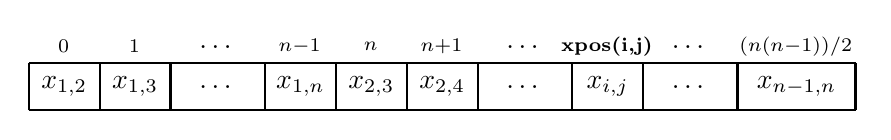
\begin{tikzpicture}[thick,scale=0.6]
			\draw (0,0) -- (17.5,0);
			\draw (0,1) -- (17.5,1);
			\foreach \p [count=\i from 0] in {0,1.5,3,5,6.5,8,9.5,11.5,13,15,17.5} {
				\draw (\p,0) -- (\p,1);
			}
			\path (.5,.5) (0.75,1.35) node{$_{0}$} ++(1.5,0) node{$_{1}$} ++(1.75,0) node{$\dots$} ++(1.75,0) 
									node{$_{n-1}$} ++(1.5,0) node{$_{n}$} ++(1.5,0) node{$_{n+1}$} ++(1.75,0) node{$\dots$} ++(1.75,0)
									node{$_{\textbf{xpos(i,j)}}$} ++(1.75,0) node{$\dots$} ++(2.25,0)
									node{$_{(n(n - 1)) / 2}$};
			\path (.5,.5) (0.75,0.5) node{$x_{1,2}$} ++(1.5,0) node{$x_{1,3}$} ++(1.75,0) node{$\dots$} ++(1.75,0) 
									node{$x_{1,n}$} ++(1.5,0) node{$x_{2,3}$} ++(1.5,0) node{$x_{2,4}$} ++(1.75,0) node{$\dots$} ++(1.75,0)
									node{$x_{i,j}$} ++(1.75,0) node{$\dots$} ++(2.25,0)
									node{$x_{n-1,n}$};
		\end{tikzpicture}
	\end{center}
	\caption{CPLEX solution array} \label{fig:CPLEXxstar}
\end{figure}

Given such an array, it can be quite troublesome to find an edge given its connected nodes $(i,j)$.
To extract the position of edge $(i,j)$ one must use a function like the \textbf{xpos} function, as shown in \figurename{ \ref{fig:xpos}}.

\begin{figure}[htbp]
	\begin{function}[H]
		\TitleOfAlgo{\textbf{xpos}}
		\SetKwInOut{Input}{input}
		\SetKwInOut{Output}{output}
		\Input{$i$, $j$, $|V|$}
		\Output{position of $edge(i,j)$ in CPLEX notation}
		\vspace{2mm}
		\If{$i = j$}{ Error\; }
		\If{$i > j$}{ $i \Leftrightarrow j$\; }
		\Return{$i |V| + j - \frac{(i + 1) (i + 2)}{2}$}
	\end{function}
	\caption{Pseudocode of the xpos function, used to extract the position of an edge $(i,j)$ in a CPLEX solution array}\label{fig:xpos}
\end{figure}

Saving the solution this way requires a lot of space as well as an increase in indexing complexity caused by the need use the \textbf{xpos} function.
Therefore, as soon as CPLEX is done, it's more efficient to convert the solution into a more specialized format.
The data structure used to store the solution in the previous chapters is not as straightforward to use.
This is because the output of CPLEX, as described in the following chapters, might contain two or more subtours.
Unfortunately, the solution format used until now cannot efficiently handle solutions containing subtours, necessitating the introduction of a different format.
The Successors format enables efficient storage of subtours without requiring additional structures or the use of the \textbf{xpos} function.
The format consists of an array of size $|V|$, where each position $i$ contains the index of the successor of node $i$ itself.
%A comparison between all solution formats used in this project is illustrated in \figurename{ \ref{fig:cpxsuccEx}}.

\begin{figure}[htbp]
	\begin{center}
		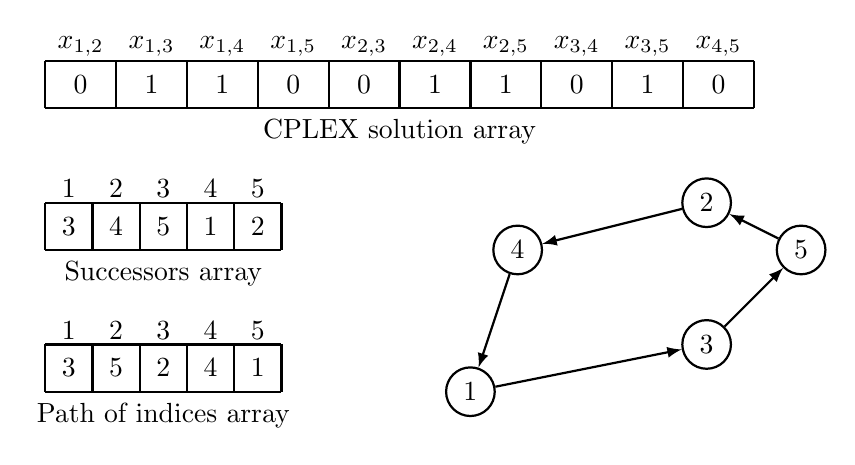
\begin{tikzpicture}[thick,scale=.6]
			% CPLEX ARRAY
			\path (.5,.5) (0.75,8.3) node{$x_{1,2}$} ++(1.5,0) node{$x_{1,3}$} ++(1.5,0) node{$x_{1,4}$} ++(1.5,0) node{$x_{1,5}$} ++(1.5,0)
									 node{$x_{2,3}$} ++(1.5,0) node{$x_{2,4}$} ++(1.5,0) node{$x_{2,5}$} ++(1.5,0) 
									 node{$x_{3,4}$} ++(1.5,0) node{$x_{3,5}$} ++(1.5,0)
									 node{$x_{4,5}$} ++(1.5,0);
			\path (.5,.5) (0.75,7.5) node{$0$} ++(1.5,0) node{$1$} ++(1.5,0) node{$1$} ++(1.5,0) node{$0$} ++(1.5,0)
									 node{$0$} ++(1.5,0) node{$1$} ++(1.5,0) node{$1$} ++(1.5,0) 
									 node{$0$} ++(1.5,0) node{$1$} ++(1.5,0)
									 node{$0$} ++(1.5,0);
			\draw (0,7) -- (15,7);
			\draw (0,8) -- (15,8);
			\foreach \p [count=\i from 0] in {0,1.5,3,4.5,6,7.5,9,10.5,12,13.5,15} {
				\draw (\p,7) -- (\p,8);
			}
			\draw (7.5,6.5) node{CPLEX solution array};
			
			% SUCCESSORS ARRAY
			\draw (0,4) grid (5,5);
			\draw (2.5,3.5) node{Successors array};
			\path (.5,.5) (0.5,5.3) node{$1$} ++(1,0) node{$2$} ++(1,0) node{$3$} ++(1,0) node{$4$} ++(1,0) node{$5$};
			\path (.5,.5) (0.5,4.5) node{$3$} ++(1,0) node{$4$} ++(1,0) node{$5$} ++(1,0) node{$1$} ++(1,0) node{$2$};

			% INDEXPATH ARRAY
			\draw (0,1) grid (5,2);
			\draw (2.5,0.5) node{Path of indices array};
			\path (.5,.5) (0.5,2.3) node{$1$} ++(1,0) node{$2$} ++(1,0) node{$3$} ++(1,0) node{$4$} ++(1,0) node{$5$};
			\path (.5,.5) (0.5,1.5) node{$3$} ++(1,0) node{$5$} ++(1,0) node{$2$} ++(1,0) node{$4$} ++(1,0) node{$1$};


			\node[circle, draw, fill=white] (A) at (9,1) {1};
	        \node[circle, draw, fill=white] (B) at (14,5) {2};
	        \node[circle, draw, fill=white] (C) at (14,2) {3};
			\node[circle, draw, fill=white] (D) at (10,4) {4};
	        \node[circle, draw, fill=white] (E) at (16,4) {5};

			\draw [-latex] (A) -- (C);
			\draw [-latex] (C) -- (E);
			\draw [-latex] (E) -- (B);
			\draw [-latex] (B) -- (D);
			\draw [-latex] (D) -- (A);
		\end{tikzpicture}
	\end{center}
	\caption{Cplex and Successors solution notations} \label{fig:cpxsuccEx}
\end{figure}


\chapter{Exact Solvers}

%We call Exact Solvers those algorithms that allow us to solve the TSP to optimality, namely the Benders method and the famous Branch and Cut method. They are both based on the ILP model described before, both start without any SEC, but they add them as they SEC are violated and both use CPLEX, although in different ways.
We refer to Exact Solvers as algorithms that enable us to solve the TSP optimally.
Specifically, two well-known methods fall into this category: the Benders method and the renowned Branch and Cut method.
Both of these approaches are based around CPLEX.

\section{Benders}

Benders is a method that, given enough time, allows to find an optimal solution to the TSP.
The algorithm consists in running CPLEX's ILP solver multiple times on the problem $p$ obtained using CPLEX Initialization (\figurename{ \ref{fig:CPLEXinit}}).
This is done until the solution $x^*$ obtained at the current iteration does not contain any subtours, or the number of subtours in the solution is equal to one.
Every time $x^*$ contains two or more subtours $x^*$ must be rejected and a number equal to the number of subtours found of SEC must be added to $p$.
This means that every iteration two or more SEC are added or the $x^*$ is optimal.
The basic version of the Benders algorithm is described in \figurename{ \ref{fig:CPLEXinit}}.

\begin{figure}[htbp]
	\textbf{Benders} \\
	\begin{algorithm}[H]
		\SetKwInOut{Input}{input}
		\SetKwInOut{Output}{output}
		\Input{Graph $G(V,E)$ fully connected }
		\Output{Optimal Solution $x^*$}
		\vspace{2mm}
		$p \gets$ CPLEX Initialization (\ref{fig:CPLEXinit})\\
		\While{$true$}{
			$x^* \gets$ optimal solution of $p$\\
			$count \gets$ number of subtours in $X^*$\\
			\uIf{$count = 1$}{
				$x^*$ is valid \\
				break \\
			}
			\uElse{
				\ForEach{subtour $s \in x^*$}{ 
					add SEC violated by $s$ to $p$ \\
				}
			}
		}
		\Return{$x^*$}
	\end{algorithm}
	\caption{Basic version of Benders algorithm} \label{fig:benders}
\end{figure}

\subsection{Warm Start}

Warm starting is a procedure that involves supplying the solver with an initial feasible solution or a partial solution.
This solution can originate from heuristic methods, results from previous optimization runs, or domain-specific insights.
The initial solution serves as a valuable starting point for the optimization algorithm, profoundly influencing the search process in several key ways.
In the branch and bound algorithm the solver systematically explores branches of a decision tree that represent subsets of feasible solutions.
By integrating a warm start, the solver benefits in multiple aspects. Firstly, the initial feasible solution provides a concrete starting point, which the solver can immediately use to initialize the search.
This starting point offers an initial upper bound for minimization problems, thus narrowing the search space from the outset and allowing more effective pruning of non-promising branches.
In terms of node selection and pruning, the initial feasible solution enables the solver to prioritize nodes within the decision tree that are more likely to yield optimal or near-optimal solutions.
This prioritization is based on the initial bounds provided by the warm start solution.
Consequently, the solver can prune the decision tree more aggressively; if a node's bound is worse than the initial bound provided by the warm start solution, that node and its descendants can be discarded, reducing the computational effort required.
Furthermore, the initial feasible solution guides the solver's search towards more promising regions of the solution space, leading to faster convergence.
The warm start also aids in tightening the dual bounds, narrowing the optimality gap, and expediting the overall optimization process.
In Benders's case, as well as all other algorithms that use CPLEX in this project, a warm start consists in a solution obtained using an algorithm like ones from the previous chapters or a combination of them.
The time limit also includes the time necessary to find the warm starting solution and corresponds to 5\% of the whole


\subsection{Patching Heuristic}

It's certain that Benders will eventually find the optimal solution of all TSP instances used in this project, however, depending on the size of the instance, getting to such solution can take a lot of time.
As an example, on almost all of the instances with 100 nodes, Benders takes less than a second to reach optimality, however as the number of nodes rises close to 500 the time it needs goes past 100 seconds.
This means that when Benders is required to run within a specific time limit it may end up running out of time without producing any valid solution.
To address this issue it is possible to use the solutions produced at each step iteration of Benders.
Those solutions contain at least two subtours, hence, they are not valid solution for the TSP, however they can be "patched" by merging the subtours into one.
Patching Heuristic is a greedy heuristic algorithm that merges all subtours contained in a solution into one, generating a valid solution, as shown by the pseudocode in \figurename{ \ref{fig:patchHeur}}.
The basic reasoning behind it is to find merge two subtours at each iteration until only one subtour remain.
Patching Heuristic begins by identifying two subtours to be merged.
In each iteration, select an edge from each subtour to be removed.
These edges are chosen such that their removal creates openings at the endpoints of the subtours.
For example, consider subtours AA and BB with edges $(a_i,a_{i+1})$ in $A$ and $(b_j,b_{j+1})$ in BB.
Remove these edges to create the openings $(a_i \leftarrow a_{i+1})$ and $(b_j \leftarrow b_{j+1})$.
Next, introduce new edges to bridge these openings. Specifically, connect node $a_i$ to node $b_j$ and node $a_{i+1}$ to node $b_{j+1}$.
This effectively merges the two subtours by forming a larger tour that includes all nodes from both subtours while maintaining the constraints of the TSP.
Continue this process iteratively, selecting pairs of subtours and merging them in a similar fashion until only one tour remains.
The choice of which subtours to merge and which edges to be used in the merge is done by simulating all possibile merges between all couples of subtours and combinations of edges and selecting the merge that increases the objective value the least.
The algorithm ensures that at each step, the total number of subtours decreases, ultimately resulting in a single subtour that spans all nodes in the graph.
The final outcome is a feasible TSP solution where a single tour visits each node exactly once and returns to the starting node.

\begin{figure}[htbp]
	\begin{center}
		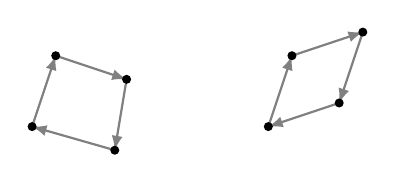
\begin{tikzpicture}[thick,scale=.6]

			\draw [-latex, gray] (1,0.5) -- (1.5,2);
			\draw [-latex, gray] (1.5,2) -- (3,1.5);
			\draw [-latex, gray] (3,1.5) -- (2.75,0);
			\draw [-latex, gray] (2.75,0) -- (1,0.5);
			
			\draw [-latex, gray] (6,0.5) -- (6.5,2);
			\draw [-latex, gray] (6.5,2) -- (8,2.5);
			\draw [-latex, gray] (8,2.5) -- (7.5,1);
			\draw [-latex, gray] (7.5,1) -- (6,0.5);
			

			\foreach \p [count=\i] in {(1,0.5), (1.5,2), (3,1.5), (2.75,0)} {
				\filldraw [black] \p circle (2pt);
			}

			\foreach \p [count=\i] in {(6,0.5), (6.5,2), (8,2.5), (7.5,1)} {
				\filldraw [black] \p circle (2pt);
			}
		\end{tikzpicture}
		\\
		$\Downarrow$
		\\
		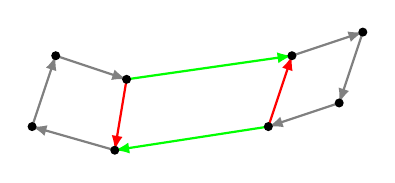
\begin{tikzpicture}[thick,scale=.6]

			\draw [-latex, gray] (1,0.5) -- (1.5,2);
			\draw [-latex, gray] (1.5,2) -- (3,1.5);
			\draw [-latex, red] (3,1.5) -- (2.75,0);
			\draw [-latex, gray] (2.75,0) -- (1,0.5);
			
			\draw [-latex, red] (6,0.5) -- (6.5,2);
			\draw [-latex, gray] (6.5,2) -- (8,2.5);
			\draw [-latex, gray] (8,2.5) -- (7.5,1);
			\draw [-latex, gray] (7.5,1) -- (6,0.5);

			\draw [-latex, green] (3,1.5) -- (6.5,2);
			\draw [-latex, green] (6,0.5) -- (2.75,0);
			

			\foreach \p [count=\i] in {(1,0.5), (1.5,2), (3,1.5), (2.75,0)} {
				\filldraw [black] \p circle (2pt);
			}

			\foreach \p [count=\i] in {(6,0.5), (6.5,2), (8,2.5), (7.5,1)} {
				\filldraw [black] \p circle (2pt);
			}
		\end{tikzpicture}
		\\
		$\Downarrow$
		\\
		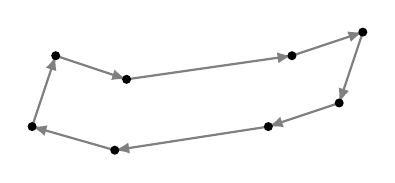
\begin{tikzpicture}[thick,scale=.6]

			\draw [-latex, gray] (1,0.5) -- (1.5,2);
			\draw [-latex, gray] (1.5,2) -- (3,1.5);
			% \draw [-latex, red] (3,1.5) -- (2.75,0);
			\draw [-latex, gray] (2.75,0) -- (1,0.5);
			
			% \draw [-latex, red] (6,0.5) -- (6.5,2);
			\draw [-latex, gray] (6.5,2) -- (8,2.5);
			\draw [-latex, gray] (8,2.5) -- (7.5,1);
			\draw [-latex, gray] (7.5,1) -- (6,0.5);

			\draw [-latex, gray] (3,1.5) -- (6.5,2);
			\draw [-latex, gray] (6,0.5) -- (2.75,0);
			

			\foreach \p [count=\i] in {(1,0.5), (1.5,2), (3,1.5), (2.75,0)} {
				\filldraw [black] \p circle (2pt);
				% \draw \p+(0,0.5) node {\i};	
			}

			\foreach \p [count=\i] in {(6,0.5), (6.5,2), (8,2.5), (7.5,1)} {
				\filldraw [black] \p circle (2pt);
				% \draw \p+(0,0.5) node {\i};	
			}
		\end{tikzpicture}
	\end{center}
	\caption{Example of merging two subtours} \label{fig:examplePatching}
\end{figure}

\begin{figure}[htbp]
	\textbf{Patching Heuristic} \\
	\begin{algorithm}[H]
		\SetKwInOut{Input}{input}
		\SetKwInOut{Output}{output}
		\Input{
			Graph $G(V,E)$ fully connected \newline
			$c_{ij}=$ cost of $edge(i,j) \in |E|$ $\forall$ $i,j \in V$ with $i \neq j$ \newline
			$S$ solution containing two or more subtours
			}
		\Output{Valid solution $S$}
		\vspace{2mm}
		$count \gets$ number of subtours in $S$ \\
		\While{$count > 1$ }{
			$e_{i,j} \in s_1$, $e_{k,l} \in s_2$ $\gets$ Find Best Patching Edges \\%(procedure similar to 2opt) \\
			merge $s_1$ with $s_2$ by swapping $e_{i,j}$, $e_{k,l}$ with $e_{i,l}$, $e_{k,j}$ (or with $e_{i,k}$, $e_{j,l}$ if it is cheaper on the cost) \\
			$count \gets count - 1$ 
		}
		\Return{$S$}
	\end{algorithm}
	\caption{Patching Heuristic pseudocode} \label{fig:patchHeur}
\end{figure}

With this method the chance of Benders of not producing any solution is greatly reduced, but not nullified since CPLEX needs to finish at least once.
Patching Heuristic allows to generate a new solution at each iteration of Benders and, as the number of SEC added increases the quality of such solution usually increases.
This happens because the solution that is produced resembles more and more an optimal solution as Benders iterates, sometimes it even happens that an optimal solution is found by patching subtours before the end of Benders, however the only way to verify optimality is to wait for the algorithm to finish.
Furthermore this technique can be applied together with warm starting: by keeping the best solution obtained, at each iteration such solution can be used to warm start cplex.
Since better solutions than the first warm starting solution are likely to be produced at some point, efficiency of subtree pruning will also increase as the best solution quality improves, resulting, theoretically, in better efficiency.

\subsection{Efficiency}
Benders, being an exact algorithm, automatically stops once it finds the optimal solution and the runtime changes at every run in a random way, depending on the random seed of CPLEX. 
This means that it's more interesting to study time efficiency than the performance given by the cost of the resulting solution.
Since the algorithm is quite slow the instances on which it has run are all below 1000 nodes\footnote{Instances ts225 and p654 were excluded since for some reason the solving time on those is way higher compared to the others. Such difference would offset too much time limits hence they were removed}, with an increased time limit compared to previous testing which allowed to always reach optimality.
Specifying the time limit is mandatory since some of the tests use warm start which requires a global time limit to obtain it's own time limit that is set to either 5\% or 1\%.
% \tablename{ \ref{tab:bendersSimple}} contains the average runtime of Benders of five runs on each instance with different seeds, however it must be noted that time used to find the warm starting solution is not included.
The time limits used to gather data as set according to \tablename{ \ref{tab:bendersTlims}}.

\begin{table}[h]
	\centering
	\caption{Time limits used to run benders while gathering data} \label{tab:bendersTlims}	\vspace{2mm}
	\begin{tabular}{|C{22mm}|C{21mm}|C{28mm}|C{28mm}|}
		\hline \multirow{2}{22mm}{\textbf{Nodes range}} & \multicolumn{3}{c|}{\textbf{Time Limits}} \\ 
		\cline{2-4} & \textbf{Global} & \textbf{Warm Start 5\%} & \textbf{Warm Start 1\%} \\
		\hline
		0 - 80 & 5 seconds & 0.25 seconds & 0.05 seconds\\
		100 - 200 & 30 seconds & 1.5 seconds & 0.3 seconds\\
		220 - 320 & 120 seconds & 6 seconds & 1.2 seconds\\
		400 - 500 & 300 seconds & 15 seconds & 3 seconds\\
		500 - 800 & 400 seconds & 20 seconds & 4 seconds\\
		\hline
	\end{tabular}
\end{table} 
 
% \vspace{5mm}
% \begin{longtable}{L{15mm}C{15mm}C{22mm}C{18mm}C{22mm}}
% 	\caption{Benders only runtimes in seconds (with 1\% time limit on warm start)} \label{tab:bendersSimple}\\
% 	\endfirsthead
% 	\textbf{Instance} & \textbf{Basic} & \textbf{Warm Start} & \textbf{Patching} & \textbf{Warm Start + Patching}
% 	\endhead
% 	\textbf{Instance} & \textbf{Basic} & \textbf{Warm Start} & \textbf{Patching} & \textbf{Warm Start + Patching}
% 	\csvreader[head to column names]{csv/benders_simple-runtime.csv}{}% use head of csv as column names
% 	{\\ \csvcoli & \csvcolii & \csvcoliii & \csvcoliv & \csvcolv}% specify your coloumns here
% 	\\
% \end{longtable}

\begin{figure}[htbp]
	\centering 
	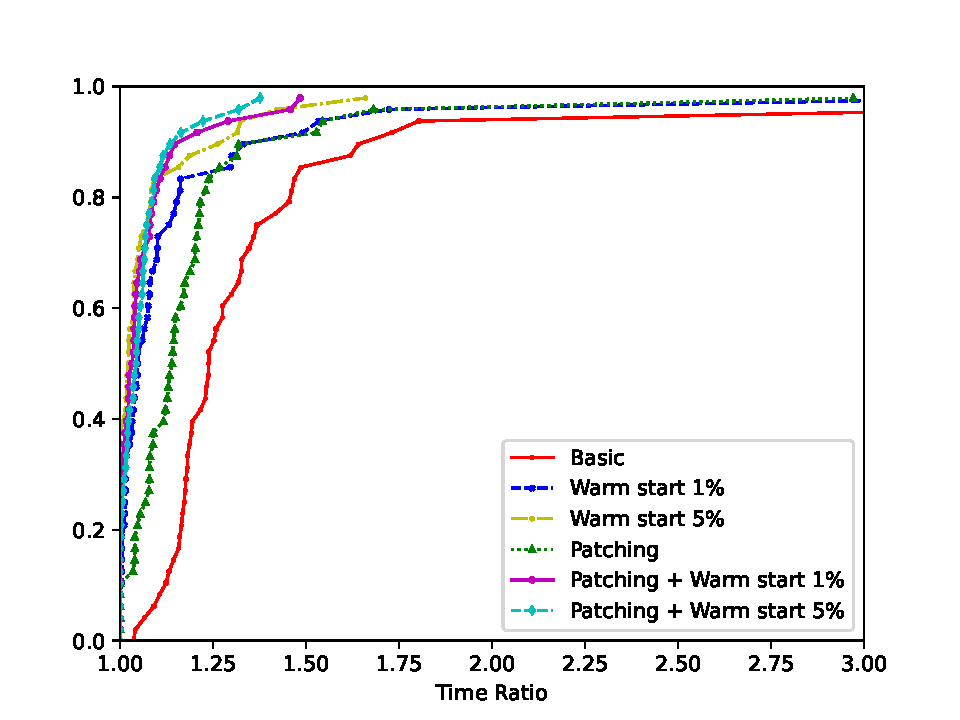
\includegraphics[scale=0.73]{benders_simple.pdf}
	\caption{Performance profile graph on runtimes of benders \label{fig:bendersSimplePerfProf}}
\end{figure}

To obtain a more insightful comparison \figurename{ \ref{fig:bendersSimplePerfProf}} compares all average runtimes collected exluding warm start time.
The basic version of Benders falls short of the ones that use patching and warm start basically every time, while it's clear that using any kind of warm starting, including its combination with Patching, improves efficiency by a noticeable amount.
Starting Benders usign an already existing solution seems to also have an improving effect, with the better solution, that is intuitevly found by spending more time on its computation, yielding an improvement very small that could very well be considered within standard deviation of tests when Patching is applied as well.
However the time taken to find that first solution must also be taken into account.

\begin{figure}[htbp]
	\centering
	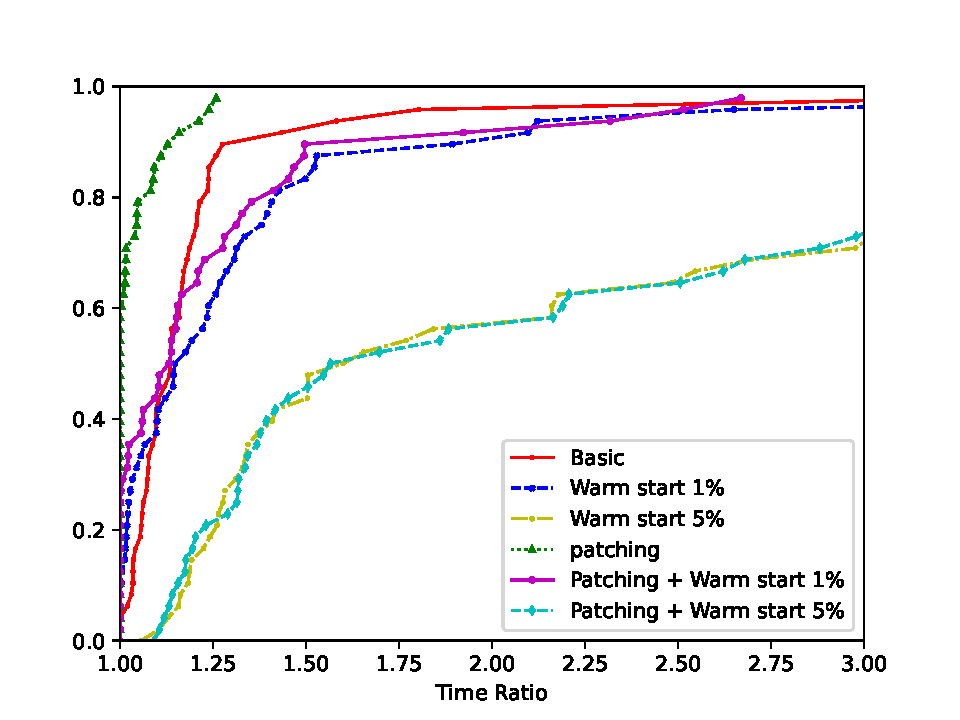
\includegraphics[scale=0.73]{benders_full.pdf}
	\caption{Performance profile graph on runtimes of benders including warm start time \label{fig:bendersFullPerfProf}}
\end{figure}

In \figurename{ \ref{fig:bendersFullPerfProf}} it's clear to see that the time needed to get the first solution using external means than Benders is actually greatly affecting the efficiency of the run in a negative way.
The efficiency decreases so much that even the basic version of Benders is on par or better, while the best for overall runtime is given by only Patching.
It's also possible to advance the hypothesis that the first solution doesn't need to be a strictly good one when Patching is involved, since Patching will find a better solutions during the execution, it would be beneficial to define a specific way to find the first solution in order to waste least possible amount of time on it.
Further testing may be considered to be done on top of such hypothesis by using even less time to find the first warm starting solution, that however is outside of the scope of this project.

% \newpage

\section{Branch and Cut}
Branch and Cut is a method that builds upon the Branch and Bound technique and improves it using knowledge specific on the problem domain to find more efficient cuts.
The simplest way to implement this algorithm is to check for subtours and add necessary SEC directly within \textit{CPXmipopt}.
To achieve this CPLEX allows the user to define some code that will be called while CPLEX solver itself is running, thus allowing to add SEC before \textit{CPXmipopt} terminates losing the cut pool and other useful informations.
The generic callback technique allows to run user codes at specified points in the execution, like when a candidate solution is found or when the LP relaxation is solved.
For the most simple implementation of Branch and Cut the callback code is just needed to run upon discovering a solution candidate so such solution can be checked for subtours and SEC can be added to the cut pool.

\begin{figure}[htbp]
	\textbf{Basic Candidate Callback} \\
	\begin{algorithm}[H]
		\SetKwInOut{Input}{input}
		\Input{ 
			CPLEX problem $p$ \newline
			candidate solution $x$ \newline
			best solution found until now $b$
		}
		\vspace{2mm}
		$t \gets$ convert $x$ to successors solution\\
		\uIf{number of subtours in $t$ $>$ 1}{
			\ForEach{subtour $s \in t$}{ 
				add SEC violated by $s$ to $p$ \\
			}
			reject candidate $x$ \\
		}
		\uElseIf{cost($t$) $<$ cost($b$) }{$b \gets t$}
	\end{algorithm}
	\caption{Basic Callback function} \label{fig:callbackBase}
\end{figure}
\begin{figure}[htbp]
	\textbf{Branch and Cut} \\
	\begin{algorithm}[H]
		\SetKwInOut{Input}{input}
		\SetKwInOut{Output}{output}
		\Input{Graph $G(V,E)$ fully connected }
		\Output{Optimal Solution $x^*$}
		\vspace{2mm}
		$p \gets$ CPLEX Initialization (\ref{fig:CPLEXinit})\\
		set CPLEX callback function \textbf{Candidate Callback}\\
		$x^* \gets$ optimal solution of $p$\\
		\Return{$x^*$}
	\end{algorithm}
	\caption{Branch and Cut algorithm} \label{fig:branchAndCut}
\end{figure}

The Branch and Cut algorithm implemented this way still has the same weakness of Benders: it's not sure that a feasible solution will be produced until the optimal solution is found.
The problem is solved the same way as Benders's, it's simply necessary to run Patching Heuristic and every time a candidate is found a feasible solution will be produced as well.
With the same reasoning the warm start procedure can also be applied.

\subsection{Posting}
During the execution of Branch and Cut it's possible for a solution better than the ones observed before it to apper while navigating the search tree.
Solutions obtained this way cannot be used to warm start CPLEX because in this Branch and Cut implementation there is only one chance for a warm start, that is at the very beginning since \textit{CPXmipopt} runs only once.
To allow CPLEX to reap similar benefits of the warm start and Patching of Benders while the solver is running a similar but callback-specific operation called Posting needs to be performed.
The Posting procedure allows the user to give CPLEX a feasible solution during the solving procedure to improve the pruning of the search tree yielding overall better time efficiency.
A feasible solution to use in the Posting procedure can be either found as candidate while exploring the search tree or by patching an invalid candidate solution.
Posting can be viewed as a low level implementation of the warm start technique as the advantages given by both methods are indeed very similar.
With the implementation of the solution posting the candidate callback is complete and it's shown in \figurename{ \ref{fig:callbackComplete}}

\begin{figure}[htbp]
	\textbf{Complete Candidate Callback} \\
	\begin{algorithm}[H]
		\SetKwInOut{Input}{input}
		\Input{ 
			CPLEX problem $p$ \newline
			candidate solution $x$ \newline
			best solution found until now $b$
		}
		\vspace{2mm}
		$t \gets$ convert $x$ to successors solution\\
		\uIf{number of subtours in $t$ $>$ 1}{
			\ForEach{subtour $s \in t$}{ 
				add SEC violated by $s$ to $p$ \\
			}
			reject candidate $x$ \\
			$t \gets$ \textbf{Patching Heuristic}($t$) (\ref{fig:patchHeur})
		}
		\tcc{$t$ is certainly a valid solution at point}
		\uIf{cost($t$) $<$ cost($b$) }{
			$b \gets t$\\
			\textbf{Post Solution} $t$
		}
	\end{algorithm}
	\caption{Candidate callback implementing both patching and posting} \label{fig:callbackComplete}
\end{figure}

\subsection{Concorde and  Usercuts}

The Concorde TSP Solver, developed by William Cook and his collaborators, is one of the most advanced and effective tools for solving large-scale instances of the TSP.
Using it as a C library, Concorde provides with multiple useful functions including those that allow to compute advanced cuts on a fractional solution in Branch and Cut.
These cuts come in the form simple Gomory cuts as well as TSP specific cuts, which allow to add SEC in advance, avoiding spending time to reach some invalid candidate solutions, although not avoiding them entirely.
A brief description on how these specific cuts are found is described below.
Initially, the LP relaxation of the TSP is solved, where the integer constraints on the decision variables \( x_{ij} \) are relaxed, allowing them to take fractional values between 0 and 1.
The resultant solution provides fractional edge values \( x_{ij}^* \), representing the degree to which each edge \( (i,j) \) is included in the tour.
Using the fractional solution, a residual graph \( G = (V, E) \) is constructed.
In this graph, nodes \( V \) correspond to cities, and edges \( E \) are weighted by the fractional values \( x_{ij}^* \), which serve as the capacities of the edges.
To identify violated subtour elimination constraints, a maximum flow algorithm is employed.
By selecting a source node \( s \) and a sink node \( t \) from the graph, the maximum flow from \( s \) to \( t \) is computed.
The maximum flow value corresponds to the minimum capacity cut that separates \( s \) from \( t \).
The min cut found after computing the max flow separates the graph into two disjoint subsets \( S \) and \( T \).
The sum of the capacities of the edges crossing from \( S \) to \( T \) is minimized.
If the sum of the fractional values \( x_{ij}^* \) across the cut is less than \( |S| - 1 \), it indicates that this cut violates the subtour elimination constraint, implying the existence of a subtour that does not connect all nodes in a single tour.
Upon identifying a violated subtour elimination constraint, it is added to the LP formulation and the procedure then continues.

In order for the procedure above to work it needs to get as input the solution at the LP relaxation point, thus requiring to complicate a bit the callback function.
In fact before it was said that the callback was only executed on discovering a new candidate solution which is an integer solution.
To obtain access to the relaxation solution it is necessary to let CPLEX invoke the callback at both candidate and relaxation point, dividing the callback into two parts.
That said the candidate callback remains the same while the relaxation callback, \figurename{ \ref{fig:relaxCallback}}, is the one which implements usercuts.

\begin{figure}[htbp]
	\textbf{Relaxation Callback} \\
	\begin{algorithm}[H]
		\SetKwInOut{Input}{input}
		\Input{ 
			CPLEX problem $p$ \newline
			relaxation optimal solution $x$ \newline
		}
		\vspace{2mm}
		$comps \gets$ \textbf{CCcut\_connect\_components}($x$) \\
		\uIf{number of components in $comps$ $>$ 1}{
			\tcp{If multiple components are detected add cuts to invalidate them}
			\ForEach{component $c \in comps$}{ 
				add SEC violated by $c$ to $p$ as usercut\\
			}
		}
		\uElseIf{number of components in $comps$ $=$ 1}{
			\tcp{If only one component is detected use Concorde to find the best cut/cuts}
			$cuts \gets$ \textbf{CCcut\_violated\_cuts}($x$)\\
			\ForEach{cut $c \in cuts$}{ 
				add cut by $c$ to $p$ as usercut\\
			}
		}
	\end{algorithm}
	\caption{Relaxation Callback implementing usercuts using Concorde library} \label{fig:relaxCallback}
\end{figure}

\subsection{Efficiency}
For the same reason explained with Benders, this section will discuss the effectiveness of each of the strategies described above using the execution time as the main metric.
\begin{figure}[htbp]
	\centering
	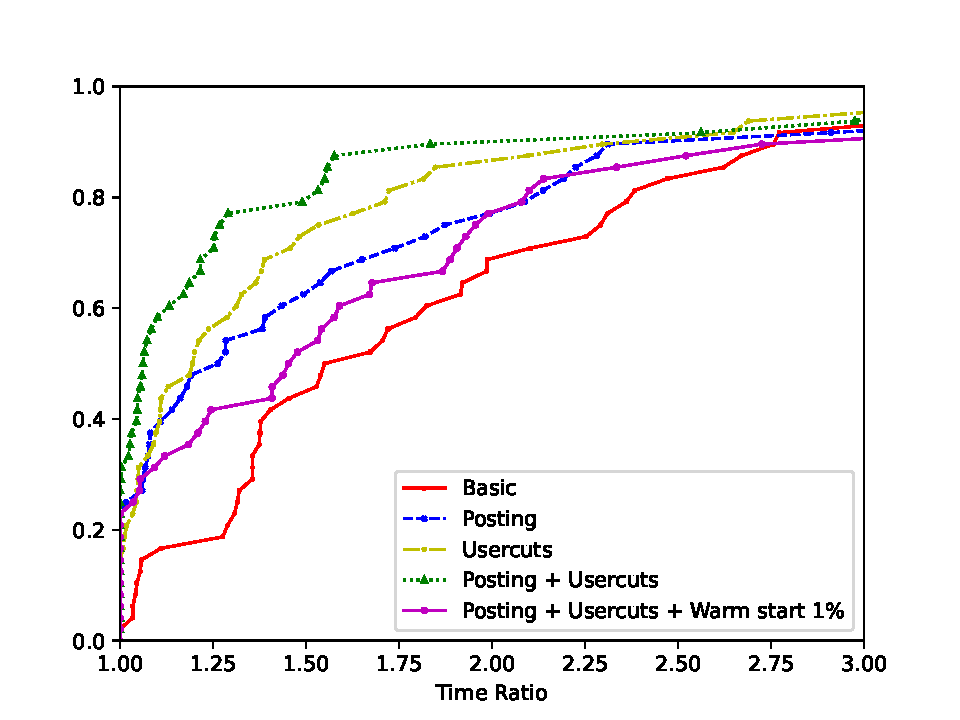
\includegraphics[scale=0.73]{branch-cut_full_MOD.pdf}
	\caption{Performance profile graph on the execution time of the whole program using Branch and Cut algorithm \label{fig:branchCutFull}}
\end{figure}
By inspecting \figurename{ \ref{fig:branchCutFull}} it's possible to see that the best possible configuration of the Branch and Cut method is a cobination of both Posting and Usercuts, with what it seems to be a more impactful improvement given by the latter.
Posting alone is still able to outperform the basic version of the algorithm, while using warm start is not the worst combination, managing to perform slightly worse than Posting.
The tables turn completely when not taking into consideration the warm start time.
\begin{figure}[htbp]
	\centering
	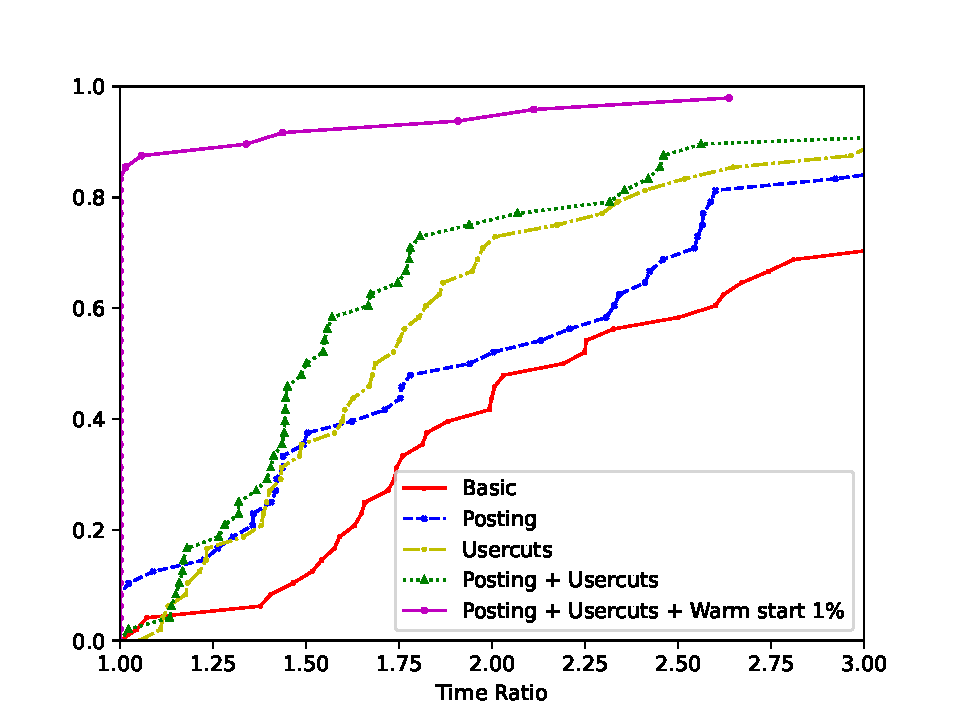
\includegraphics[scale=0.73]{branch-cut_simple_MOD.pdf}
	\caption{Performance profile graph on the execution time of the Branch and Cut algorithm (excluding warm start time) \label{fig:branchCutSimple}}
\end{figure}
As \figurename{ \ref{fig:branchCutSimple}} clearly shows, the time took by Branch and Cut to solve an instance using the warm start technique in combination with both Posting and Usercuts, is undoubtely the best.
Such a result is very similar to Benders's case of warm starting, where the efficiency using warm start would be hindered by the first solution time.
This situation gives more gravity to a matter secondary to the algorithm itself: what is the exact time needed obtain a good enough solution to use as warm start while not deteriorating the algorithm efficiency as a whole?
An interesting experiment would be to run again all tests while instead of optimizing the warm start solution according to a time limit, obtain the first possible solution and optimizing it according to a number of iterations.
As an example the first solution could be obtained by running Nearest Neightbor $k$ times with $k=10$ or some other reasonably low value and than optimize the best solution obtained using 2-Opt.
Since such kind of experiment would require major changes to the project code it was deemed outside the scope of the project. 

\section{Comparison}	
Finally \figurename{ \ref{fig:bendersBranchCut}} directly compares Benders method and Branch and Cut algorithm, both with and without using the warm starting technique.
On average Branch and Cut runs three times faster compared to Benders, however, in some instances, the latter still outperforms the first.

\begin{figure}[htbp]
	\centering
	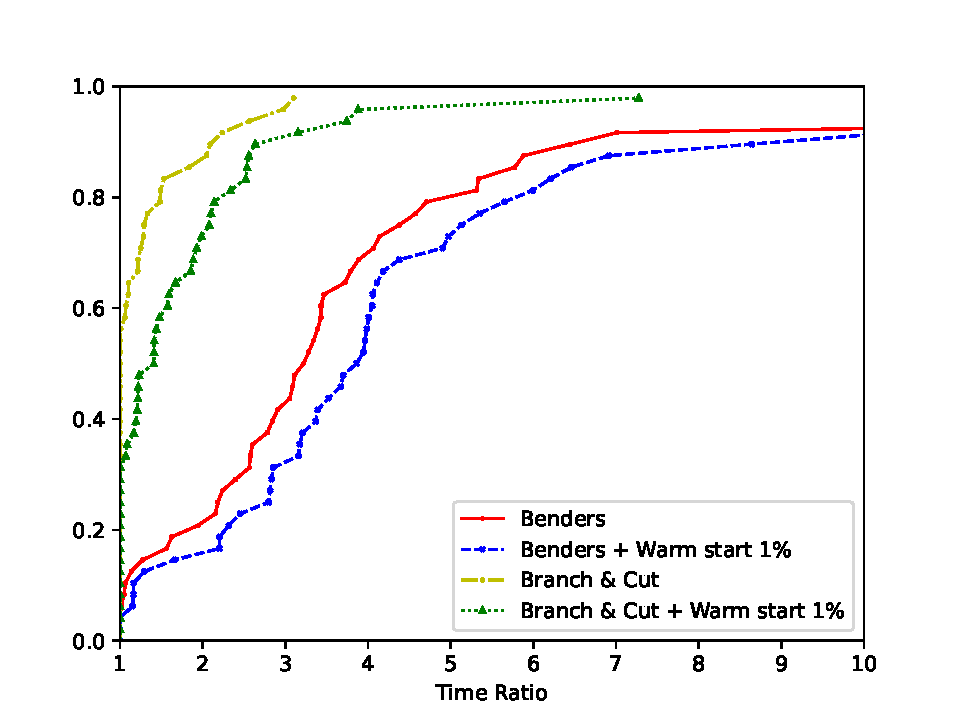
\includegraphics[scale=0.73]{benders-branch-cut.pdf}
	\caption{Comparison between Benders and Branch and Cut\label{fig:bendersBranchCut}}
\end{figure}

\chapter{Matheuristics}
Matheuristics, a fusion of mathematical programming and metaheuristic techniques, have emerged as robust and versatile approaches for solving complex optimization problems.
These hybrid methods leverage the strengths of both mathematical programming, which provides exact and rigorous solutions, and metaheuristics, which offer flexibility and the ability to escape local optima.
By integrating these two paradigms, matheuristics aim to efficiently solve large-scale and complex problems that are otherwise intractable using conventional methods alone.
This chapter will address two Matheuristics, \textbf{Hard Fixing} and \textbf{Local Branching}, which rely on the use of CPLEX to optimize an already existing solution.

\section{Hard Fixing}
Hard Fixing is a Matheuristic that optimize an already feasible TSP solution "fixing" in place some of the edges of the solution and optimizing the rest using CPLEX.
This procedure begins with the generation of an initial feasible solution, typically derived from a heuristic or metaheuristic method such as Tabu Search or VNS.
Once an initial solution is obtained, the process of "hard fixing" commences.
In this context, hard fixing refers to selecting a subset of the solution's components and fixing them in place with the goal of reducing the problem size and complexity for subsequent optimization steps.

There are multiple ways to choose which edges to fix and which edges to keep "free":

\begin{itemize}
    \item \textbf{Random Fix}\\
    The easiest method to implement is to fix edges in the solution at random up to a certain threshold.
    As far as effectivenss goes, this method relies mostly on luck since it's a completely random method the change of locking a set of edges that allows a good optimization can be selected purely by chance.
    \begin{figure}[H]
        \centering
        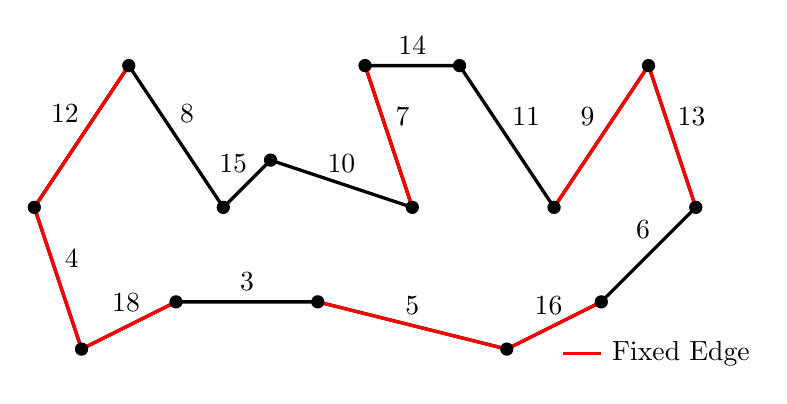
\begin{tikzpicture}[thick,scale=.6]
            \coordinate (A) at (0, 0);\coordinate (B) at (2, 3);\coordinate (C) at (4, 0);\coordinate (D) at (1, -3);\coordinate (E) at (3, -2);\coordinate (F) at (5, 1);\coordinate (G) at (6, -2);\coordinate (H) at (8, 0);\coordinate (I) at (7, 3);\coordinate (J) at (9, 3);\coordinate (K) at (11, 0);\coordinate (L) at (10, -3);\coordinate (M) at (12, -2);\coordinate (N) at (14, 0);\coordinate (O) at (13, 3);

            \draw[-,very thick] (A) -- node[above,yshift=1,xshift=-6] {12} (B) -- node[above,yshift=1,xshift=4] {8} (C) --node[above,xshift=-5] {15} (F) -- node[above] {10} (H) -- node[above,xshift=5] {7} (I) -- node[above] {14} (J) -- node[above,xshift=7] {11} (K) -- node[above,xshift=-5] {9} (O) -- node[above,xshift=7] {13} (N) -- node[above,yshift=2,xshift=-2] {6} (M) -- node[above,xshift=-2] {16} (L) -- node[above] {5} (G) -- node[above] {3} (E) -- node[above,yshift=1,xshift=-1] {18} (D) -- node[above,xshift=5] {4} (A);
            \draw[-,very thick, Red] (A) -- (B);
            \draw[-,very thick, Red] (H) -- (I);
            \draw[-,very thick, Red] (K) -- (O);
            \draw[-,very thick, Red] (O) -- (N);
            \draw[-,very thick, Red] (E) -- (D);
            \draw[-,very thick, Red] (M) -- (L);
            \draw[-,very thick, Red] (L) -- (G);
            \draw[-,very thick, Red] (D) -- (A);

            \foreach \point in {A, B, C, D, E, F, G, H, I, J, K, L, M, N, O} {
                \fill (\point) circle (4pt);
            }

            \draw [-,very thick,Red] (11.2,-3.1) --  (12,-3.1) node[anchor=west, black] {Fixed Edge};
        
        \end{tikzpicture}
	    \caption{Example of a random fix of 8 edges} \label{fig:exampleRndFix}
    \end{figure}
    \item \textbf{Smallest Edges Fix}\\
    This is a greedy technique that fixes in place only those edges whose cost is the smallest in the current solution.
    The first step is to sort the edges of the solution according to their cost, then the cheapest cost are locked by hardfixing.
    This allows only the edges in the solution with the greatest cost to be swapped out of the solution.
    The avantage here is that intuitevly speaking the most expensive nodes in the solution are the ones that can usually be swapped with some move with cheaper edges.
    The downside is that, once the optimal solution is found among the most expensive edges in the solution, the optimization gets stuck in a local minimum.
    \begin{figure}[H]
        \centering
        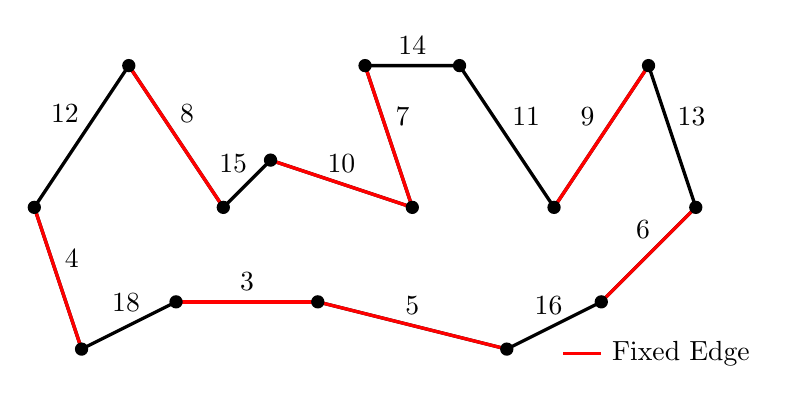
\begin{tikzpicture}[thick,scale=.6]
            \coordinate (A) at (0, 0);\coordinate (B) at (2, 3);\coordinate (C) at (4, 0);\coordinate (D) at (1, -3);\coordinate (E) at (3, -2);\coordinate (F) at (5, 1);\coordinate (G) at (6, -2);\coordinate (H) at (8, 0);\coordinate (I) at (7, 3);\coordinate (J) at (9, 3);\coordinate (K) at (11, 0);\coordinate (L) at (10, -3);\coordinate (M) at (12, -2);\coordinate (N) at (14, 0);\coordinate (O) at (13, 3);

            \draw[-,very thick] (A) -- node[above,yshift=1,xshift=-6] {12} (B) -- node[above,yshift=1,xshift=4] {8} (C) --node[above,xshift=-5] {15} (F) -- node[above] {10} (H) -- node[above,xshift=5] {7} (I) -- node[above] {14} (J) -- node[above,xshift=7] {11} (K) -- node[above,xshift=-5] {9} (O) -- node[above,xshift=7] {13} (N) -- node[above,yshift=2,xshift=-2] {6} (M) -- node[above,xshift=-2] {16} (L) -- node[above] {5} (G) -- node[above] {3} (E) -- node[above,yshift=1,xshift=-1] {18} (D) -- node[above,xshift=5] {4} (A);
            \draw[-,very thick, Red] (G) -- (E);
            \draw[-,very thick, Red] (D) -- (A);
            \draw[-,very thick, Red] (L) -- (G);
            \draw[-,very thick, Red] (N) -- (M);
            \draw[-,very thick, Red] (B) -- (C);
            \draw[-,very thick, Red] (H) -- (I);
            \draw[-,very thick, Red] (K) -- (O);
            \draw[-,very thick, Red] (F) -- (H);

            \foreach \point in {A, B, C, D, E, F, G, H, I, J, K, L, M, N, O} {
                \fill (\point) circle (4pt);
            }

            \draw [-,very thick,Red] (11.2,-3.1) --  (12,-3.1) node[anchor=west, black] {Fixed Edge};
        \end{tikzpicture}
	    \caption{Example of a smallest edges fix of 8 edges} \label{fig:exampleSmallFix}
    \end{figure}
    \item \textbf{Sequence Fix}\\
    Fixing along a sequence means that edges are locked starting from a node, following the path of the known solution until the desired number of nodes have been locked.
    On the upside this technique allows to optimize contigous sections of the solution, resulting in a solution that is composed of a sequence of optimal paths.
    The disadvantage of this method is that it permits only localized moves, thereby neglecting optimizations that consider the problem from a broader perspective.
    \begin{figure}[H]
        \centering
        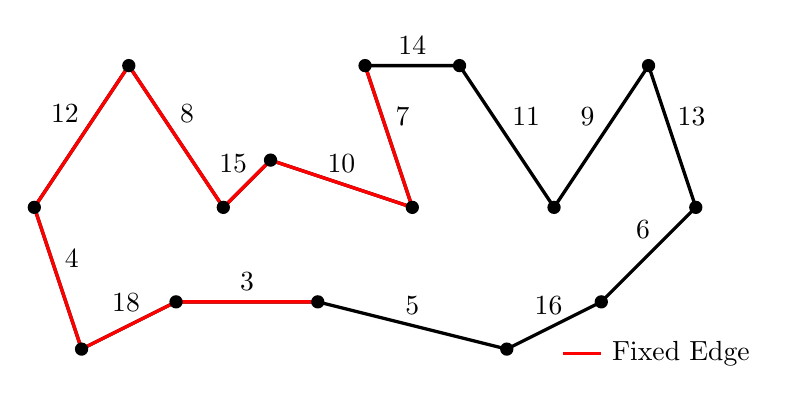
\begin{tikzpicture}[thick,scale=.6]
            \coordinate (A) at (0, 0);\coordinate (B) at (2, 3);\coordinate (C) at (4, 0);\coordinate (D) at (1, -3);\coordinate (E) at (3, -2);\coordinate (F) at (5, 1);\coordinate (G) at (6, -2);\coordinate (H) at (8, 0);\coordinate (I) at (7, 3);\coordinate (J) at (9, 3);\coordinate (K) at (11, 0);\coordinate (L) at (10, -3);\coordinate (M) at (12, -2);\coordinate (N) at (14, 0);\coordinate (O) at (13, 3);

            \draw[-,very thick] (A) -- node[above,yshift=1,xshift=-6] {12} (B) -- node[above,yshift=1,xshift=4] {8} (C) --node[above,xshift=-5] {15} (F) -- node[above] {10} (H) -- node[above,xshift=5] {7} (I) -- node[above] {14} (J) -- node[above,xshift=7] {11} (K) -- node[above,xshift=-5] {9} (O) -- node[above,xshift=7] {13} (N) -- node[above,yshift=2,xshift=-2] {6} (M) -- node[above,xshift=-2] {16} (L) -- node[above] {5} (G) -- node[above] {3} (E) -- node[above,yshift=1,xshift=-1] {18} (D) -- node[above,xshift=5] {4} (A);
            \draw[-,very thick, Red] (G) -- (E) -- (D) -- (A) -- (B) -- (C) -- (F) -- (H) -- (I);

            \foreach \point in {A, B, C, D, E, F, G, H, I, J, K, L, M, N, O} {
                \fill (\point) circle (4pt);
            }

            \draw [-,very thick,Red] (11.2,-3.1) --  (12,-3.1) node[anchor=west, black] {Fixed Edge};
        \end{tikzpicture}
	    \caption{Example of a sequence fix of 8 edges} \label{fig:exampleSeqFix}
    \end{figure}
\end{itemize}
Since every one of these techniques have different advantages and disadvantages, we chose to mix them all together by selecting at random which method to use to fix edges at every iteration.
Even by using all of these procedure together there is the risk of getting stuck in a local minima.
To roughly detect the local minima one can simply check how many iterations from the last improving iteration have been performed.
There surely are many ways to escape a local minimum point, one of the simplest is to just reduce the amount of fixed edges once the solution stops improving.
After a threshold value of not-improving iterations has been reached, decrease the number of fixed edges.
In this implementation, the starting number of fixed edges is 10\% the number of nodes and it is decreased with steps of equal size.
\begin{figure}[htbp]
	\begin{algorithm}[H]
        \TitleOfAlgo{\textbf{Hard Fixing}}
		\SetKwInOut{Input}{input}
        \SetKwInOut{Output}{Output}
		\Input{
			Starting solution $s$ \newline
            Time limit $tlim$ \newline
            Number of edges to fix $n$ \newline
            Stagnant iterations threshold $iterThresh$
		}
        \Output{Improved solution $s$}
		\vspace{2mm}
        $p \gets$ CPLEX Initialization \\
        $i \gets 0$ \\ 
        \While{$time < tlim$}{
            fix $n$  edges in $p$ according to one of the 3 methods chosen at random\\
            run Branch and Cut on $p$ \\
            $x^* \gets$ optimal solution of $p$ (w.r.t. the fixed edges) \\
            $s' \gets$ convert $x^*$ to successors solution \\
            \eIf{$cost(s') < cost(s)$}{
                $s \gets s'$\\
                $i \gets 0$
            }{
                $i++$\\
                \lIf{$i = iterThresh$}{
                    \textbf{decrease} $n$
                }
            }
            \uIf{$n$ = 0}{
                \textbf{break}
                \tcp{Optimal solution found}
            }
            un-fix all previously fixed edges in $p$
        }
        \textbf{return} $s$
	\end{algorithm}
	\caption{Pseudocode of the Hard Fixing algorithm} \label{fig:hardfix}
\end{figure}

\subsection{Performance}

\begin{table}[htbp]
	\centering
	\begin{tabular}{|c|c|}
        \hline \textbf{Instance size} & \textbf{Time limit} \\
		\hline 0-80 & 1 \\
		\hline 100-200 & 3 \\
        \hline 220-320 & 8 \\
        \hline 400-500 & 20 \\
        \hline 500-800 & 60 \\
        \hline 1000-1440 & 180 \\
        \hline 1570-2400 & 400 \\
        \hline
	\end{tabular}
    \vspace{2mm}    
	\caption{Time limit for matheuristics} \label{tab:mathheurTlim}
\end{table}

Even though matheuristics are written on top of the exact method Branch and Cut, their output is not guaranteed to be optimal since, from a high level viewpoint, their behavior is more comparable to a metaheuristic.
Therefore it makes sense for algorithms like Hard Fixing to be analyzed on the quality of the output solution rather than their efficiency like with the exact methods.

\figurename{ \ref{fig:hardfixCost}} shows the difference between the cost of the solution used as input, the output solution as well as the optimal solution, in order to derive meaningful conclusion on the performance of the algorithm.
\begin{figure}[htbp]
	\centering
    \begin{tikzpicture}
        \begin{axis}[
            xlabel={Cost Ratio},     % AXIS NAME
            %ylabel={Iterations/s Ratio},   % AXIS NAME
            xmin=1, xmax=1.1,       % AXIS LIMITS
            ymin=0, ymax=67,        % AXIS LIMITS
            xtick={},
            ytick=\empty,
            legend style={at={(0.98,0.02)},anchor=south east,legend columns=1}, %MOVE LEGEND HERE
			legend cell align={left},
            %ymajorgrids=true,
            xmajorgrids=true,
            grid style=dashed,
        ]
        
        \addplot[Blue,mark=square,mark size=1.5] table[x=startcost,y=idx, col sep=semicolon] {csv/hardfix_cost.csv}; 
        \addplot[Red,mark=o,mark size=1.5] table[x=finalcost,y=idx, col sep=semicolon] {csv/hardfix_cost.csv};
        \addplot[Green,mark=triangle,mark size=1.5] table[x=optimalcost,y=idx, col sep=semicolon] {csv/hardfix_cost.csv}; 
        \addlegendentry{Starting Cost} 
        \addlegendentry{Final Cost}
        \addlegendentry{Optimal Cost}
            
        \end{axis}
    \end{tikzpicture}
	\caption{Performance profile graph of Hard Fixing\label{fig:hardfixCost}}
\end{figure}
Like with the other algorithms using CPLEX shown before, the time limit set to find the initial solution was set to 1\% of the full time limit.
The initial solution was obtained using Nearest Neighbor and 2-Opt.

% \begin{table}[htbp]
% 	\centering
% 	\begin{tabular}{c|c|c|}
%         & \textbf{Optimization Amount} & \textbf{Distance from Optimal} \\
% 		\hline \textbf{mean} & 3.34\% & 0.96\% \\
% 		\hline \textbf{std dev} & 1.70\% & 1.08\% \\
%         \hline \textbf{Q(25\%)} & 2.23\% & 0.14\% \\
%         \hline \textbf{Q(50\%)} & 3.39\% & 0.47\% \\
%         \hline \textbf{Q(75\%)} & 4.25\% & 1.42\% \\
% 	\end{tabular}
%     \vspace{2mm}
% 	\caption{Statistics on results from Hard Fixing} \label{tab:hardfixStats}
% \end{table}

\section{Local Branching}

Local Branching is a matheuristic technique that basically performes a series of “k-Opt” move to improve the solution.
Like Hard Fixing, it begins with a feasible initial solution, which can be generated using various heuristics or metaheuristics which serves as a starting point for the local branching process.
In Local Branching, a neighborhood of the current solution is defined by introducing additional constraints, that we will refer to as \textbf{local branching constraints}.
These constraints limit the search to a subset of solutions that are close to the current solution in terms of some predefined criteria, such as the number of differing edges in the TSP tour.

By restricting the search to this localized region, the optimization process can focus on improving the solution within a manageable computational effort.
The optimization within this local neighborhood is performed using mathematical programming techniques, in this case, the Branch and Cut algorithm implemented with CPLEX is used.
The solver explores this restricted solution space to find an improved solution.
If an improved solution is found, it becomes the new incumbent solution, and a new neighborhood is defined around it.
This iterative process of defining local neighborhoods and optimizing within them continues until a stopping criterion is met, which in our case is a time limit.

\begin{figure}[htbp]
    \centering
    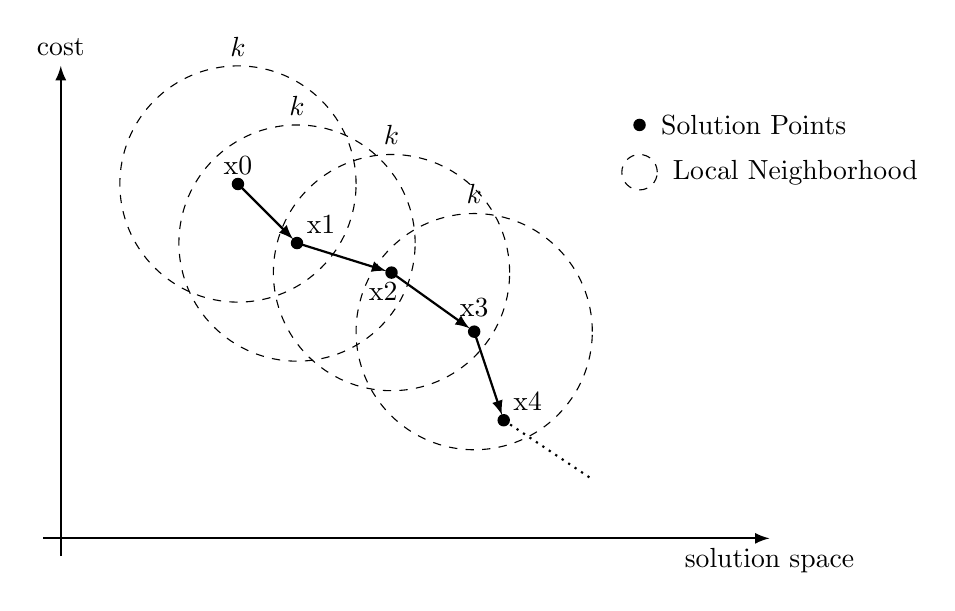
\begin{tikzpicture}[scale=.75]

        \draw[-latex,thick] (-6,-2.3) -- (-6,6) node[above]{cost};
        \draw[-latex,thick] (-6.3,-2) -- (6,-2) node[below]{solution space};

        % Define coordinates for initial, intermediate, and final solutions
        \coordinate (init) at (-3, 4);
        \coordinate (int1) at (-2, 3);
        \coordinate (int2) at (-0.4, 2.5);
        \coordinate (int3) at (1, 1.5);
        \coordinate (final) at (1.5, 0);
        \coordinate (beyond) at (3,-1);
        
        % Draw the initial, intermediate, and final solutions as points
        \fill (init) circle (3pt) node[above] {x0};
        \fill (int1) circle (3pt) node[above right] {x1};
        \fill (int2) circle (3pt) node[below, xshift=-3] {x2};
        \fill (int3) circle (3pt) node[above, yshift=2] {x3};
        \fill (final) circle (3pt) node[above right] {x4};
        
        % Draw arrows to show the progression
        \draw[-latex,thick,shorten <=2pt,shorten >=2pt] (init) -- (int1);
        \draw[-latex,thick,shorten <=2pt,shorten >=2pt] (int1) -- (int2);
        \draw[-latex,thick,shorten <=2pt,shorten >=2pt] (int2) -- (int3);
        \draw[-latex,thick,shorten <=2pt,shorten >=2pt] (int3) -- (final);
        \draw[thick,dotted] (final) -- (beyond);
        
        % Draw a few example neighborhoods
        \draw[dashed] (init) circle (2) + (0,2) node[above]{$k$};
        \draw[dashed] (int1) circle (2) + (0,2) node[above]{$k$};
        \draw[dashed] (int2) circle (2) + (0,2) node[above]{$k$};
        \draw[dashed] (int3) circle (2) + (0,2) node[above]{$k$};
        
        % Add a legend
        \fill (3.8, 5) circle (3pt);
        \node[right] at (4, 5) {Solution Points};
        \draw[dashed] (3.8, 4.2) circle (0.3);
        \node[right] at (4.2, 4.2) {Local Neighborhood};
        
    \end{tikzpicture}
	\caption{Example of Local Branching optimizing iterations } \label{fig:locBrancSolDescent}
\end{figure}    

The implementation of this matheuristic is not much different from the implementation of Hard Fixing.
Of course we used the initial solution to initialize the CPLEX problem and the Branch and Cut algorithm as well.
The difference with Hard Fixing is in the way the CPLEX problem is modified: instead of changing the lower bound of variables we add new constraint.
Given $n$ as the number of nodes, $S = \{(a,b),(b,c),(c,d),...\}$ as the starting solution, $|S| = n$, and $k$ as the neighborhood size, the \textbf{locality constraint} is defined as follows.
\[
    \sum_{e \in S} x_e >= n-k
\]
Of course, as it was the case with all 2-Opt, there is the risk in becoming stuck into a local minima solution for a given value of $k$.
When that happens, metaheuristics like Variable Neighborhood Search and Tabu Search used the techniques of performing some kind of non-improving moves in order to escape the local minimum point.
In Local Branching it's not necessary to use such a technique since it's possible to increase $k$ without requiring any additional efforts, allowing to escape the local minima at the cost solving a harder problem with Branch and Cut.
After the algorithm escapes the critical point it's possible to reduce again the value of $k$, to return to the original problem complexity.
In this implementation $k$ starts out with the value of 10 and it is increased, when necessary, by 5.

\begin{figure}[htbp]
	\begin{algorithm}[H]
        \TitleOfAlgo{\textbf{Local Branching}}
		\SetKwInOut{Input}{input}
        \SetKwInOut{Output}{Output}
		\Input{
			Starting solution $s$ \newline
            Time limit $tlim$ \newline
            Neighborhood size $k$
		}
        \Output{Improved solution $s$}
		\vspace{2mm}
        $p \gets$ CPLEX Initialization \\
        $i \gets 0$ \\ 
        \While{$time < tlim$}{
            add locality constraint to $p$\\
            run Branch and Cut on $p$ \\
            $x^* \gets$ optimal solution of $p$ (w.r.t. the restricted solution space) \\
            $s' \gets$ convert $x^*$ to successors solution \\
            \eIf{$cost(s') < cost(s)$}{
                $s \gets s'$
            }{
                \textbf{increase} $k$\\
            }
            \uIf{$k$ = number of nodes}{
                \textbf{break}
                \tcp{Optimal solution found}
            }
            remove locality constraint from $p$
        }
        \textbf{return} $s$
	\end{algorithm}
	\caption{Pseudocode of the Local Branching algorithm} \label{fig:localBranching}
\end{figure}

\subsection{Performance}

We performed the testing using the same settings, the same time limits as well as the same instances as with Hard Fixing data collection.

\begin{figure}[htbp]
	\centering
	\begin{tikzpicture}
        \begin{axis}[
            xlabel={Cost Ratio},     % AXIS NAME
            %ylabel={Iterations/s Ratio},   % AXIS NAME
            xmin=1, xmax=1.1,       % AXIS LIMITS
            ymin=0, ymax=67,        % AXIS LIMITS
            xtick={},
            ytick=\empty,
            legend style={at={(0.98,0.02)},anchor=south east,legend columns=1}, %MOVE LEGEND HERE
			legend cell align={left},
            %ymajorgrids=true,
            xmajorgrids=true,
            grid style=dashed,
        ]
        
        \addplot[Blue,mark=square,mark size=1.5] table[x=startcost,y=idx, col sep=semicolon] {csv/local-branching_cost.csv}; 
        \addplot[Red,mark=o,mark size=1.5] table[x=finalcost,y=idx, col sep=semicolon] {csv/local-branching_cost.csv};
        \addplot[Green,mark=triangle,mark size=1.5] table[x=optimalcost,y=idx, col sep=semicolon] {csv/local-branching_cost.csv}; 
        \addlegendentry{Starting Cost} 
        \addlegendentry{Final Cost}
        \addlegendentry{Optimal Cost}
            
        \end{axis}
    \end{tikzpicture}
	\caption{Performance profile graph of Local Branching\label{fig:localBranchingCost}}
\end{figure}

% \begin{table}[htbp]
% 	\centering
% 	\begin{tabular}{c|c|c|}
%         & \textbf{Optimization Amount} & \textbf{Distance from Optimal} \\
% 		\hline \textbf{mean} & 2.70\% & 1.55\% \\
% 		\hline \textbf{std dev} & 1.81\% & 1.80\% \\
%         \hline \textbf{Q(25\%)} & 1.24\% & 0.00\% \\
%         \hline \textbf{Q(50\%)} & 2.56\% & 0.76\% \\
%         \hline \textbf{Q(75\%)} & 3.84\% & 2.79\% \\
% 	\end{tabular}
%     \vspace{2mm}
% 	\caption{Statistics on results from Local Branching} \label{tab:localBranchingStats}
% \end{table}

\section{Comparison}
To conclude this chapter, \figurename{ \ref{fig:hardFixLocBranchCMP}} provides graphical means to compare the quality of the solutions of Hard Fixing and Local Branching.
It is clear that Hard Fixing holds is a superior algorithm given the same time limit, but this is just another case of an algorithm being faster than the other one.
The significantly higher number of iterations performed by Hard Fixing questions the autenticity of the results and poses another question: would local branching perform better or worse if enough time is given to match Hard Fixing speed?
To answer this question we would need to gather and studied a significant amount of data and, while this is still a valuable experiment, it is beyond the scope of this project.
Considering the limited resources available, we concluded that this implementation of Hard Fixing is generally superior to the Local Branching method and that changing the bounds of some variables in a CPLEX problem is more effective than to introduce a new constraint.
However, it remains unclear whether Hard Fixing is both more effective and faster, or if its faster execution simply allows it to achieve better results within the same timeframe.

\begin{figure}[htbp]
	\centering
	\begin{tikzpicture}
        \begin{axis}[
            xlabel={Cost Ratio},     % AXIS NAME
            %ylabel={Iterations/s Ratio},   % AXIS NAME
            xmin=1, xmax=1.06,       % AXIS LIMITS
            ymin=0, ymax=67,        % AXIS LIMITS
            xtick={},
            ytick=\empty,
            legend style={at={(0.98,0.02)},anchor=south east,legend columns=1}, %MOVE LEGEND HERE
			legend cell align={left},
            %ymajorgrids=true,
            xmajorgrids=true,
            grid style=dashed,
        ]
        
        \addplot[Blue,mark=square,mark size=1.5] table[x=hardfix_cost, y=idx, col sep=semicolon] {csv/cmp_hardfix_local-branching.csv}; 
        \addplot[Red,mark=o,mark size=1.5] table[x=localbranch_cost, y=idx, col sep=semicolon] {csv/cmp_hardfix_local-branching.csv};
        \addlegendentry{Hard Fixing} 
        \addlegendentry{Local Branching}
            
        \end{axis}
    \end{tikzpicture}
	\caption{Comparison between Hard Fixing and Local Branching solution quality \label{fig:hardFixLocBranchCMP}}
\end{figure}

\begin{figure}[htbp]
	\centering
	\begin{tikzpicture}
        \begin{axis}[
            ylabel={Iterations/s Ratio},     % AXIS NAME
            xlabel={Sorted instances},   % AXIS NAME
            xmin=0, xmax=67,       % AXIS LIMITS
            ymin=1, ymax=57,        % AXIS LIMITS
            ytick={1,10,20,30,40,50},
            xtick=\empty,
            legend style={at={(0.02,0.98)},anchor=north west,,legend columns=1}, %MOVE LEGEND HERE
			legend cell align={left},
            ymajorgrids=true,
            %xmajorgrids=true,
            grid style=dashed,
        ]
        
        \addplot[Blue,mark=square,mark size=1.5] table[y=hardfix_iter, x=idx, col sep=semicolon] {csv/cmp_hardfix_local-branching.csv}; 
        \addplot[Red,mark=o,mark size=1.5] table[y=localbranch_iter, x=idx, col sep=semicolon] {csv/cmp_hardfix_local-branching.csv};
        \addlegendentry{Hard Fixing} 
        \addlegendentry{Local Branching}
            
        \end{axis}
    \end{tikzpicture}
	\caption{Comparison between Hard Fixing and Local Branching iterations/s \label{fig:hardFixLocBranchIterCMP}}
\end{figure}

Finally we can compare metaheuristics and matheuristics, specifically comparing the performance between VNS and Hard Fixing which are the best algorithms in each section and we can see that VNS yields overall better performance when compared to Hard Fixing.

\begin{figure}[htbp]
	\centering
	\begin{tikzpicture}
        \begin{axis}[
            xlabel={Cost Ratio},     % AXIS NAME
            %ylabel={Iterations/s Ratio},   % AXIS NAME
            xmin=1, xmax=1.06,       % AXIS LIMITS
            ymin=0, ymax=66,        % AXIS LIMITS
            xtick={},
            ytick=\empty,
            legend style={at={(0.98,0.02)},anchor=south east,legend columns=1}, %MOVE LEGEND HERE
			legend cell align={left},
            %ymajorgrids=true,
            xmajorgrids=true,
            grid style=dashed,
        ]
        
        \addplot[Blue,mark=square,mark size=1.5] table[x=vns, y=idx, col sep=semicolon] {csv/vnshardfix.csv}; 
        \addplot[Red,mark=o,mark size=1.5] table[x=hardfix, y=idx, col sep=semicolon] {csv/vnshardfix.csv};
        \addplot[Green,mark=triangle,mark size=1.5] table[x=opt, y=idx, col sep=semicolon] {csv/vnshardfix.csv};
        \addlegendentry{VNS}
        \addlegendentry{Hard Fixing}
        \addlegendentry{Optimal}
            
        \end{axis}
    \end{tikzpicture}
	\caption{Comparison between Hard Fixing and VNS} \label{fig:vnshardfix}
\end{figure}





\begin{thebibliography}{9}
	\bibitem{tsplib}
	\url{http://comopt.ifi.uni-heidelberg.de/software/TSPLIB95/}

	\bibitem{avxWikipedia}
	\url{https://en.wikipedia.org/wiki/Advanced_Vector_Extensions}

\end{thebibliography}

\end{document}

